% ==============================================================
% File     : main.tex
% Date     : 03 Apr. 2022
% Revision : 30 July 2022
% Creator  : Marco Peressutti
% ==============================================================

\documentclass[a4paper, 10pt, oneside]{book}
\usepackage[utf8]{inputenc}


\usepackage[right=30.2mm, left=28.4mm,marginparwidth=75pt,  top=20mm]{geometry}
%\usepackage[a4paper, marginparwidth=75pt, total={10cm, 10cm}]{geometry}
\usepackage[english]{babel}
\usepackage{lmodern}
\usepackage[T1]{fontenc}
\usepackage{graphicx}
\usepackage{microtype}
\usepackage{amsmath, amssymb, mathtools, amsthm}
\usepackage{dirtytalk}
\usepackage{csquotes}
\usepackage[acronym, nonumberlist, seeautonumberlist]{glossaries}
\usepackage[bibstyle=numeric, backend=biber, sorting=nty]{biblatex}
\usepackage{subcaption}
\usepackage{marginnote}
\usepackage{todonotes}
\usepackage{hyperref}
\usepackage[makeroom]{cancel}
\usepackage{setspace}
\usepackage{nicematrix}
\usepackage{tabularx}
\usepackage{booktabs}
\usepackage{empheq}
\usepackage{enumitem}
\usepackage{xfrac}
\usepackage{makecell}
\usepackage{pifont}
\usepackage{minitoc}

\usepackage{xpatch}

\usepackage{xcolor}
\usepackage{listings} % usepackages
% ==============================================================
% File     : lib/acronyms.tex
% Date     : 03 Apr. 2022
% Revision : 03 Apr. 2022
% Creator  : Marco Peressutti
% ==============================================================
 % acromyms
\defbibheading{bibempty}{}

\newcommand{\M}[1]{\begin{bmatrix}#1\end{bmatrix}}
\newcommand{\und}[1]{\underline{#1}}
\newcommand{\B}[1]{\begin{Bmatrix}#1\end{Bmatrix}}
\newcommand{\pd}[2]{\cfrac{\partial#1}{\partial#2}}
\newcommand{\td}[2]{\cfrac{d#1}{d#2}}
\newcommand{\tdd}[2]{\cfrac{d^2#1}{d#2^2}}
\newcommand{\pdd}[2]{\cfrac{\partial^2#1}{\partial#2^2}}
\renewcommand{\theta}{\vartheta}
\newcommand{\omissis}{[\textellipsis\unkern]}
\newcommand{\pexp}[2]{\prescript{#1}{}{#2}{}{}}
\newcommand{\ret}[1]{{#1}^{\leftarrow}}
\renewcommand{\epsilon}{\varepsilon}
\newcommand{\smalltodo}[2][]{\todo[caption={#2}, #1, backgroundcolor=white!20!white, bordercolor=white]{\begin{spacing}{0.5}\texttt{#2}\end{spacing}}}
\newcommand{\side}[1]{\smalltodo[size=\footnotesize]{#1}\textbf{#1}}
\newcommand{\pside}[1]{\smalltodo[size=\footnotesize]{#1}}
\DeclarePairedDelimiter\abs{\lvert}{\rvert}
\DeclarePairedDelimiter{\norma}{\lVert}{\rVert}
\newcommand{\degr}[1]{^{\circ\!#1}}
\DeclareMathOperator*{\minimize}{minimize}
\DeclareMathOperator*{\argmin}{argmin}
\DeclareMathOperator*{\argmax}{argmax}
\newtheorem{theorem}{Theorem}

\makeatletter
\newcommand\incircbin
{%
  \mathpalette\@incircbin
}
\newcommand\@incircbin[2]
{%
  \mathbin%
  {%
    \ooalign{\hidewidth$#1#2$\hidewidth\crcr$#1\bigcirc$}%
  }%
}
\newcommand{\ooplus}{\incircbin{+}}
\newcommand{\oominus}{\incircbin{-}}
\newcommand{\oocirca}{\incircbin{\sim}}
\makeatother

\renewcommand{\arraystretch}{1.3}
\setitemize{noitemsep,topsep=10pt,parsep=0pt,partopsep=0pt}
\newcommand{\cmark}{\ding{51}}
\newcommand{\xmark}{\ding{55}}
\newcommand{\cge}{\succeq}
\newcommand{\cle}{\precceq}
\newcommand{\cless}{\precc}
\newcommand{\cmore}{\succ}

\setcounter{minitocdepth}{3}

\definecolor{codegreen}{rgb}{0,0.6,0}
\definecolor{codegray}{rgb}{0.5,0.5,0.5}
\definecolor{codepurple}{rgb}{0.58,0,0.82}
\definecolor{backcolour}{rgb}{0.95,0.95,0.92}

\lstdefinestyle{mystyle}{
    backgroundcolor=\color{backcolour},   
    commentstyle=\color{codegreen},
    keywordstyle=\color{magenta},
    numberstyle=\tiny\color{codegray},
    stringstyle=\color{codepurple},
    basicstyle=\ttfamily\footnotesize,
    breakatwhitespace=false,         
    breaklines=true,                 
    captionpos=b,                    
    keepspaces=true,                 
    numbers=left,                    
    numbersep=5pt,                  
    showspaces=false,                
    showstringspaces=false,
    showtabs=false,                  
    tabsize=2
}

\lstset{style=mystyle} % newcommands

% title page
\title{Distributed Artificial Intelligence\\and\\ Intelligent Agents}
\author{Marco Peressutti}
\date{\today}

% chapters
\includeonly{
    chapters/00-Introduction,
    chapters/01-Negotiation,
    chapters/02-Communication,
    chapters/03-Coordination,
    chapters/04-MASArchitecture,
    chapters/05-AOSE,
    chapters/06-Theory,
    chapters/07-Architecture,
    chapters/08-MLandRL,
    chapters/09-Mobility
}


% bibliography resources
\addbibresource{bib/bibliography.bib}
% path to images
\graphicspath{{images/}}
% load acronyms
\makeglossaries

\begin{document}
    \selectlanguage{english}
 
    \maketitle

    \frontmatter
    \setcounter{page}{1}
    \cleardoublepage

    \fancypagestyle{plain}{}

    \renewcommand{\chaptermark}[1]{ \markboth{#1}{}} 
    \dominitoc[n]
    \tableofcontents
      \markboth{\contentsname}{}      
    \cleardoublepage

    %% mainmatter
    \mainmatter



    %\tableofcontents
%
    %\clearpage
    %\setcounter{page}{1}
    %% mainmatter

    \chapter{Introduction}
\minitoc

\section{Definition of an Agent}
\begin{itemize}
\item an agent has \side{independent behaviour}: when there is no possibility for direct supervision
\item agents \side{collaborate} and \side{communicate} with each other
\item angets have \side{proactive behaviour}: they have the reasoning possibility to proactively propose some solutions
\item \side{privacy ensurance}: privacy should be ensured via \side{personalization}. A person's interest should not be disclouse to some external entity other than the agent itself.
\end{itemize}

\subsection{Formal definitions}
\begin{enumerate}
\item American Heritage Dictionary:

\say{One that acts or has the power or authority to \textbf{act} ... or \textbf{represent} another}

Agents are not independent entitities that operate by their own view but they always represent some interest of those who create them.
\item Negroponte

\say{Digital sister in law}

Agents should have specialized expertise and knowledge of preferences of those who create them
\item Russel and Norvig

\say{An agent is anything that can be viewed as perceiving its environment through sensors and acting upon that environment through effectors.}
\item Pattie Maes

\say{Autonomous Agents are computational systems that \textbf{inhabit} some complex dynamic environment, \textbf{sense} and \textbf{act} autonomously in this environment, and by doing so \textbf{realize} a set of goals or tasks for which they are designed}

Agents leave in an environment.
\item IBM

\say{Intelligent agents are software entities that carry out some set of \textbf{operations on behalf of} a user or another program with some degree of \textbf{independence} or \textbf{autonomy}, and in doing so, employ some \textbf{knowledge} or \textbf{representations} of the user’s \textbf{goals} or \textbf{desires}}
\item Coen

\say{Software agents are programs that engage in dialog [and] \textbf{negotiate} and \textbf{coordinate} transfer of information}

Agents must have the possibility to communicate and consequently coordinate and negotiate with one another.
\end{enumerate}

\subsection{Logicale behind autonomous systems}
\begin{itemize}
\item More and more everyday tasks are computer based
\item The world is in a midst of an information revolution
\item increasingly more users are untrained
\item \side{Lack of programming paradigm} for decentralized program/system construction in dynamic environment.

Existing paradigms were constructed for closed world (i.e. completely specified environment).\\
However in AI the environment is not specified completely (hence there is the need for dynamic exploration of the environment).
\end{itemize}

The solution to this lack of paradigm is to \side{emulate human behaviour}, therefore agents must be able to:
\begin{itemize}
\item perceive the environment
\item affect the environement or act in the environment
\item have a \side{model of behaviour}
\item have intentions/motivations to be fulfilled by implementing corresponding goals.\\
In fact, goals are not enough, the sytem needs to generate new goals from its intentions and beliefs.
\item communication
\end{itemize}

\subsection{Agent definition and properties}
Wooldridge, Jennings (\side{weak notion}):\\
\say{Agent is a hardware or (more usually) software-based computer system that enjoys the following properties:}
\begin{itemize}
\item \side{autonomy}.\\
Agents operate without the direct intervention of humans or others, and have some kind of control over their actions and internal state.

Hence in order for an agent to be autonomous it must:
\begin{itemize}
\item Act indipendently
\item Have control over its internal state.

Contrary to objects, agents need to encapsulate behaviour other than their state in the environment.\\
They, in fact, differs from objects since they are required to have a:
\begin{enumerate}
\item \side{degree of autonomy}: agents embody a stronger notion of autonomy than objects, in particular, agents decide for themselves whether or not to perform an action.
\item \side{degree of smartness}: capable of flexible (reactive, pro-active, social) behaviour; standard object models do not have such behaviour
\item \side{degree of activeness}: a multi-agent system is inherently multi-threaded in that each agent is assumed to have at least one thread of active control.
\end{enumerate}
\end{itemize}
\item \side{pro-activeness}.\\
Agents do not simply act in response to their environment, they are able to exhibit goal-directed behavior by taking the initiative.\\
In short, agent smust be able to create goals on their own intiative.
\item \side{reactivity}.\\
Agents perceive their environment and respond in a timely fashion to changes that occur in it.\\
In short, communication with the environment.
\item \side{social ability}.\\
Agents interact with other agents (and possibly humans) via some kind of agent-communication language.\\
In short, communication with other agents
\end{itemize}


Wooldridge, Jennings (\side{strong notion}):\\
\begin{itemize}
\item \side{Mentalistic notions}, such as beliefs and intentions are often referred to as properties of strong agents
\item \side{Veracity}, agents will not knowingly communicate false information
\item \side{Benevolence}: agents do not have conflicting goals and always try to do what is asked of it
\item \side{Rationality}: an agent will act in order to achieve its golas and will not act in such a way as to prevent its goals being achieved
\item \side{Mobility}: the ability of an agent to move around a network
\end{itemize}

In addition to these basic properties several other alternatives have been proposed over the years:
\begin{enumerate}
\item Isaac Asimov's laws of robotics:
\begin{enumerate}[label={Law}]
\item One\\
A ropbot may not injure a human being or, through inaction, allow a human being to come to harm
\item Two\\
A robot must obey orders given to it by human beings except where such orders would conflict with the First Law
\item Three\\
A robot must protect its own existence, as long as such protection does not conflict with the First or Second Law
\item Zeroth\\
A robot may not harm humanity, or, by inaction, allow humanity to come to harm
\end{enumerate}
\item A robot must establish its identity as a robot in all cases
\item A robot must know it is a robot
\item A robot must reproduce. As long as such reproduction does not contradict with Laws 1,2 and 3
\item All robots endowed with comparable human reason and conscience should act towards one another in a spirit of brotherhood
\end{enumerate}

\vfill
Summary:
\begin{itemize}
\item Agents acts on behalf of other entities
\item Agents must have weak agent characteristics
\item Agents may have strong agent characteristics
\end{itemize}

\section{Individual and Group Perspective}
There are two fundamental agents dimensions:
\begin{itemize}
\item \side{Individual agents perspective}. That deals with how to  build agents that are capable of independent autonomous actions in order to successfully carry out the tasks that we delegate to them (\side{Micro aspects}).
\item \side{Group agents perspective}. That deals with how to build agents that are capable of interacting (cooperating, coordinating, negotating) with other agents in order to successfully carry out the tasks we delegate to them (\side{Macro aspects}).
\end{itemize}

\section{Distributed AI and MAS}
\begin{itemize}
\item Distributed AI is a topic/subject rather than the creation of a brain that is distributed.
\item It became part of AI when it was possible to execute on more than one CPU.
\item For this reason, it is often considered as the intersection of \side{Distributed Computing} and \side{Aritificial Intelligence}.
\missingfigure{}
\item Distributed AI includes two different subfield: \side{Distributed Problem Solving (DPS)} and \side{Multi-Agent Systems (MAS)}.
\item DAI deals with several aspects and dimensions such as:
\begin{itemize}
\item Agent granularity
\item Heterogeneity of agents
\item Communication possibilities
\item Methods of distributing control among agents
\end{itemize}
\end{itemize}


\subsection{Distributed Problem Solving (DPS)}
DPS considers how the task of solving a particular problem can be divided among a number of modules that cooperate in dividing and sharing knowledge about the problem and its evolving solution(s):
\begin{itemize}
\item In pure DPS systems, all interaction strategies are incorporate as an integral part of the system
\item DPS has focused on achieving goals under varying environmental conditions, having agents with established properties
\end{itemize}

In other terms in DPS:
\begin{enumerate}
\item a problem is divided into modules 
\item each module is allocated to a different agent
\item the agents will solve the problem by means of communicating the solution to their allocated module
\end{enumerate}

\subsection{Multi-Agent Systems (MAS)}
\begin{itemize}
\item MAS are designed in a decentralized way with great part of independency and autonomy
\item Agents with individual preferences will interact in particular environments such that each will consent to act in a way that leads to desired global goal
\item MAS asks how, for a particular environment, can certain collective goal be realized if the properties of agents can vary uncontrollably:
\begin{itemize}
\item loosely-coupled networks of problem solvers (agents) that work together to solve problems that are beyond their capabilities
\item no necessary guarantees about other agent
\end{itemize}
\item MAS contain a number of agents which interact with one another through communication. The agetns are able to act in an environment; where each agent will act upon or influence different parts of the environment. If two field of influence overlap, the conflict is (hopefully) resolved via negotiation and communication
\missingfigure{}
\item An important concept in MAS is that there is no central control (because the control is distributed to the various agents) and knowledge or information sources may also be distributed
\end{itemize}

In other terms, contrary to DPS, MAS do not deal with task to be solved but rather rules to be followed, and these rules are for example, their beliefs, desire and intentions or protocols for negotiation and communication.

The motives behind the use of MAS are:
\begin{itemize}
\item To solve problems that are too large for a centralized agent
\item To allow interconnection and interoperation of multiple legacy systems
\item To provide a solution to inherently distributed problems
\item To provide solutions which draw from distributed information sources
\item To provide solutions where expertise is distributed
\item To offer conceptual clarity and simplicity of design
\end{itemize}

The are two subclasses of MAS:
\begin{itemize}
\item \side{Cooperative}.

Agents are designed by interdependent designers.\\
Agents act for increased good of the system.\\
Agents are concerned with increasing the performance of the system.\\

Hence if we imagine that the goodness of the system is represented by a gloabal function. Agents in a cooperative MAS will try to maximize such function.
\item \side{Self-interested}

Agents designed by independent designers.\\
Agents have their own agenda and motivation.\\
Agents are concerned with the benefit and performance of the individual agent.\\

Hence, if we imagine that the goodness of each agent is represented by a local function (one for each agent). They will try to maximize their own function.	
\end{itemize}

Among the benefits of using MAS over DPS we find that, MAS:
\begin{itemize}
\item  Faster problem solving
\item Decrease in communication
\item  Flexibility
\item Increased reliability
\end{itemize}
However, its main drawback is the \side{lack of predictability}.

\vfill
Summary of definitions:
\begin{itemize}
\item Distributed Computing: focus on low level parallelization and synchronization
\item Distributed AI: Intelligent control as well as data may be distributed. Focus on problem solving, communication and coordination
\item DPS: Task decomposition (task sharing) and/or solution synthesis (result sharing): information management
\item MAS: Behavior coordination and management
\end{itemize}
\newpage

\section{Emergence, Swarm Intelligence and other terms}
\subsection{Emergence}
With the term \side{Emergence}, we refer to those global (macro level) behaviour, patterns and properties that arise from the interactions between local parts of the system (micro level).\\
Systems that exhibit emergence can be characterized as simple, robust and adaptive.
\subsection{Swarm Intelligence}

The term \side{Swarm Intelligence} refers to any attempt to design algorithms or distributed problem-solving devices inspired by the collective behaviour of social insect colonies and other animal societies.\\
Multi-robot systems, which implement or adapt the concept of emergent behaviour, are commonly referred to as \side{swarm robotic systems}.
\subsection{Self-Organisation}
\side{Self-Organization} is a dynami9cal and adaptive process where systems acquire and maintain structure themselves, without external control.//
The term self-organization is also used as the process thart leads to the state of emergence.\\
Self-organization and emergent systems are distrinct concepts, they still have one thing in common, that is: there is no explicity external control whatsoever.\\
The main difference between self-organizatino and emergence is that in the case of self-organization, individual entities can be aware of the system's intended global behaviour. In consequence, self-organizatino can be seen as a weak form of emergence.\\
The intuitive and regularly used approach to realize self-organization is applying the concept of feedback loops.

\subsection{Self-Adaptation}
When the approach with feedback loop is applicable to single entity system it is useally referred as \side{self-adaptation}.\\
Self-adaptive software modifies its own behaviour in response to changes in its operating environment.\\
If a decentralized system containing several entities exhibits adaptive behaviour to external changes this is as well considered self-adaptation.

\subsection{Characteristics of Emergence, Swarm Intelligence, Self-Adaptation and Self-Organization}
having ensembles of robust (multi-)agent systems that maintain their structure and feature a high level of adaptation.\\
It would no longer be necessary to exactly specify the low lever system behaviour in all possible situations that might occur, but rather leaving the system with a certain degree of freedom to allow for autonomous reaction and adaptation to new situations in an intelligent way.

\subsection{Application}
Self-organization algorithms have been applied in many multi-agent domains, like combinatorial optimization, communication networks and robotics.\\
The algorithms, respectively mechanism, are used for vaious purposes, like motion control, information sharing and decision making.

    % ==============================================================
% File     : chapters/01-Negotiation.tex
% Date     : 03 Apr. 2022
% Revision : 30 July 2022
% Creator  : Marco Peressutti
% ==============================================================


\chapter{Agent Negotiation}
\minitoc

\newpage
\begin{itemize}
\item Davis and Smith\\
\say{Negotiation is a process of improving agreement (reducing inconsistency and uncertainty) on common viewpoints or plans through the exchange of relevant information}.\\

Negotiation is a two way exchange of information (more than one agent must be involved for negotiation to happen).\\
Each party evaluates the information from its own perspective.\\
final agreement is achieved by \side{mutual selection}.
\item Pruitt\\
\say{Negotiation is a process by which a joint decision is made by two or more parties. The parties first verbalize contradictory demands and then move towards agreement by a process of concession or search for new alternatives}\\

\phantom{c}\side{Mutual conflict} is the necessary condition to start negotiation.\\
Negotiation involves three main elements: \side{communication}, \side{decision making} (decision about next concession to make in order to continue negotiation) and a \side{procedural model} (protocol inside which we communicate and make decision).\\
\side{Implicit negotiation} where one or more parties does not know that there is conflict can happen but it will not be treated in the course.
\end{itemize}

From the definitions provided we can conclude that there are three basic negotiation categories:
\begin{itemize}
\item \side{Negotiation language category} (Communication)

We will consider the language category more in depth in chapter \ref{ch:AgentCommunication}: Agent Communication.\\
The language category deals with the concepts of:
\begin{itemize}
\item \side{Language primitives}\\
Low level communications (message sending) and conversational aspects (relative to speech acts and performatives)
\item \side{Object structure}\\
What is the object of negotiation (price, schedule, tasks, ...) and what is the context of the message/information.
\item \side{Internal protocol}\\
Specify the possibilities of initiating a negotiation cycle and responding to a message
\item \side{Semantics}\\
Strictly related to language primitives (pre-conditions, post-conditions, modal logic).
\end{itemize}

\item \side{Negotiation decision category} (Decision making)

The decision category deals with which strategy and consequently which language primitive to choose inside of a protocol.\\
It deals with the concepts of:
\begin{itemize}
\item preferences\\ 
what are preferable outcomes
\item utility functions\\
 numerical/functional representation of preferences
\item comparing and matching functions
\item negotiation strategies
\end{itemize}

\item \side{Negotiation process category} (Protocols/procedural model)

It deals with the concepts of:
\begin{itemize}
\item \side{Procedural negotiation model}\\
what is the protocol of negotiation and their properties
\item \side{System behaviour and analysis}\\
analysis of the interaction between different parts of the system in order to recognize what are protocols and preferences (it will not be considered in the course)
\end{itemize}
\end{itemize}
\begin{figure}[!h]
\centering
\includegraphics[width=.5\textwidth]{/01/00}
\caption{trivial form of how the categories are interrelated in the negotiation context}
\end{figure}

Furthermore, since negotiation happens when mutual conflict occurs, we can say that negotiation is a \side{conflict resolution} approach/method/area.

In general terms, negotiation usually proceeds in \side{series of rounds}  with every agent making a proposal at every round.
For this reason, the negotiation process can be seen as a mutual exchange of information.

\begin{figure}[!h]
\centering
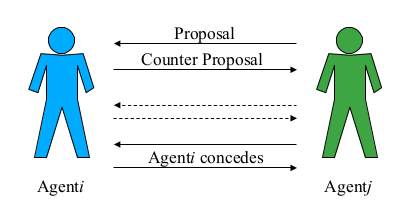
\includegraphics[width=.5\textwidth]{01/01}
\end{figure}

Another way of looking at the negotiation process is as an iterative concession process: each agent starts at its most preferred outcome and makes a proposal, it will then proceed to conceed to a less preferred outcome until a \side{Point of acceptance or agreement} is reached. (Be aware of the fact that not all negotiation end with agreement).

\begin{figure}[!h]
\centering
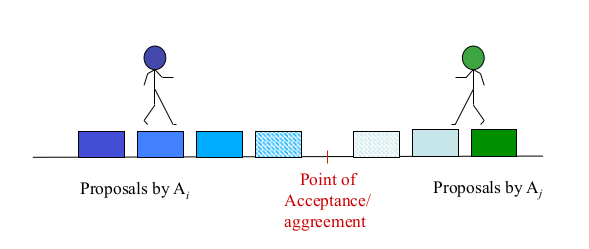
\includegraphics[width=.5\textwidth]{01/02}
\end{figure}

Hence the Negotiation process can be seen as moving towards a point of agreement.

\section{Multiagent Interactions}
	In the typical structure of a multiagent systems, one can notice the presence of some common elements:
	\begin{itemize}
	\item the system contains a number of agents
	\item each agent has the ability to communicate with another agent
	\item each agent has the ability to act in an environment
	\item different agents have different \side{spheres of influence}, i.e. they are able to influence or have control over the environment, or a part of it.
	\item these spheres of interest may coincide or overlap giving rise to dependencies between agents.
	\end{itemize}	
	
	Thus:\\
	\say{When faced with what appears to be a multiagent domain, it is critically important to understand the type of interaction that takes place between agents in order to be able to make the best decision possible about what action to perform.}

\subsection{Utilities and Preferences}
In order to simplify the analysis of multiagent interactions, throughout this chapter we will consider the following assumption, unless stated differently:
	\begin{itemize}
	\item Two agents act and interact in an environment. We will refer to these two agents as agent $i$ and agent $j$
	\item The two agents are \side{self-interest}, i.e. each agent has its own preferences and desires about how the world should be
	\item There exists a \side{set of outcomes} that the two agents have preferences over. We will refer to this set with the notation:
	\[\Omega = \{\omega_1, \omega_2,...\}\]
	\end{itemize}
	
	The preferences of the two agents are formally captured by means of \side{utility functions}, which maps each outcome in the set $\Omega$ to a real number describing how “good” an outcome is.\\
	Since the agents are self-interest each agent will have its own utility function, hence:
	\[u_i\,:\,\Omega\rightarrow\mathbb{R}\qquad;\qquad u_j\,:\,\Omega\rightarrow\mathbb{R}\]
	The introduction of an utility function eventually leads to a \side{preference ordering} over the outcomes of the set for each agent.
	This means that, if $\omega$ and $\omega’$ are both possible outcomes contained in $\Omega$ and $u_i(\omega)\ge u_i(\omega’)$, then agent $i$ prefers outcome $\omega$ at least as much as outcome $\omega’$.
	
	Since we will make extensive use of the concept of preference ordering throughout the next sections, it is worth introduce a much more compact notation. We will write:
	\begin{align*}
	\omega \cge_i \omega’ &&\text{ as an abbreviation for } && u_i(\omega) \ge u_i(\omega’)\\
	\omega \cmore_i \omega’ &&\text{ as an abbreviation for } && u_i(\omega) > u_i(\omega’)
	\end{align*}
	where the second expression represents the case in which outcome $\omega$ is \side{stricly preferred} by agent $i$ over $\omega’$.
	
	In other words, the notation can be summarized as follows:
	\begin{empheq}[box=%
	\fbox]{gather*}
		\omega \cmore_i \omega’ \,\iff\,u_i(\omega)\ge u_i(\omega’)\text{ and not } u_i(\omega)=u_i(\omega’)
	\end{empheq}
	
	Moreover we can notice that the ordering relation expressed by the operator $\cge$, has the following properties:
	\begin{enumerate}
	\item \side{Reflexivity}
	\[\forall \omega \in \Omega\rightarrow \omega\cge_i\omega\]
	\item \side{Transitivity}
	\[\text{If } \omega \cge_i\omega’ \text{ \&\& } \omega’\cge_i\omega`` \rightarrow \omega \cge_i\omega``\]
	\item \side{Comparability}
	\[\forall \omega\in \Omega, \forall \omega’\in\Omega\rightarrow \omega\cge_i\omega’\text{ || } \omega’\cge_i\omega\]
	\end{enumerate}
	The strict preference relationship still has the second and third property, however it is not reflexive
	
\subsection{Setting the scene}
So far, we have introduced a model to represent the agents preferences, but we still need to formalize a model of the environment in which agents act and interact. In particular, we will assume that:
	\begin{itemize}
	\item Two agents will simultaneously choose an action to perform in the environment
	\item as a result of the actions they select, an outcome in $\Omega$ will result
	\item the \side{actual outcome} that will result will depend on the particular \side{combination of actions} performed.
	
	In other terms: both agents can influence the actual outcome 
	\item The two agents must perform an action
	\item The two agents cannot see the action performed by the other agent
	\end{itemize}
	
	We will restrict our analysis to two possible actions that the agent can choose from: cooperate $C$ and defect $D$. Hence, we will refer to the \side{set of actions} with the notation
	\[Ac = \{C,D\}\]
	Given all the above, the environment is formally described by a \side{state transformer function}:
	\[\tau: \underbrace{Ac}_{\text{agent $i$’s action}}\times\underbrace{Ac}_{\text{agent $j$’s action}}\rightarrow \Omega\]
	Hence, several scenarios can happen:
	\begin{enumerate}
	\item The environment maps each combination of actions to a different outcome, and thus is sensitive to the actions of both agents
	\[\tau(D,D)=\omega_1\qquad\tau(D,C)=\omega_2\qquad\tau(C,D)=\omega_3\qquad\tau(C,C)=\omega_4\]
	\item The environment maps each combination of actions to the same outcome and thus neither of the agents have influence in the environment
	\[\tau(D,D)=\omega_1\qquad\tau(D,C)=\omega_1\qquad\tau(C,D)=\omega_1\qquad\tau(C,C)=\omega_1\]
	\item The environment maps each combination of actions to an outcome that is correlated to the choice of only one agent and thus the outcome depends solely on the action performed by one agent
	\[\tau(D,D)=\omega_1\qquad\tau(D,C)=\omega_2\qquad\tau(C,D)=\omega_1\qquad\tau(C,C)=\omega_2\]	
	\end{enumerate}
	Since the latter two cases are of no interest for our analysis we will focus on the scenario in which both agents exert some kind of influence on the actual outcome. We, therefore, will consider the agent preferences (in the form of utility function) as follows
	\[
	\left.
	\begin{aligned}
	u_i(\omega_1) = 1&\quad u_i(\omega_2) = 1&\quad u_i(\omega_3) = 4&\quad u_i(\omega_4) = 4\\
	u_j(\omega_1) = 1&\quad u_j(\omega_2) = 4&\quad u_j(\omega_3) = 1&\quad u_j(\omega_4) = 4
	\end{aligned}
	\right\}
	\]
	Given the state transformer function, we can abuse notation and write
	\[
	\left.
	\begin{aligned}
	u_i(D,D) = 1&\quad u_i(D,C) = 1&\quad u_i(C,D) = 4&\quad u_i(C,C) = 4\\
	u_j(D,D) = 1&\quad u_j(D,C) = 4&\quad u_j(C,D) = 1&\quad u_j(C,C) = 4
	\end{aligned}
	\right\}
	\]
	Hence, with respect to agent $i$’s preferences (first row) over the possible outcomes, we can characterize the preference ordering as follows:
	\[(C,C) \cge_i(C,D) \cge_i(D,C) \cge_i(D,D) \]
	Similarly for agent $j$, the resulting preference ordering can be characterize as follows:
	\[(C,C) \cge_i(D,C) \cge_i(C,D) \cge_i(D,D) \]
	It is straightforward to see that if both agents \side{act rationally}, i.e. \say{they both choose to perform the action that will lead to their preferred outcomes}\cite{mastxt}, they will both choose to cooperate.
	This is because, both agents prefer all the outcomes in which they cooperate, regardless of what the other agent action is.
	
	A common way to represent the previously described interaction scenario is via \side{pay-off matrix} (standard game-theoretic notation):
	\begin{table}[!h]
	\centering
	\begin{NiceTabular}{c|w{c}{0.75cm}w{c}{0.75cm}|w{c}{0.75cm}w{c}{0.75cm}}
	&\Block{1-2}{i defects}&&\Block{1-2}{i cooperates}&\\
	\hline
	\Block{2-1}{j defects}&&1&&4\\
	&1&&1&\\
	\hline
	\Block{2-1}{j cooperates}&&1&&4\\
	&4&&4&
	\end{NiceTabular}
	\end{table}
	The pay-off matrix uniquely defines a \side{game in strategic form}. The way to interpret it is as follows:
	\begin{itemize}
	\item each cell in the matrix correspond to one of the possible outcomes
	\item The top-right value in each cell corresponds to the payoff received by the column player
	\item The bottom-left value in each cell corresponds to the payoff received by the row player
	\end{itemize}
	
\subsection{Solution Concepts and Solution Properties}
A question still remains unanswered: What should an agent do? What action should it choose? 
		
		We briefly touched on the topic on the previous section, but we have provided neither the concepts that make up the solution nor the desirable properties that a solution should have.
		
		In this section, we will tackle the problem to its core.
		
\subsubsection{Dominant strategies - Dominance}
One of the main concept that we will introduce is that of \side{dominance}.
		
		\say{A strategy $s_i$ is [said to be] \textbf{dominant} for player $i$ if, no matter what strategy $s_j$ agent $j$ chooses, $i$ will do at least as well playing $s_i$ as it would doing anything else}\cite{mastxt}.
		The notion of \side{dominant strategy} is strictly related to the concept of \side{best response}, in the sense that \say{a strategy $s_i$ for agent $i$ is dominant if it is the best response to \textbf{all} of agent $j$ strategies}\cite{mastxt}.
		
		Thus, a dominant strategy, if it exists, simplify the decision about what action to perform: \say{the agent guarantees its best outcome 
by performing the dominant strategy}\cite{mastxt}.

\subsubsection{Nash Equilibria}
The notion of \side{equilibrium}, or more precisely \side{Nash equilibrium}, is hard to formalize in the context of strategic decision making.
		
		We can, however, provide a basic definition by saying that two strategies $s_1$ and $s_2$ are in Nash equilibrium if:
		\begin{enumerate}
		\item under the assumption that agent $i$ plays $s_1$, agent $j$ can do no better than play $s_2$, and
		\item under the assumption that agent $j$ plays $s_2$, agent $i$ can do no better than play $s_1$
		\end{enumerate}
		From this conditions, one can clearly notice that \textbf{two strategies are in Nash equilibrium if they are the best response to each other}.
		
		The mutual nature of the concept makes it so that \emph{neither agent has any incentive to deviate from a Nash equilibrium}: even if an agent chooses a different strategy, the other agent can do no better than to choose the strategy in Nash equilibrium.
		
		Technically, this type of Nash equilibrium is known as \side{pure strategy Nash equilibrium}, and as much as it is appealing from its theoretical stand point, it is extremely expensive from a computational stand point.\\
		In fact, finding one or more Nash equilibria requires to consider each combination of strategy and check if they are in Nash equilibrium.\\
		Thus, if there are $n$ agents, each with $m$ possible strategies to choose from, the number of possible combinations of actions (and hence possible outcomes) will be $m^n$.
		
		Nonetheless, the presence of Nash equilibrium provides a definite answer to what action an agent should choose. However, two common issues might emerge:
		\begin{enumerate}
		\item Not every interaction scenario has a pure strategy Nash equilibrium
		\item Some interaction scenarios have more than one pure strategy Nash equilibrium
		\end{enumerate}
		
		With regard to the first issue, we need to modify our notion of what a strategy is. So far, we have implicitly considered a strategy as a deterministic choice of an action. This is inline with the fact that the subroutines that an agent can execute should not be subject to uncertainties or randomness (in general, we would like a subroutine to yield the same correct result on different execution).
		
		However, \say{it can be useful to introduce randomness or uncertainty into our actions}\cite{mastxt}.
		The reason why that is can be best explained considering the game or rock-paper-scissors, of which the pay-off matrix is provided below:
		\begin{table}[!h]
		\centering
		\begin{NiceTabular}{c|w{c}{0.75cm}w{c}{0.75cm}|w{c}{0.75cm}w{c}{0.75cm}|w{c}{0.75cm}w{c}{0.75cm}}
		&\Block{1-2}{i plays rock}&&\Block{1-2}{i plays paper}&&\Block{1-2}{i plays scissors}&\\
		\hline
		\Block{2-1}{j plays rock}&&0&&1&&-1\\
		&0&&-1&&1&\\
		\hline
		\Block{2-1}{j plays paper}&&-1&&0&&1\\
		&1&&0&&-1&\\
		\hline
		\Block{2-1}{j plays scissors}&&1&&-1&&0\\
		&-1&&1&&0&
		\end{NiceTabular}
		\end{table}
		From the provided payoff matrix, one can clearly notice that the game has no pure strategy Nash equilibrium as well as no dominant strategy.
		Yet, this is not completely true: a \side{mixed strategy} allows the agent to choose between possible choices by introducing randomness into the selection.\\
		If the agent chooses one of the actions at random, with each choice having equal probability of being selected, the strategy turns out to be in \textbf{Nash equilibrium with itself}. This is because if an agent decides to choose an action at random, the other agent can do no better than adopting the same strategy and vice versa.
		
		In general, if a player has $k$ possible choices, $s_1, s_2, ..., s_k$, then a mixed strategy over these choices takes the form:
		\begin{itemize}
		\item play $s_1$ with probability $p_1$
		\item play $s_2$ with probability $p_2$
		\item ...
		\item play $s_k$ with probability $p_k$
		\end{itemize}
		In other terms, a mixed strategy over $s_1, s_2, ..., s_k$ is a probability distribution over $s_1, s_2, ..., s_k$.
		
		The result formalized by John Forbes Nash, Jr. best summarize the discussion that we have made so far:\\
		\say{Every game in which every player has a finite set of possible strategies has a Nash equilibrium in mixed strategies}
		
\subsubsection{Pareto efficiency}
The notion of \side{Pareto efficiency} or \side{Pareto optimality}, contrary to the notion of Nash equilibrium and dominant strategy, is more of a (desirable) property of solutions rather than a solution concept.
		
		Formally:\\
		\say{an outcome is Pareto efficient if there is no other outcome that improves one player’s utility without making somebody else worse off}.\cite{mastxt}\\
		On the other hand:
		\say{An outcome is said to be Pareto inefficient if there is another outcome that makes at least one player better off without making anybody else worse off}\cite{mastxt}.
		
		To put it in simpler terms we can consider an example: a brother and a sister have to divide a cake. Among the solutions of this problem, those who are Pareto efficient are:
		\begin{itemize}
		\item The brother eats the whole cake
		\item The sister eats the whole cake
		\item Any other distribution of the cake, which leaves no cake left
		\end{itemize}
		Hence, a solution is Pareto efficient if it consumes/uses the total utility.
		
\subsubsection{Maximizing social welfare}
Similarly to Pareto efficiency, \side{social welfare} is an important property of outcomes, but is not generally a way of directly selecting them.
		
		The core principle of \side{Maximizing social welfare} involves the measurement of how much utility is created by an outcome in total.\\
		Formally, let $sw(\omega)$ denote the sum of utilities of each agent for outcome $\omega$
		\[sw(\omega) =\sum_{i\in Ag} u_i(\omega)\]
		the outcome that maximizes social welfare is the one that maximizes this value.
		
		From an individual agent’s point of view, the problem with maximizing social welfare is that it does not look at the pay-offs of individual agents, only to the total welfare created. (maximizing social welfare does not care about how the utility of an outcome is divided among the players).


\subsubsection{Other minor properties}
\begin{itemize}
\item \side{Convergence/ guaranteed success}\\
If it ensures that eventually agreement is certain to be reached.
\item \side{Computational efficiency}\\
As little computations is needed as possible. Trade off between the cost of the process and the solution quality
\item \side{Distribution}\\
All else being equal, distributed protocols should be preferred to avoid a single point of failure and a performance bottleneck. This may conflict with minimizing the amount of communication that is required.
\item \side{Stability}\\
Among self interested agents, mechanism should be designed to be stable (non-manipulable), it should motivate each agent to behave in the desired manner.
\item \side{Individual rationality}\\
Participation in a negotiation is individually rational to an agent if the agent's payoff in the negotiated solution is no less than payoff that the agent would get by not participating in the negotiation.\\
A mechanism is individually rational if participation is individually rational for all agents.\\
If the negotiated solution is not individually rational for some agent then self-interested agent would not participate in that negotiation.
\end{itemize}
\subsection{Competitive and Zero-Sum Interactions}
A scenario in which an outcome $\omega\in\Omega$ is preferred by agent $i$ over an outcome $\omega’$, if, and only if, $\omega’$ is preferred over $\omega$ by agent $j$, is said to be \side{strictly competitive}.\\
	Formally, a competitive scenario takes the form:
	\[\omega \cmore_i \omega’\qquad\iff\qquad\omega’\cmore_j \omega\]
	Under this condition, it is straightforward to see that the preferences of the players are \side{diametrically opposed} to one another
	
	\side{Zero-sum encounters}, similarly, are those in which, for any particular outcome, the utilities of the two agents sum to zero. Formally, these scenario is described by the condition:
	\[u_i(\omega) + u_j(\omega) = 0\qquad \forall \omega \in \Omega\]
	Once again, any zero-sum scenario is strictly competitive, allowing for no possibility of cooperative behavior: \say{the best outcome for an agent is the worst outcome for its opponent. If an agent allows the opponent to get a positive utility, then it will get negative utility.}\cite{mastxt}\\
	Popular Zero-sum encounters are the games of chess and checkers as well as rock-paper-scissors.
	
	Interesting enough, it is debatable that zero-sum games actually exists in real-world scenarios (apart from artificially forms of interaction like the games mentioned before). However, it appears that people interacting in many scenarios have a tendency to treat them as if they were zero sum.
	
\subsection{The Prisoner's Dilemma}
The \side{Prisoner’s Dilemma} is as follows:
	\say{Two man are collectively charged with a crime and held in separate cells. They have no way of communicating with each other or making any kind of agreement. The two man are told that:
	\begin{enumerate}
	\item If one of them confesses to the crime and the other does not, the confessor will be freed, and the other will be jailed for three years
	\item If both confess to the crime, then each will be jailed for two years
	\end{enumerate}
	Both prisoners know that if neither confesses, then they will each be jailed for one year.}\cite{mastxt}
	Under this conditions let us associate the act of confessing with defection $D$ and not confessing with cooperating $C$.
	
	There exists 4 possible outcomes to the prisoner’s dilemma:
	\begin{table}[!h]
	\centering
	\begin{NiceTabular}{c|w{c}{0.75cm}w{c}{0.75cm}|w{c}{0.75cm}w{c}{0.75cm}}
	&\Block{1-2}{i defects}&&\Block{1-2}{i cooperates}&\\
	\hline
	\Block{2-1}{j defects}&&2&&0\\
	&2&&5&\\
	\hline
	\Block{2-1}{j cooperates}&&5&&3\\
	&0&&3&
	\end{NiceTabular}
	\end{table}
	
	Where the number displayed are NOT the year spent in prison.
	
	From the provided payoff matrix we can come up with the preference ordering of each agent/prisoner:
	\[
	\begin{dcases}
	(D,C) \cmore_i (C,C) \cmore_i (D,D) \cmore_i (C,D) & \text{for agent }i\\
	(C,D) \cmore_j (C,C) \cmore_j (D,D) \cmore_j (D,C) & \text{for agent }j\\
	\end{dcases}
	\]
	Thus, we can analyze the best response of an agent to the choice of action of the other:
	\begin{itemize}
	\item Assuming the other player cooperates. The best response is to defect
	\item Assuming the other player defect. The best response is to defect
	\end{itemize}
	From this we can conclude that defection for $i$ is the best response to all possible strategies of the player $j$: by definition, defection is thus a dominant strategy for $i$.
	
	Since the same conclusion can be drawn for agent $j$, the scenario under consideration is \side{symmetric}: this will result in both agent choosing to defect.\\
	From an analysis of the problem under the concepts that we have seen previously, we can state that
	\begin{itemize}
	\item the pair $(D,D)$ is the only Nash equilibrium of the scenario, however intuition says that this is not the best the players can do. 		\item the pair of actions $(D,D)$ is also the only one that is not Pareto efficient. 
	\item The outcome that maximizes social welfare is $(C,C)$
	\end{itemize}
	
	\say{The fact that utility seems to be wasted here, and that the agents could both do better by cooperating, even though the rational thing to do is to defect, is why this is referred to as dilemma.} \cite{mastxt}
	
	Moreover, the prisoner’s dilemma also seems to be the game that characterized the \side{tragedy of the commons}: which is concerned with the use of a shared, depletable resource by a society of self-interested individuals (e.g. overfishing in the seas, exploitation of bandwidth capacity on the Internet).
	
	Many people find the conclusion of the analysis deeply upsetting: \say{the result seems to imply that cooperation can only arise as a result of irrational behavior, and that cooperative behavior can be exploited by those who behave rationally.}\cite{mastxt}\\
	Binmore argues that the discomfort we have with the analsys of the prisoner’s dilemma is misplaced:\\
	\say{A whole generation of scholars swallowed the line that the prisoner’s dilemma embodies the essence of the problem of human cooperation. They therefore set themselves the hopeless task of giving reasons why [this analysis] is mistaken... Rational players don’t cooperate in the prisoner’s dilemma because the conditions necessary for rational cooperation are absent}.
	
\subsection{Other Symmetric 2$\times$2 Interactions}
The prisoner’s dilemma and its variation are not the only type of multiagent interaction that exists.
	
	In fact, if we restrict our attention to interaction in which there are:
	\begin{itemize}
	\item Two agents
	\item Each agent has two possible actions (C or D)
	\item The scenario is symmetric
	\end{itemize}
	Then $4! = 24$ possible orderings of preferences, and as a consequence, 24 different games, can be constructed.
	
	\begin{table}[!h]
	\centering
	\begin{NiceTabular}{lll}[hvlines]
	\textbf{Scenario}&\textbf{Preferences over outcomes}&\textbf{Comment}\\
	1&$(C,C)\cmore_i(C,D)\cmore_i(D,C)\cmore_i(D,D)$&cooperation dominates\\
	2&$(C,C)\cmore_i(C,D)\cmore_i(D,D)\cmore_i(D,C)$&cooperation dominates\\
	3&$(C,C)\cmore_i(D,C)\cmore_i(C,D)\cmore_i(D,D)$&\\
	4&$(C,C)\cmore_i(D,C)\cmore_i(D,D)\cmore_i(C,D)$&stag hunt\\
	5&$(C,C)\cmore_i(D,D)\cmore_i(C,D)\cmore_i(D,C)$&\\
	6&$(C,C)\cmore_i(D,D)\cmore_i(D,C)\cmore_i(C,D)$&\\
	7&$(C,D)\cmore_i(C,C)\cmore_i(D,C)\cmore_i(D,D)$&\\
	8&$(C,D)\cmore_i(C,C)\cmore_i(D,D)\cmore_i(D,C)$&\\
	9&$(C,D)\cmore_i(D,C)\cmore_i(C,C)\cmore_i(D,D)$&\\
	10&$(C,D)\cmore_i(D,C)\cmore_i(D,D)\cmore_i(C,C)$&\\
	11&$(C,D)\cmore_i(D,D)\cmore_i(C,C)\cmore_i(D,C)$&\\
	12&$(C,D)\cmore_i(D,D)\cmore_i(D,C)\cmore_i(C,C)$&\\
	13&$(D,C)\cmore_i(C,C)\cmore_i(C,D)\cmore_i(D,D)$&game of chicken\\
	14&$(D,C)\cmore_i(C,C)\cmore_i(D,D)\cmore_i(C,D)$&prisoner’s dilemma\\
	15&$(D,C)\cmore_i(C,D)\cmore_i(C,C)\cmore_i(D,D)$&\\
	16&$(D,C)\cmore_i(C,D)\cmore_i(D,D)\cmore_i(C,C)$&\\
	17&$(D,C)\cmore_i(D,D)\cmore_i(C,C)\cmore_i(C,D)$&\\
	18&$(D,C)\cmore_i(D,D)\cmore_i(C,D)\cmore_i(C,C)$&\\
	19&$(D,D)\cmore_i(C,C)\cmore_i(C,D)\cmore_i(D,C)$&\\
	20&$(D,D)\cmore_i(C,C)\cmore_i(D,C)\cmore_i(C,D)$&\\
	21&$(D,D)\cmore_i(C,D)\cmore_i(C,C)\cmore_i(D,C)$&\\
	22&$(D,D)\cmore_i(C,D)\cmore_i(D,C)\cmore_i(C,C)$&\\
	23&$(D,D)\cmore_i(D,C)\cmore_i(C,C)\cmore_i(C,D)$&defection dominates\\
	24&$(D,D)\cmore_i(D,C)\cmore_i(C,D)\cmore_i(C,C)$&defection dominates
	\end{NiceTabular}
	\end{table}

	For the sake of the analysis we will briefly look into two more of these games: stag hunt and the game of chicken.

\begin{itemize}
\item The stag hunt
\begin{table}[!h]
	\centering
	\begin{NiceTabular}{c|w{c}{0.75cm}w{c}{0.75cm}|w{c}{0.75cm}w{c}{0.75cm}}
	&\Block{1-2}{i defects}&&\Block{1-2}{i cooperates}&\\
	\hline
	\Block{2-1}{j defects}&&1&&0\\
	&1&&2&\\
	\hline
	\Block{2-1}{j cooperates}&&2&&3\\
	&0&&3&
	\end{NiceTabular}
	\end{table}
	
\item The Game of chicken
\begin{table}[!h]
	\centering
	\begin{NiceTabular}{c|w{c}{0.75cm}w{c}{0.75cm}|w{c}{0.75cm}w{c}{0.75cm}}
	&\Block{1-2}{i defects}&&\Block{1-2}{i cooperates}&\\
	\hline
	\Block{2-1}{j defects}&&0&&1\\
	&0&&3&\\
	\hline
	\Block{2-1}{j cooperates}&&3&&2\\
	&1&&2&
	\end{NiceTabular}
	\end{table}
\end{itemize}	


\section{Voting}
So far we have looked at the general setting of a multiagent encounter. In this section we will look at a specific class of protocols intended for making group decisions. This is the domain of social choice theory (aka voting theory).

\subsection{Social Welfare Functions and Social Choice Functions}
The general setting of a voting protocol is as follows:
\begin{itemize}
\item A set of agents or \side{voters}
\[Ag = \{1, ...,n\}\]
Ideally, this should be finite and the cardinality should be an odd number to avoid ties.
\item A set of possible outcomes or \side{candidates}
\[\Omega =\{\omega_q, \omega_w, ...\}\]
over which voters will make group decision. This set is assumed to be finite.

The goal of the agents is to rank or order these candidates or simply to choose one from the set.
\end{itemize}
The problem that social choice theory tries to solve is,\\
 \say{given a collection of preference orders, one for each agent, how do we combine these to derive a group decision?}.
 
 The answer is by using a \side{social welfare function} which maps the voter preferences to a \side{social preference order}\\
 \[f:\quad \Pi(\Omega) \times ...\times\Pi(\Omega) \rightarrow \Pi(\Omega)\]
 The social preference ordering will be denoted with the notation $\cmore^*$.
 
 If the agents are required to choose just one candidate over the set $\Omega$, we will use a \side{social choice function} or \side{voting procedure}:
 \[f:\quad \Pi(\Omega) \times ...\times\Pi(\Omega) \rightarrow \Omega\]

\subsection{Voting Protocols}
\subsubsection{Simple majority voting}
\begin{itemize}
\item Every voter submits their preference order
\item The winner is the outcome that appears first in the preference orders the largest number of times
\item This is generally applied to single choice, but it can be generalized to a social preference ordering.
\end{itemize}
\phantom{c}\side{Simple majority voting} works relatively well with only two candidates, since it is straightforward to implement and understand by the voters.

However, when more than 2 voters are involved problems start to arise.

Let us consider that three voters submitted the following preferences:
\begin{align*}
42\%\qquad& \omega_L \cmore \omega_D \cmore \omega_C\\
14\%\qquad& \omega_D \cmore \omega_L \cmore \omega_C\\
44\%\qquad& \omega_C \cmore \omega_D \cmore \omega_L\\
\end{align*}
Then the winner is selected based on the top preferences (i.e. $C$), even though the majority of the voters considered $C$ as the least preferrable outcome.

This means that in principle the majority of the voters will be unhappy with the result of the voting protocol.

Furthermore, this simple majority protocol is sensible to insincere strategical voting (e.g. the 14\% that voted $D$ instead could have voted for $L$ just to make $C$ lose the voting).

Moreover, the simple majority voting is sensible to \side{Condorcet's paradox}:
\begin{gather*}
\omega_1 \cmore_i \omega_2 \cmore_i \omega_3\\
\omega_3 \cmore_j \omega_1 \cmore_j \omega_2\\
\omega_2 \cmore_k \omega_3 \cmore_k \omega_1\\
\end{gather*}
In this case the winner is dependent on the agenda: which order we start to compute the outcome, but nonetheless $\sfrac{2}{3}$ of the voters will prefer another candidate.

\subsubsection{Binary protocol}
Among the alternative to simple majority voting there is the \side{Binary protocol} (aka sequential majority elections).

\begin{itemize}
\item Voters submit their preference ordering
\item The element of the set of outcomes are compared pairwise
\item the winner of the pairwise ``election'' is allowed to continue to the next pairwise election
\item The order of pairwise elections (i.e. which candidates to compare first), is called \side{agenda}
\end{itemize}

\begin{figure}[!h]
\centering
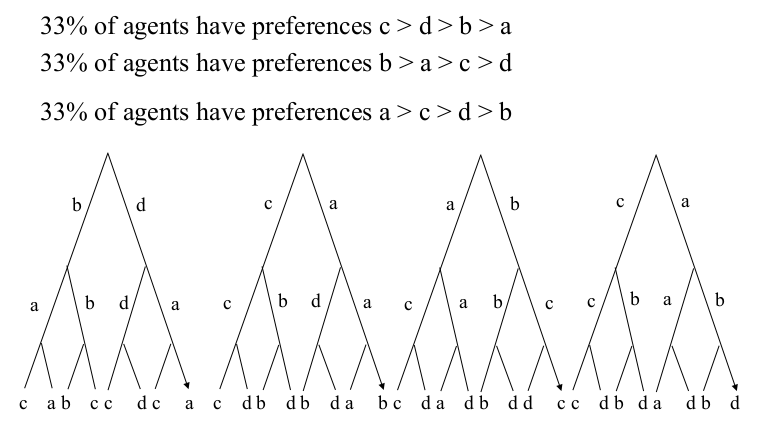
\includegraphics[width= .5\textwidth]{01/03}
\end{figure}


From the picture provided we can clearly notice that the winner of the overall election depends on the agenda, which imply that the protocol can be manipulated if the preference orderings in known a priori.

\subsubsection{Borda protocol}
One issue with simple majority voting and the binary protocol is that they completely ignore the information that is enconded in each submitted preference ordering (they only look at the top voted candidates).\\
The \side{Borda protocol} addresses such issue:
\begin{itemize}
\item Each voter submit its preference ordering over the candidates
\item a number equal to the cardinality of the set of candidates (i.e. $\abs{\Omega}$) is assigned to the highest candidate in some agent's preference list
\item a value of $\abs{\Omega}-1$ is assigned to the second and so on
\item a the end we sum up the numeric value associated to each preference ordering and obtain the social choice result
\end{itemize}

This protocol is fast when compared to the binary protocol in the case of a large amount of candidates.

However it is not  \side{indipendent of irrelevant alternatives}, i.e. removing one candidate will change the end result.


\subsubsection{Majority Graph: Condorcet's Winner and Slater ranking}
An useful tool to analyse voting procedures or protocols is the \side{Majority Graph}. It can be considered as a succint representation of the voter preferences:
\begin{itemize}
\item each node in the majority graph is a candidate
\item each edge in the majority graph represents a preference (the edge will start from the node most preferred and will terminate in the node less preferred)
\item a \side{possible winner} is a candidate that is the overall winner for at least one agenda. (occurs when there are loops in the majority graph)
\item a \side{Condorcet's winner} is a candidate that is the overall winner for all possible agenda (occurs when there are no loops in the majority graph). In simple terms, is that candidate that will beat all others in a pairwise election.
\end{itemize}

While the overall winner determination is straightforward in the case of a majority graph with no loops (cfr. Condorcet's Winner), it is otherwise in the case of a majority graph with loops.

In that specific scenario, the \side{slater rule} or \side{slater ranking} is considered: it, in fact, tries to find a consistent ranking that does not contain any cycle that is as close as possible to the majority graph.

In other terms, it tries to \say{minimize the number of disagreements between the majority graph and the social choice}.

In practice, the Slater ranking considers the Condorcet's winners obtained by inverting the least amount of edges in the majority graph.
\subsection{Desirable Properties for Voting Procedures}
\begin{enumerate}
\item \side{Pareto condition}\\
There is no other outcome that makes one agent better off without making another agent worse off.

Borda and simple majority voting satisfy this condition.\\
Binary protocol does not (the result depends on the agenda).
\item \side{Condorcet winner condition}\\
The Condorcet winner should be selected by the social choice function.

Only Binary protol satisfies this condition.
\item \side{Indipendence of irrelevant alternatives}\\
Given a set of candidates of which $\omega_i$ and $\omega_j$ are part of. \\
Let us assume that $\omega_i \cmore^* \omega_j$.\\
A change in preferences in any other candidate should not change the relative ranking of $\omega_i$ and $\omega_j$.

None of the protocol we have seen satisfies this property.
\item \side{Dictatorship}\\
A social welfare function is said to be a dictatorship if for some voter $i$ we have
\[f(\bar{\omega_1}, \bar{\omega_2}, ...) = \bar{\omega_i}\]

All protocols we have seen so far are non-dictatorship.
\end{enumerate}

\begin{theorem}[Arrow's theorem]\pside{Arrow's theorem}\\
If $\abs{\Omega}>2$ then the only voting procedure that satisfies Pareto condition, Condercet Winner condition and IIA is dictatorship.
\end{theorem}
\subsection{Insincere Voters}
\begin{itemize}
\item In reality it is seldom that all agent's preferences are known: usually agents have to reveal their preferences.
\item Assuming knowledege of the preferences is equivalent to assuming that the agents reveal their preferences truthfully
\item If an agent can benefit from insincerely declaring his preferences, it will do so.
\item The goal is to generate protocols such that when agents use them according to some stability solution concept (dominant strategy equilibrium) the desirable social outcomes follow
\item The strategies are not externally imposed on the agents, but instead each agent uses the strategy that is best for itself
\end{itemize}
However:\\

Let each agent $i$ from $A$ have some ordering $\theta_i$ from $\Theta$ which totally characterizes his preferences. A social choice function $f:\quad \Theta \rightarrow \Omega$ chooses a social outcome given the agent's orderings.

\begin{theorem}[Gibbard-Satterthwaite impossibility theorem]\pside{Gibbard- Satterthwaite impossibility theorem}\\
Let each agent's ordering $\theta_i$ consists of a preference order $\cmore_i$ on $\Omega$.\\
Let there be no restictions on $\cmore_i$ (i.e. each agent may rank the outcomes $\Omega$ in any order).\\
Let $\abs{\Omega} > 2$.\\
Now, if the social function $f(\cdot)$ is truthfully implementable in a dominant strategy equilibrium (or is not manipulable), then $f(\cdot)$ is dictatorial, i.e. there is some agent who gets one of its most preferred outcome chosen no matter what types the other reveal.
\end{theorem}

Broadly speaking, the only procedure or mechanism that is immune to strategic manipulation (in the sense of untruthful report of an agent preference) is dictatorship in the case of more than 2 candidates.

There are ways to circumvent the impossibility theorem, by relaxing the assumptions made by the theorem itself.\\
The individual preferences, in fact, may happen to belong to some restrincted domain, thus invalidating the conditions of the impossibility theorem, and it is known that there are island in the space of agent's preferences for which non-manipulable non-dictatorial protocols can be constructed.

The solution in practice is to make agents precisely internalize the externality by imposing a tax on those agents whose vote changes the outcome. The size of tax is exactly how much its vote lowers the other's utility.\\
Such solution is known as the \side{Clark tax algorithm}:
\begin{itemize}
\item Every agent $i$ from $A$ reveals his valuation $v^*_i(g)$ for every possible $g$ (which may be non-truthful)
\item The social choice is 
\[g^* =\argmax_g \, \sum \,v^*_i(g)\]
\item Every agent is levied a tax:
\[tax_i = \sum_{j\ne i} v^*_j\,\left(\argmax_g\, \sum _{k\ne i}\,v^*_k(g)\right) - \sum_{j\ne i}\,v^*_j(g)\]
\end{itemize}
It follows that
\begin{theorem}
If each agent has quasilinear preferences, then, under the Clarke tax algorithm, each agent's dominant strategy is to reveal his true preferences, i.e. 
\[v^*_i(g) = v_i(g) \qquad\forall g\]
\end{theorem}

In conclusion, the Clarke tax algorithm:
\begin{itemize}
\item the mechanism leads to the socially most preferred $g$ to be chosen
\item because of truth telling, the agents need not waste effort in counter speculating each other preference declarations
\item participation in the mechanism may only increase an agent's utility
\item the mechanism does not mantain budget balance: too much tax is collected
\item it is not coalision proof 
\end{itemize}

Other way to circumvent the Impossibilty theorem:
\begin{itemize}
\item some fairness can be achieved by choosing the dictator randomly in the protocol
\item to use a protcol for which computing an untruthful revelation (that is the better than the truthful one) is prohibitively costly computationally
\end{itemize}

\section{Auctions}
Auctions are mechanisms used to reach agreeements on one very simple issue: that of how to allocate scarce resources to agents.

It is important to understand that the resource in question is scarce and it is tipically desired by more than one agent (if one of the preconditions is not met than the allocation is trivial and straighforward).

Auctions provide a reasonable and principled way to allocate resources to agents, in particular they are effective at allocating resources efficiently, in the sense of allocating resources to those that value them the most.
\subsection{Auction parameters for classification}
In general terms:
\begin{itemize}
\item An auction takes place between an agent known as the \side{auctioneer} and a collection of agents known as the \side{bidders}
\item The goal of the auction is for the auctioneer to allocate a good to one of the bidders
\item The auctioneer desires to maximize the price at which the good is allocated.

Hence the agent auctioneer will attempt to achieve its desire through the design of an appropriate auction
\item The bidders desire to minimize the selling price.

Hence the bidder agents will attempt to achieve their desires by using an effective strategy
\end{itemize}

There are several factors that can affect both the auction protocol and the strategy that agents use:
\begin{itemize}
\item The good has a \side{private value}, \side{public/common value} or a \side{correlated value} (i.e. an agent valuation of the good depends partly on private factors and partly on other agents' valuations of it).
\item \side{winner determination}: who gets the good that the bidders are bidding for and how much do they pay.

In this setting, there are \side{first-price auctions} (the price goes to the highest bidder) and \side{second-price auctions} (the price goes to the highest bidder but it will pay the amount bid by the second highest bid)
\item Whether or not the bids made by the agents are known to each other.

In this setting, we will  differentiate between \side{open-cry} and \side{sealed-bid}
\item The mechanism by which bidding proceeds.

In this setting, we will differentiate between \side{one shot}, \side{ascending auctions} or \side{descending auctions} (in which the price starts at a \side{reservation price}: in the case of ascending the reservation price is proposed by the first bidder, whereas in descending the reservation price is proposed by the auctioneer).
\end{itemize}
\subsection{English auctions}
English auctions are: first-price, open cry, ascending auctions.

\begin{itemize}
\item The auctioneer sets a reservation price for the good (low price) and the good is allocated to the auctioneer for this amount
\item Bids are then invited from agents, who must bid more than the current highest bid. (all agents can see the bid)
\item When no agent is willing to raise the bid, then the good is allocated to the agent that has made the current highest bid at the amount of its bid.
\end{itemize}

The dominant strategy is to bid a small amount more than the current highest bid until the bid price reaches their private valuation and then to withdraw.

English auction's however are sensible to the \side{winner's curse}: should the winner feel ``happy'' that they have obtained the good for less than or equal to their private valuation or should they feel worried because no other agent valued the good so highly?

\subsection{Japanese auctions}
Japanese auctions are: open cry, ascending auctions
\begin{itemize}
\item The auctioneer sets a reservation price
\item Each agent must choose whether or not to be in
\item The auctioneer successively increases the price
\item After each increase an agent must say if he stays or not. When agent drops out it is irrevocable
\item The auction ends when exactly one agent is left
\item The winner must buy the good for the current price
\end{itemize}

\subsection{Dutch auctions}
Dutch auctions are: open-cry, descending auctions:
\begin{itemize}
\item The auctioneer sets a reservation price
\item The auctioneer then continually lowers the offer price of the good by some small value, until some agent makes a bid for the good
\item The good is then allocated to the agent that made the offer
\end{itemize}
Dutch auctions are also susceptible to the winner's curse.

The dominant strategy is to shade bid a bit below the true willingness to pay.
\subsection{First-price sealed-bid auctions}
First-price sealed-bid auctions are: first-price, sealed-bid, one-shot auctions.
\begin{itemize}
\item A single round of proposals is considered
\item Bidders submit to the auctioneer a bid for the good
\item The good is awarded to the agent that made the highest bid
\item The winner pays the price of the highest bid
\end{itemize}
The dominant strategy for an agent is to bid less than it true valuation. How much less will of course depend on what the other agents bid (hence there is no general solution).

\subsection{Vickrey auctions}
Vickrey auctions are: second-price, sealed-bid auctions.
\begin{itemize}
\item There is a single bidding round
\item Each bidder submits a single bid.
\item The good is awarded to the agent that made the highest bid
\item The winning bidder pays the price of the second-highest bid 
\end{itemize}

The dominant strategy is truth telling: a bidder's dominant strategy in a private value Vickrey auction is to bid their true valuation. 

As such Vickrey auction are not prone to strategic manipulation, however it makes possible for \side{antisocial behaviour} to occur: one agent may bid close to the highest bid just to make the winner pay close to the amount that they have bid.
\subsection{Interralated auctions}
Some auctions are interralated to each other:
\begin{itemize}
\item Two good are sold separately, but the bidders would like to acquire them together
\item In this case the strategy to consider for more than one auction but for several interrelated auctions and then accomodate some valuations and  bids according to this strategy but not for some particolar auction. 
\end{itemize}

Let us consider the example of the proposed figure:

\begin{figure}[!h]
\centering
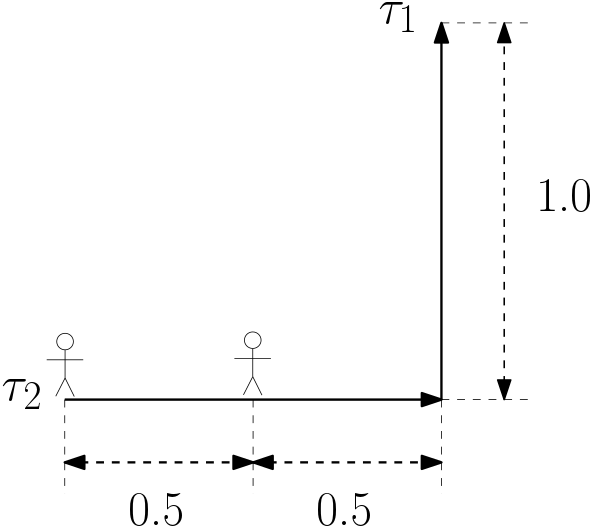
\includegraphics[width=.4\textwidth]{01/04}
\end{figure}

Two agents (agent 1 on the left and agent 2 on the right) are concurring for the acquisition of two tasks: $\tau_1$ and $\tau_2$.\\
It makes no sense for them to acquire just one of the two tasks. Please notice that in order to complete the full task an agent must go to the start of the arrow/task and fully traverse its edge.

Condering all of the above the valuation of the tasks for the two agents can be represented as a cost-to-go:

\begin{gather*}
\text{Agent 1: }\qquad c_1(\tau_1) =2.0 \qquad c_1(\tau_2) =1.0 \qquad c_1(\tau_1, \tau_2) =2.0\\
\text{Agent 2: }\qquad c_2(\tau_1) = 1.5  \qquad c_2(\tau_2) = 1.5 \qquad c_2(\tau_1, \tau_2) =2.5 
\end{gather*}
However if both agents decided to follow this strategy, task $\tau_1$ would go to agent 2 (lower cost to go), whereas task $\tau_2$ would go to agent 1 (lower cost to go).

In order for agent 1 to win both tasks, since it is of no use for an agent to win just one task in an interrelated auction, it can incorporate the full look ahead in its bid.

If in fact, agent 1 wins $\tau_1$, it will bid $c_1(\tau_2) = c_1(\tau_1, \tau_2) - c_1(\tau_1) = 0$ for the second task, otherwise it will bid $c_1(\tau_2) = 1$.
So it makes sense to accomodate the first bid with this knowledge.
If agent 1 wins $\tau_1$, it will win $\tau_2$ at the price of 0 and gets a payoff of $c_1(\tau_2) - 0 = 1$ that can redistribute to the first bid.

In conclusion the dominant strategy is to accomodate the payoff into the first bid:
\[c_1(\tau_1) -payoff = 2-1=1\]

In other terms this implies that if agent 1 realizes that by winning $\tau_2$ it will automatically win $\tau_1$, it will bid ``higher'' for $\tau_1$ or say that the effort to complete task $\tau_1$ will be lower by winning also  $\tau_2$. 

\subsection{Lies and Collusion}
It is in the auctioneer interest to have a protocol that is immune to collusion by bidders, i.e. that made it against the bidder' best interests to engage in collusion with other bidders.

Similarly, as a potential bidder in an auction, we would like a protocol that made honesty on the part of the auctioneer the dominant strategy.

None of the auction discussed above is immune to collusion: for any of them the grand coalition of all agents involved in bidding for the good can agree beforehand to collude to put forward artificially low bids for the good on offer.\\
When the good is obtaines, the bidders can then obtain its true value and split the profits among themselves.
A solution to collusion of the bidder is to modify the protocol so that the bidders cannot identify each other which however it's not possible in open cry auctions.

With regard to the honesty of the auctioneer, the main opportunity for lying occurs in the Vickrey auctions: the auctioneer can lie to the winner about the price of the second highest bid. A solution to this is to sign bids in some way so that the winner can independently verify the value of the second highest bid ro use a trusted third party to handle bids.

In open cry auction settings there is no possibility for lying by the auctioneer, nor in  the first-price sealed-bid auctions.

Lastly, another possible opportunity for lying by the auctioneer is to place bogus bidders (aka \side{shills}), in an attempt to artificially inflate the current bidding price.

Moreover, there are main limitation of auctions is that they are only concerned with the allocation of goods and as such are not adequate for settling agreements that concerns maters of mutual interest.

\section{Negotiation parameters}
The basic components that make up a negotiation setting are:
\begin{itemize}
\item A \side{Negotiation set}, which represents the space of possible proposals that agents can make
\item A \side{protocol}, which defines the legal proposals that agents can make, as a funciton of prior negotiation history.
\item A collection of \side{strategies}, one for each agent, which determine what proposals the agents will make.
\item A \side{rule} that determines when a deal has been struck, and what this agreement deal is.
\end{itemize}

Negotiation usually proceeds in a series of rounds, with some proposal made at every round. The proposals that agents make are defined by their strategy, must be drawn from the negotiation set, and must be legal, as defined by the protocol.\\
If agreement is reaches, as defined by the agreement rule, then negotiation terminates with the agreement deal.\\

Several attributes may complicate negotiation:
\begin{itemize}
\item Multiple issues are involved: in case of a single attribute/price we have a symmetric scenario which is easy to analyze because it is always obvious what represents a concession.

On the other hand, in multiple-issue negotiation scenarios, agents negotiate over not just the value of a single attribute, but the values of multiple attributes, which may be interrelated. In such scenarios, it is usually much less obvious what represents a true concession.

Moreover multiple attributes also lead to an exponential growth in the space of possible deals. This means that, in attempting to decide what proposal to make next, it will be entirely unfeasible for an agent to explicitly consider every possible deal in domains of moderate size.
\item Another source of complexity in negotiation is the number of agents involved in the process, and the way in which these agents interact. There are three obvious possibilities:
\begin{enumerate}
\item \side{One-to-one negotiation}
\item \side{Many-to-one negotiation}, as in the case of auctions or reverse auctions
\item \side{Many-to-many negotiation}
\end{enumerate}
\end{itemize}

\subsection{Task Oriented Domain}
The idea behind Negotiation for task allocation is that agents who have tasks to carry out may be able to benefit by reorganizing the distribution of tasks among themselves; but this raises the issue of how to reach agreement on who will do which tasks.

Formally this scenario is known under the name of \side{Task Oriented Domain (TOD)}. A task oriented domain is a triple:
\[< T, Ag, c >\]
where
\begin{itemize}
\item $T$ is the finite set of all possible tasks
\item $Ag = \{1,...,n\}$ is the finite set of negotiation participant agents
\item $c: 2^T \rightarrow\mathbb{R}_+$ is a function which defines the cost of executing each subset of tasks: the cost of executing any set of tasks is a positive real number 
\end{itemize}

The cost functino must satisfy two constraints:
\begin{enumerate}
\item It must be \side{monotonic}
\[\text{If } T_1, T_2 \subseteq T \text{ are sets of tasks such that } T_1\subseteq T_2, then c(T_1) \le c(T_2)\]
\item The cost of doing nothing is zero
\[c(0) =0\]
\end{enumerate}

We will restrict our attention as follows:
\begin{itemize}
\item One-to-one negotiation scenario, with two agents $\{1,2\}$
\item Given an encounter $< T_1, T_2>$, a \side{deal} will be an allocation of the tasks $T_1 \cup T_2$ to the agents 1 and 2.
\item Three types of deal may happen under this conditions:
\begin{enumerate}
\item \side{Pure deals}: agents are deterministically allocated exhaustive disjoint task set.\\
Formally, a pure deal is a pair $< D_1, D_2>$ where 
\[D_1 \cup D_2 = T_1 \cup T_2\]
\item \side{Mixed deals}: specify a probability distribution over partitions
\item \side{All-or-Nothing deals}: mixed deals where the alternatives only include partitions where one agent handles the tasks of all agents.
\end{enumerate}
\item The \side{cost} to an agent $i$ of a deal $\delta = <D_1, D_2>$ is defined to be $c(D_i)$ and it will  be denoted as $cost_i(\delta)$
\item The \side{utility} of a deal $\delta$ to an agent $i$ is the difference between the cost of agent $i$ doing the tasks $T_i$ that it was originally assigned in the encounter and the cost $cost_i(\delta)$ of the tasks it is assigned in $\delta$:
\[utility_i(\delta) = c(T _i) - cost_i(\delta)\]
Thus the utility of a deal represents how much the agent has to gain from the deal (a negative utility means that the agent is worse off than it was originally)
\item If the agents fail to reach an agreement they must perform the tasks that they were originally allocated (\side{conflict deal}, $\Theta = <T_1, T_2>$) 
\end{itemize} 
The properties that govern this agent interactions are:
\begin{itemize}
\item Dominance\\
A deal $\delta_1$ is said to be dominant if and only if:
\begin{enumerate}
\item Deal $\delta_1$ is at least as good for every agent as $\delta_2$
\[\forall i \in \{1,2\}, utility_i(\delta_1) \ge utility_i(\delta_2)\]
\item Deal $\delta_1$ is better for some agent than $\delta_2$
\[\exists i \in \{ utility_i(\delta_1) > utility_i(\delta_2)\}\]
\end{enumerate}
A deal is said to be \side{weakly dominant} if at least the first condition holds.
\item Pareto optimal\\
A deal $\delta$ is Pareto optimal if there is no deal $\delta'$ such that $\delta' \cmore \delta$
\item Individual rationality\\
A deal $\delta$ is said to be individual rational if it weakly dominates the conflict deal
\[\delta \cge \Theta\]
If a deal is not individual rational, then at least one agent can do better by simply performing the tasks it was originally allocated (it prefers the conflict deal)
\end{itemize}

Given all of the above, we are in the position to define the space of possible proposals that agents can make: the negotiation set consists of the set of deals that are individual rational and Pareto optimal.\\
In the following figure is proposed the set of possible deals in a 2 agent encounter

\begin{figure}[!h]
\centering 
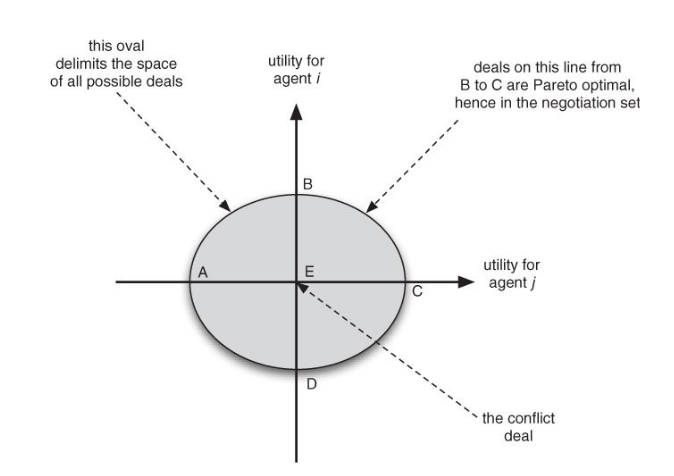
\includegraphics[width=.5\textwidth]{01/05}
\end{figure}
Here, the first, third and fourth quadrant includes the subset of deals that are not individual rational. (there is no point for an agent to accept a deal that produces negative utility).\\
Similarly, all deals strictly inside the ellipsis are not Pareto Optimal. Which brings as to the boundary of the negotiation set in the second quadrant.\\
Agent $i$ (ordinate axis) will start at its best possible deal (B), whereas agent $j$ (abscissa axis) will start at its best possible deal (C).\\
Both agent will then concede in one or more rounds until a point of mutual agreement on the boundary of the negotiation set is reached.

Task Oriented Domains assume that agents have symmetric cost functions (i.e. $c_i(T') = c_j(T')$) and that every agent is capable of handling tasks of all agents.\\
However, there exists other subtypes of Task oriented domains that consider different relations in the agents cost functions:
\begin{itemize}
\item \side{Subadditive TODs (STODs)} are TODs where:
\[c_i (T' \cup T'') \le c_i(T') + c_i(T'')\]
\item \side{Concave TODs (CTODs)} are subadditive TODs where:
\[c_i (T' \cup T'') - c_i(T') \ge c_i (T'' \cup T''') -  c_i(T'')\qquad \text{and }\qquad T' \subset T''\]
\item \side{Modular TODs (MTODs)} are concave TODs where:
\[c_i (T' \cup T'') \le c_i(T') + c_i(T'') - c_i (T'\cap T'')\]
\end{itemize} 

\begin{table}[!h]
\centering
\begin{NiceTabular}{ccccccccccccc}[hvlines]
&\Block{1-3}{TOD}&&&\Block{1-3}{STOD}&&&\Block{1-3}{CTOD}&&&\Block{1-3}{MTOD}&&\\
& Hid & Pha & Dec& Hid & Pha & Dec& Hid & Pha & Dec& Hid & Pha & Dec\\
Pure&L& L& L& L& L& L& L& L& L& L& & \\
Mixed&L& & L& L&  & L& L& & & L& & \\
All-or-nothing&& & & &  & L& & & & &  & \\
\end{NiceTabular}
\caption{The L states that lying is profitable and possible}
\end{table}


\subsection{Worth Oriented Domain}
 \phantom{c}\side{Worth Oriented domains} are domains where agents assign a worth to each potential state (of the environment), which captures its desirability for the agent.
\begin{itemize}
\item agent's goal is to bring about the state of the environment with highest value
\item We assume that the collection of agents has available set of joint plans (a joint plan is executed by several different agents). In other terms there is no possibility to complete a task alone.
\end{itemize}
Contrary to TOD, where tasks could have been achieved separately by both agents, in worth oriented domain the outcome can be achieved only by joint efforts (e.g. buying and selling are part of the worth oriented domain).
 
Formally, Worth oriented domains can be defined as a tuple
\[<E, Ag, J, c>\]
where:
\begin{itemize}
\item $E$: is the set of possible environment states/outcomes
\item $Ag$: is the set of possible agents
\item $J$: is the set of possible joint plans
\item $c(j,i)$: is the cost for agent $i$ of executing the plan $j$
\end{itemize}
Moreover, we will denote as $W(e,i)$ the value of worth of agent $i$ in state $e$.

Unlike, TODs, agents negotiating over Worth Oriented Domains are not negotiating about a single issue:
\begin{itemize}
\item They are negotiating over both the state that they wish to bring about (which has a different value for different agent)
\item They are negotiating over the means by which they will reach the state
\end{itemize}

Since this domain deals with multiple set of attributes, we are interested to find the Pareto Optimal solution. In order to do so we calculate the utility by:
\begin{itemize}
\item Weighting each attribute
\item Rating or ranking each attribute value
\item Using constraints on an attribute
\end{itemize}

The negotiation process will proceed to in rounds where each agent concedes, ultimately reaching an agreement or finding no agreement.

If the utility graphs representing the rating of each agent intersects at some point, then a point of acceptance is reached, otherwise the negotiation terminates in conflict.

\subsection{Monotonic Concession Protocol (MCP)}
The rules of this negotiation protocol are:
\begin{itemize}
\item Negotiation proceeds in a series of rounds
\item On the first round both agents simultaneously propose a deal from the negotiation set
\item An agreement is reached if the two agents propose deals $\delta_1$ and $\delta_2$, respectively, such that either:
\[utility_1(\delta_2) \ge utility_1(\delta_1)\qquad || \qquad utility_2(\delta_1)\ge utility_2(\delta_2)\]
\item If both agents offers match or exceed those of the other agent, then one of the proposals is selected at random
\item If only one proposal exceeds or matches the other's proposal, then this is the agreement deal
\item If no agreement is reached, then negotiation proceeds to another round of simultaneous proposals, where no agent is allowed to make a proposal that is less preferred by the other agent than the deal it proposed at the previous round
\item If neither agent makes a concession in some round, then negotiation terminates with the conflict deal
\end{itemize}

Using such protocol negotiation is guaranteed to end (with or without agreement) after a finite number of rounds, however the protocol does not guarantee that the agreement (or lack of it) will be reached quickly.
\subsection{The Zeuthen strategy}
\begin{enumerate}
\item What should an agent's first proposal be?
\item On any given round, who should concede?
\item If an agent concedes, then how much should it concede?
\end{enumerate}

With regard to the first question: an agent's first proposal should be its most preferred deal.

With respect to the second question: the idea of the \side{Zeuthen strategy} is to measure an agent's willingness to risk conflict (i.e. an agent is more willing to risk conflict if the difference in utility between its current proposal and the conflict deal is low).

Agent $i$'s willingness to risk conflict at round $t$ is:
\[risk^t_i = \cfrac{\text{utilty }i\text{ loses by conceding and accepting}j\text{`s offer} }{\text{utility }i\text{loses by not conceding and causing conflict}}\]
Until an agreement is reached, the value of risk is between 0 and 1 (the higher the value the higher the risk, which means that an agent has less to lose from conflict and as such it is more willing to risk conflict).\\
Formally:
\[risk^t_i =
\begin{dcases}
1 & \text{If }utility_i(\delta_i^t)=0\\
\cfrac{utility_i(\delta_i^t) - utility_i(\delta_j^t)}{utility_i(\delta_i^t)} &\text{otherwise}
\end{dcases}
\]
Hence, the zeuthen strategy proposes that the agent to concede on round $t$ of negotiation should be the one with the smaller value of risk.\\
Moreover, the agent in question should make the smallest concession necessary to change the balance of risk, so that on the next round, the other agent will concede.

Lastly, in the case of equal risk, a coin flip will decide which agent should concede, otherwise we are in the same situation of the prisoner's dilemma.

We notice that the Zeuthen strategy and the protocol itself:
\begin{itemize}
\item Does not guarantee success, but it does guarantee termination
\item It does not guarantee to maximize social welfare
\item If agreement is reached, then this agreement will be Pareto Optimal
\item It is individual rational
\item It is in Nash equilibrium (if an agent is using the Zeuthen strategy the other can do no better than using the same strategy)
\end{itemize}

\subsection{Deception}

There are three obvious ways in which an agent can be deceitful in Task oriented domain:
\begin{itemize}
\item \side{Phantom tasks}\\
An agent can pretend to have been allocated a task that it has not been allocated.

An obvious respoinse to these is to ensure that the tasks an agent has been assigned to carry out are verifiable by all negotiation participants.
\item \side{Decoy tasks}\\
An agent can prodice an artificial task when asked for it.

Detection of decoy tasks is esssentially impossible, mmaking it hard to be sure that deception will occur in such domains.
\item \side{Hidden tasks}\\
An agent may benefit from deception by hiding tasks that it has to perform
\end{itemize}
Using mixed deals or all-or-nothing deals helps to get rid of deceptions:
\begin{itemize}
\item probability is assigned to each Agent task
\item all or nothing deal is applied
\item weighted coin (with probabilities) is used
\item In case of phantom and decoy tasks, the deceiving agent can have a bigger probability to be assigned all the tasks, hence it has no advantage in lying
\item However, it is possible that decoy tasks do not increase probability to be allocated all the tasks in some topology
\end{itemize}

This cas aspect can be further proven with an example:
\begin{figure}[!h]
\centering
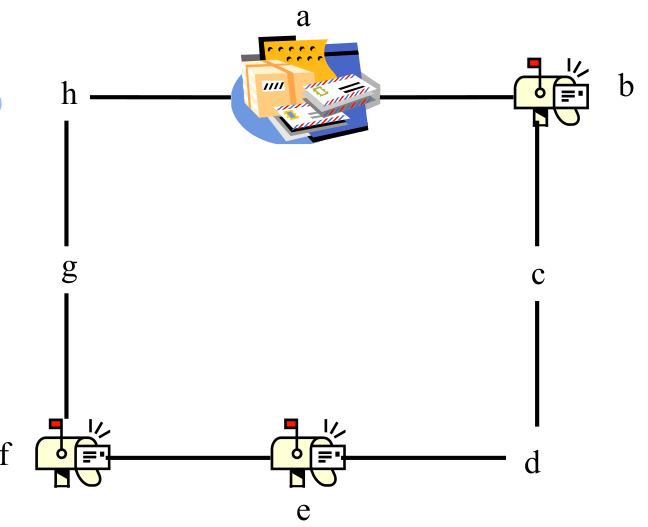
\includegraphics[width=.5\textwidth]{01/06}
\end{figure}
Two postmen need, for some obscure reason to redistribute their letters:
\begin{itemize}
\item Agent $i$, has to deliver letter $b$ and $f$
\item Agent $j$, has to deliver a letter to $e$
\end{itemize}
Agent $i$ decides to deceive the other agent and hide the letter $b$.

However, if the two agents use a weighted coin and a all-or-nothing deal to reallocate their task, deceiving becomes disadvantegeous from a probabilistic standpoint. 
In order to understand why let us consider a simple model of the probability based on the edges that an agent has to traverse:
\begin{itemize}
\item Agent $i$ (the deceiving one) have an expected cost that has the following form:
\[expected\,cost = \sfrac{3}{8}\cdot 8 + \sfrac{5}{8}\cdot2 = 4.25\]
The expected cost components are derived in the followin way:
\begin{itemize}
\item Compute the probabilities based on the claimed letters to deliver.

Agent $i$ claims to have only the letter $f$ to deliver which is at a distance of 3 edges from the post office. Since there are a total of 8 edges, the associated probability is $3/8$. As a result, the probability of winning the coin flip is $1-\sfrac{3}{8} = \sfrac{5}{8}$
\item Compute the cost of delivering the letter (which is the number of edges forward and back to traverse).

In the case of agent $i$, losing the coin flip will imply that he has to deliver all the letters (all-or-nothing deals). The shortest path to do so implies traversing all of the 8 edges of the graph, hence the associated cost is 8.

On the contrary if agent $i$ wins the weighted coin flip, it has still to deliver the hidden letter $b$ which would require him to traverse 1 edge forward and back, resulting in a total cost of 2.
 
\end{itemize}
\item From the expected cost result we can then compute the utility that agent $i$ obtained by hiding the letter: this value is compute as the difference of traversing the whole graph with the expected cost:
\[utility = 8-4.25 = 3.75\]
\item We can notice that if agent $i$ would have not hidden the letter, it would have gotten a coin flip probability of $\sfrac{4}{8}= 0.5$ since the sum of the edges that he would have had to traverse is 3 for the letter $f$ and 1 for the letter $b$.
Whereas the cost of winning the coin flip would have been 0 (no letters to deliver), and the cost of losing the coin flip is 8 (the postman has to deliver all the letters which means that it has to traverse the whole graph).

Hence the expected cost of not lying would have been:
\[expected\,cost = 0.5 \cdot 8 + 0.5\cdot 0 = 4\]
and as a result the utility would have been:
\[utility = 8-4 = 4\]
which is higher than the utility of hiding the letter $b$
\end{itemize}

\section{Contract Net Protocol (CNP)}
Cooperating experts metaphor:
\begin{itemize}
\item work independently
\item exchange results
\item ask help when enable to solve individually
\end{itemize}

The assumptions that CNP makes is that
\begin{itemize}
\item If the problem is too large then partition it and find other experts who can solve the task
\item If the problem is outside of expertise then also findanother expert
\item If expert is known then contact them directly, otherwise describe the task to the entire group of agents
\item If somebody from the group agree then the agent will notifies it
\item If more then one agree then choose one
\end{itemize}

The basic premise of the CNP is that, if an agent cannot solve an assigned problem using local resources/expertise, it will decompose the problem into subproblems and try to find other willing agents with the necessary resource/expertise to solve these subproblems

In this sense, each agent can take one of two roles: \side{manager} or \side{contractor}.

The overall contracting mechanism goes as follows:
\begin{enumerate}
\item contract announcement by the manager agent
\item submission of bids by contracting agents in response to the announcement
\item evaluation of submitted bids by the manager
\item awarding a subproblem contract to the contractor with the most appropriate bids
\end{enumerate}
Contrary to auctions, there is no limitations in respecting the bid that agent have made: this means that even though an agent wins a bid and accept a given task it is not forced to take it.

Formally, Let us consider:
\begin{itemize}
\item $\tau_i^t$ the set of tasks allocated to the agent $i$ at time $t$
\item $e_i$ the resources available to $i$
\item $\tau(ts)$ the announce task
\end{itemize}

The \side{marginal cost} proposed by Sandholm, takes the form:
\[\mu_i(\tau(ts)|\tau_i^t) = c_i(\tau(ts) \cup \tau_i^t) - c_i(\tau_i^t)\]

Hence the decision to bid happens if and only if 
\[\mu(\tau(ts)|\tau_i^t) < (e(ts) + e_i)\]
where $e(ts)$ is reward for doing the new task

The problems with CNP are:
\begin{enumerate}
\item it does not detect conflicts
\item it assumes benevolent and non-antagonistic agents
\item it is still rather communication intensive
\end{enumerate}
    \chapter{Agent Communication}
\label{ch:AgentCommunication}

\minitoc

Communication has been a topic of extensive study in the field of computer science. Particularly, the problem of \side{synchronization} of multiple processes was of key interest in the 1970s and 1980s.

This is of importance since processes have fundamentally the same behaviour of agents. In fact, the object oriented paradigm would require \side{communication via method invocation} to allow an object to message another and change its internal state (this is not allowed in an agent-oriented setting).

Let us consider, for example, two agents $i$ and $j$, where $i$ has the capability to perform an action $\alpha$ (similar to a method).\\
In an agent-oriented world, contrary to object-oriented, there is no such thing as method invocation. This is because both $i$ is an \side{autonomous agent}, and as such it has control over both its state and behaviour.\\
Hence, it cannot be taken for granted that agent $i$ will execute action $\alpha$ just because another agent $j$ wants it to: performing the action may not be in the best interests of agent $i$.

In general, agents can neither force other agents to perform some action, nor write data onto the internal state of other agents, but this does not mean that they cannot communicate.\\
What agents can do is perform \side{communicative actions} in an attempt to \side{influence} other agents.

\section{Approaches to software interoperation}
We intiially consider \side{software interoperation}, i.e. the exchange of information and services with other programs, thereby solving problems that cannot be solved alone.\\
This is fundamentally different from communication (interaction between humans).

The main problem related with software interoperation is \side{heterogeneity}, in the sense that two or more software in need to interoperate might be written by different people, at different times and in different languages.

Hence, in order for them to communicate successfully it should be provided:
\begin{itemize}
\item a standard communication language
\item common libraries
\item run time support
\end{itemize}
And particularly, we would like to answer the following questions:
\begin{itemize}
\item What is an appropriate agent communication language?
\item How do we build agents capable of communicating in this language?
\item What communication architectures are conductive to cooperation?
\end{itemize}

\subsection{Components of a system for effective interaction and interoperability}
The basic components of a system to achieve effective software interaction adn interoperability are:
\begin{itemize}
\item a common language
\item a common understanding of the knowledge exchanged (common understanding of the components of the language as well as their meaning)
\item the ability to exchange whatever is included in the previous items.
\end{itemize}

The reason why we cannot use natural language as a common language for agent communication is that it is not easy to develop system that understands it completely. 
Moreover, the use of other communication protocols such as xml or json it is not ideal since agents have conversations (as opposed to exchange of single messages).

In addition to this the communication behaviour should allow to express agents strategies, intentions, roles, ..., i.e. concepts that are high level than can be expressed in low level languages.

\subsection{Three Important Aspects}
There are three important aspects in communication:
\begin{enumerate}
\item \side{Syntax}: how the symbols of communication are structured.

It includes the grammatical rules, how we write and so on.
\item \side{Semantics}: what the symbols denote
\item \side{Pragmatics}: How the symbols are interpreted, what is the context of the communication. The same sentence can be interpreted in different ways.
\end{enumerate} 

The combination of semantics and pragmatics is the \side{meaning} of the communication.

From the above, we deduce that an agent communication language (ACL) should be:
\begin{enumerate}
\item Syntactic: should allow syntactic translation between the agents
\item Meaning: should allow meaning content preservation among applications.
\item Communication: should be able to communicate complex attributes about their information and knowledge.
\end{enumerate}
Hence what distinguish ACLs from other languages is:
\begin{itemize}
\item Semantic complexity
\item ACLs can handle propositions, rules and actions instead of simple objects with no semantics associated with them. Hence ACL does not deal with a simple exchange of data, but instead with the exchange of information that has a meaning.
\item An ACL message describes a desired state in a declarative language, rather than a procedure or a method. 
\end{itemize}


\section{Speech Acts}
\phantom{c}\side{Speech acts theory} treats communication as action. It is predicated on the assumption that speech actions are performed by agents just like other actions, in the furtherance of their intentions.

As such, speech act theories attempt to account for how language is used by people every day to achieve their goals and intentions. 

\subsection{Austin}
The theory of speech acts is generally recognized to have begun with the work of the philosopher John Austin. He noted that a certain class of natural language utterances, referred to as \side{speech acts}, had the characteristics of actions, in the sense that they change the state of the world in a way analogous to physical actions.

Austin identified a number of \side{performative verbs}, which correspond to various different types of speech acts (e.g. request, inform, promise).\\
In addition, Austin distinguished three different aspects of speech acts:
\begin{enumerate}
\item \side{locutionary act}: act of making an utterance
\item \side{illocutionary act}: action performed in saying something
\item \side{perlocution}: effect of the act
\end{enumerate}
Austin referred to the conditions required for the successful completion of performatives as \side{felicity conditions}, that are as follows:
\begin{itemize}
\item There must be an accepted conventional procedure for the performative, and the circumstances and persons must be as specified in the procedure
\item The procedure must be executed correctly and completely
\item The act must be sincere and any uptake required must be completed insofar as is possible
\end{itemize}

We are particularly interested in the illocutionary act.\\ Formally, an illocutionary act $F(P)$ si composed from:
\begin{itemize}
\item \side{propositional content} $P$: what is the utterance or message exchanged
\item \side{context}: context of the message
\item \side{illocutionary force} $F$: what is the intention of the message
\end{itemize}


The illocutionary force divides speech acts into categories described by :
\begin{itemize}
\item \side{Illocutionary point} 
\item \side{direction of fit}, is the coveyed message describing the world or changing the world
\item \side{sincerity conditions}
 \end{itemize}
\subsection{Searle}

Searle extended the work of Austin in his 1969 book \emph{Speech Acts}.
%For our use we are going to consider only the illocutionary act.\\
Searle identified several properties that must hold for a speech act prefromed between a \side{HEARER} and a \side{SPEAKER} to succeed.
\begin{enumerate}
\item \side{Normal I/O Conditions}: the HEARER is able to hear the performative of the speaker and the act was performed in normal circumstances (not in a film or a play).
\item \side{Preparatory conditions}: state what must be true of the world in order that SPEAKER correctly choose the speech act (in a request to perform ACTION, the HEARER must be able to perform such ACTION and the SPEAKER must believe the HEARER is able to perform such ACTION)
\item \side{Sincerity conditions}:these conditions distinguish sincere performatives of the request; an insincere performance of the act might occur if SPEAKER did not really want ACTION to be performed.
\end{enumerate}

Searle also attempted a systematic classification of possible types of speech acts identifying the followin five key classes:
\begin{itemize}
\item \side{Representatives} (inform): a representative act commits the speaker to the truth of an expressed proposition
\item \side{Directives} (request): a directive is an attempt on the part of the speaker to get the hearer to do something
\item \side{Commissives} (promise): Commit the speaker to a course of action
\item \side{Expressives} (thanking): Express some psychological state such as gratitude
\item \side{Declarations} (declaring war): Effect some changes in an institutional state of affairs
\end{itemize}
Later some additional speech acts were introduces: \side{Permissives} and \side{Prohibitives}

%\begin{table}[!h]
%\centering
%\begin{NiceTabular}{|c|c|c|c|}
%\hline
%\textbf{Illocutionary act}& \textbf{Illocutionary point}&\textbf{Direction of fit} & \textbf{Sincerity condition}\\
%\hline
%\Block{2-1}{Assertives/\\Representatives }&\Block{2-1}{Commits speaker to \\truth of utterance}&\Block{2-1}{world $\rightarrow$ word\\(describe world)}&\Block{2-1}{Speaker believes \\utterance}\\
%&  &  & \\
%\hline
%\Block{2-1}{Directives } & \Block{2-1}{Speaker tries to make \\hearer do something }& \Block{2-1}{word $\rightarrow$ world \\(change world)}& \Block{2-1}{Speaker wants Hearer to \\establish the truth of utterance}\\
%&  &  & \\
%\hline
%\Block{3-1}{Commisives}&\Block{3-1}{Commits Speaker to \\future action}&\Block{3-1}{word $\rightarrow$ world \\(change world)}& \Block{3-1}{Speaker intends to act \\such that the truth of the \\utterance is established}\\
%&&&\\
%&&&\\
%\hline
%\Block{2-1}{Expressives}&\Block{2-1}{Express psychological state}&\Block{2-1}{None}&\Block{2-1}{Several possibilities}\\
%&&&\\
%\hline
%\Block{2-1}{Declaratives}&\Block{2-1}{Establish correspondence between \\utterance and world}&\Block{2-1}{world $\rightarrow$ word \\word $\rightarrow$ world}&\Block{2-1}{None}\\
%&&&\\
%\hline
%\end{NiceTabular}
%\end{table}

\subsection{Plan-based theory}
In order for an AI to make a plan about how to achieve goals from the interaction with humans or other autonomous agents, such plans must include speech actions.  Formally the aim of the application of such mechanism is to develop a theory of speech acts\\
\say{... by modelling them in a planning system as operators defined... in terms of speakers' and hearers' beliefs and goals. Thus speech acts are treated in the same way as physical actions}.

Cohen and Perrault came up with a formalism called the \side{STRIPS} notation, in which the properties of an action are characterized via \side{precondition}s and \side{postcondition}s.\\
Cohen and Perrault also demonstrated how the preconditions and postconditions of speech acts could be represented in a multimodal logic containing operators for describing the beliefs, abilities and wants of the participants in the speech act.

In short, in order for a speech act to be successful the preconditions must be fullfilled; however the fulfillment of the preconditions are not enough in itself to guarantee that the desired action will actually be performed. This is because some speech act such as request or inform only models the illocutionary force of the act, not the perlocutionary force.

For this reason, Cohen and Perrault introduced some mediating act: Convince and CauseToWant; which respectively will make the hearer believe an inform act and believe that the speaker of a request act wants the hearer to do an action.
\begin{table}[!h]
\centering
\begin{NiceTabular}{|lll|}
\hline
\Block{1-2}{$Request(S, H, \alpha)$}&&\\
\hline
Precondition& Cando.pr&$(S\,\,BELIEVE\,\,(H\,\,CANDO\,\,\alpha))\,\land$\\
&&$(S\,\,BELIEVE\,\,(H \,\,BELIEVE\,\,(H\,\,CANDO\,\,\alpha)))$\\
& Want.pr &$(S\,\,BELIEVE\,\,(S\,\,WANT\,\,requestInstance))$\\
Effect&&$(H\,\,BELIEVE\,\,(S\,\,BELIEVE\,\,(S\,\,WANT\,\,\alpha))$\\
\hline
\Block{1-2}{$CauseToWant(A_1, A_2, \alpha)$}&&\\
\hline
Precondition& Cando.pr&$(A_1\,\,BELIEVE\,\,(A_2 \,\,BELIEVE\,\,(A_2\,\,WANT\,\,\alpha)))$\\
& Want.pr &$\times$\\
Effect&&$(A_1\,\,BELIEVE\,\,(A_1\,\,WANT\,\,\alpha))$\\
\hline
\Block{1-2}{$Inform(S, H, \phi)$}&&\\
\hline
Precondition& Cando.pr&$(S\,\,BELIEVE\,\,\phi)$\\
& Want.pr &$(S\,\,BELIEVE\,\,(S\,\,WANT\,\,informInstance))$\\
Effect&&$(H\,\,BELIEVE\,\,(S\,\,BELIEVE\,\,\phi))$\\
\hline
\Block{1-2}{$Convince(A_1, A_2, \phi)$}&&\\
\hline
Precondition& Cando.pr&$(A_1\,\,BELIEVE\,\,(A_2\,\,BELIEVE\,\,\phi))$\\
& Want.pr &$\times$\\
Effect&&$(A_1\,\,BELIEVE\,\,\phi)$\\
\hline
\end{NiceTabular}
\end{table}

\subsection{Speech acts as rational actions}
While the plan-based theory of speech acts was a major step forward, it was recognized that a theory of speech acts should be rooted in a more general theory of rational action.\\
This led Cohen and Levesque to develop a theory in which speech acts were modelled as actinos performed by rational agents in the furtherance of their intentions.\\
The foundation upon which they built this model of rational action was their theory of intention.

\section{Agent Communication Languages (ACL)}
In the ACL we strive to communicate or exchange the meaning explicitly by saying what is the intention in the language. This is in contract with the human language in which the meaning is hidden by the words used, the intonation, the tone (it is not always explictly said).

There are some fundamental components of the language that may help to achieve a language that explicitly communicate meaning:
\begin{itemize}
\item An illocutionary force represented by a performative verb. (e.g. request, inform)
\item Propositional content, what the agent said.
\end{itemize}
This makes it so that different propositional content can be interpreted in different ways by the hearer based on the associated illocutionary force.

The semantic of speech acts can be represented via plan-based theory, which treats speech acts as physical actions. Thus, each action is characterised by preconditions (conditions that must be fulfilled for successful communication) and postconditions (effect).

\subsection{KSE}
Speech act theories have directly informed and influenced a number of languages that have been developed specifically for agent communication.\\
In the early 1990s, the US-based DARPA-funded Knowledge Sharing Effort (KSE) was formed.

The KSE generated threemain deliverables:
\begin{itemize}
\item The \side{Knowledge Interchange Format (KIF)}.\\
This language was explicitly intended to allow the representation of knowledge about some particular domain of discourse (aka the content of the message).
\item The \side{Ontolingua}\\
Ontology representation.
\item The \side{Knowledge Query and Manipulation Language (KQML)}. \\
This language defines an envelope format for messages, but is not concerned with the content part of the messages.
In short, it defines the language for both message formatting and message handling protocols
\end{itemize}
The Basic assumption that KSE makes is that 
\say{Software agents are applications for which ability to communicate with other applications and share knoledge is of primary importance.}
In the KSE case, the basic components of an ACL are represented as follows:
\begin{itemize}
\item Communication, through a interaction protocol, communication language and a transport protocol
\item Representation, through knowledge bases and ontologies (way of representing organization of knowledge, how concept are organized and what is their meaning, set of symbols with their associated meaning)
\item Supporting components, through planning activities, modeling other agents and environments, meta-knowledge (how we can reason about what we know) and reasoning
\end{itemize}
\subsubsection{KIF}
The Knowledge Interchange Format (KIF) was intended to:
\begin{itemize}
\item  create a language for development of intelligent applications. 
\item create a common interchange format that allows to translate from any language to it and vice versa.
\item  express the contents of a message but not the message itself.
\end{itemize}
KIF was not intended to:
\begin{itemize}
\item to model the interaction with human user
\item to be internal representation for knowledge within computer programs.
\end{itemize}

The interchange format that KIF uses is best described with an example.\\
Let us assume we have two languages ($L_1$ and $L_2$). In this scenario we need to develop two translations in order to have communication between the two agents.\\
If we have three languages, the number of translations is 6\\
If we have four languages, the number of translations is 12\\

We can notice that as the number of languages increases the number of translations necessary increases drastically, for this reason an intermediate language from and to other languages are translated was proposed under the name of KIF.
It means the for each language we need to develop only two translations. \\

KIF is a prefix version of first order predicate calculus.
\begin{itemize}
\item The prefix version tells that first we place the operation then the operands 
\item KIF has a declarative semantics\\
you do not need to say how it will be executed in the interpreter but instead you can present your statement in some arbitrary order and then an inference mechanism will find a way in which it can be operated
\item KIF is logically comprehensive.\\
allows to represent all necessary logic constraints
\item KIF provides for representatino of knowledge about representation of knowledge (meta-level)
\end{itemize}
Additional features are:
\begin{itemize}
\item Translatability, easy to represent
\item Readability, easy to read
\item Usability as a representation language 
\end{itemize}

Using KIF, it is possible to express:
\begin{itemize}
\item Properties of things in a domain
\item Relationships between things in a domain
\item General properties of a domain
\end{itemize}

In order to do so, KIF has introduced:
\begin{itemize}
\item Variables: ordinary variable represented with a $?$ prefix and list variables represented with a $@$ prefix
\item Operators
\begin{itemize}
\item term operators: e.g. listof, if, ...
\item sentence operators: e.g. not, and, $/=$, ...
\item rule operators: e.g. $=>>$, ...
\item definition operators: e.g. defobject, deffunction,...
\end{itemize}
\item Constants
\begin{itemize}
\item object constants
\item function constants
\item relational constants
\item logical constants
\end{itemize}
\item Expressions/Sentences: word or a finite sequence of words
\end{itemize}
\subsubsection{Ontologies}
An ontology is a formal explicity specification of a shared conceptualization.

An ontology is a description of the concepts and relationships that can exist for an agent or a community of agents. \\
The reason why we need ontology is that agents need to have the same understanding of concepts that we use.

An example is the world VISA, which can be both a entering permit or a credit card. We therefore can specify an ontology for traveling and one for finance and distinguish between the two.

Hence, ontology is used to agree on a terminology to describe a domain, and by referencing this ontology we communicate the meaning of the communication.\\
Ontolingua is one of the first ontologies developed that was used to give notion or meaning of words that we use in KIF.


\subsubsection{KQML}
KQML is a message-based language for agent communication. Thus KQML defines a common format for messages.

Each KQML object has a \side{performative} and a number of \side{parameters}.

An example of a KQML object is 

\begin{lstlisting}[language=C++]
{$performative$
	:content $content$
	:receiver $receiver$
	:language $language$
	:ontology $ontology$
}
\end{lstlisting}

KQML defines a set of standard performatives to choose from of which different parameters are required. 
In table \ref{tbl:KQMLper} the list of 41 performatives are proposed with their meaning and in table \ref{tbl:KQMLparams} the list of the main parameters of KQML messages are summarized.

\begin{table}[!h]
\centering
\begin{NiceTabular}{ll}[hvlines]
\textbf{Parameter} & \textbf{Meaning}\\
\texttt{:content}& content of the message\\
\texttt{:force}&whether the sender will ever deny the content of the message\\
\texttt{:reply-with}&whether the sender expects a reply, and, if so, an identifier for the reply \\
\texttt{:in-reply-to}& reference to the \texttt{:reply-with} parameter\\
\texttt{:sender}&sender of the message\\
\texttt{:receiver}&intended recipient of the message
\end{NiceTabular}
\caption{Parameters for KQML messages}
\label{tbl:KQMLparams}
\end{table}

\begin{table}[!h]
\centering
\begin{NiceTabular}{ll}[hvlines]
\textbf{Performative} & \textbf{Meaning}\\
\texttt{achieve}&S wants R to make something true of their environment\\
\texttt{advertise}&S claims to be suited to processing a performative\\
\texttt{ask-about}&S wants all relevant sentences in R’s VKB\\
\texttt{ask-all}&S wants all of R’s answers to a question C\\
\texttt{ask-if}&S wants to know whether the answer to C is in R’s VKB\\
\texttt{ask-one}&S wants one of R’s answers to question C\\
\texttt{break}&S wants R to break an established pipe\\
\texttt{broadcast}&S wants R to send a performative over all connections\\
\texttt{broker-all}&S wants R to collect all responses to a performative\\
\texttt{broker-one}&S wants R to get help in responding to a performative\\
\texttt{deny}&the embedded performative does not apply to S (any more)\\
\texttt{delete-all}&S wants R to remove all sentences matching C from its VKB\\
\texttt{delete-one}&S wants R to remove one sentence matching C from its VKB\\
\texttt{discard}&S will not want R’s remaining responses to a query\\
\texttt{eos}&end of a stream response to an earlier query\\
\texttt{error}&S considers R’s earlier message to be malformed\\
\texttt{evaluate}&S wants R to evaluate (simplify)C\\
\texttt{forward}&S wants R to forward a message to another agent\\
\texttt{generator}&same as \texttt{standby} of a \texttt{stream-all}\\
\texttt{insert}&S asks R to add content to its VKB\\
\texttt{monitor}&S wants updates to R’s response to a stream-all\\
\texttt{next}&S wants R’s next response to a previously streamed performative\\
\texttt{pipe}&S wants R to route all further performatives to another agent\\
\texttt{ready}&S is ready to respond to R’s previously mentioned performative\\
\texttt{recommend-all}&S wants all names of agents who can respond to C\\
\texttt{recommend-one}&S wants the name of an agent who can respond to a C\\
\texttt{recruit-all}&S wants R to get all suitable agents to respond to C\\
\texttt{recruit-one}&S wants R to get one suitable agent to respond to C\\
\texttt{register}&S can deliver performatives to some named agent\\
\texttt{reply}&communicates an expected reply\\
\texttt{rest}&S wants R’s remaining responses to a previously named performative\\
\texttt{sorry}&S cannot provide a more informative reply\\
\texttt{standby}&S wants R to be ready to respond to a performative\\
\texttt{stream-about}&multiple response version of ask-about\\
\texttt{stream-all}&multiple response version of ask-all\\
\texttt{subscribe}&S wants updates to R’s response to a performative\\
\texttt{tell}&S claims to R that C is in S’s VKB\\
\texttt{transport-address}&S associates symbolic name with transport address\\
\texttt{unregister}&the deny of a register\\
\texttt{untell}&S claims to R that C is not in S’s VKB
\end{NiceTabular}
\caption{Performatives for KQML messages}
\label{tbl:KQMLper}
\end{table}

To more fully understand these performatives, it is necessary to understand the notion of a \side{virtual knowledge base (VKB)} as it was used in KQML. The idea was that agents using KQML to communicate may be implemented using different programming languages and paradigms and any information that agents have may be internally represented in many different ways. However, for the purpose of communication, it makes sense for agents to treat other agents as if they had some internal representation of knowledge.  \\
This attributed knoledge is known as the virtual knowledge base.\\

Despite the initial success, KQML was subsequently criticized on a number of grounds:
\begin{itemize}
\item The basic KQML performative set was rather fluid. It was never tightly constrained, and so different implementatinos of KQML were developed that could not, in fact, interoperate
\item Transport mechanisms for KQML messages were never precisely defined
\item The semantics of KQML was never rigorously defined. this is because the meaning of KQML performatives was only defined using informal, English language descriptions, open to different interpretations (it was impossible to tell whether to agents were using KQML language properly)
\item The lenguage was missing an entire class of performatives, such as commissives (which are a requirement for agent coordination)
\item The performative set for KQML was overly large and, it could be argued, rather ad hoc.
\end{itemize}

In an environment it is good to have language, but we need some supporting elements which are \side{Facilitators}. Facilitators are used to route the message in case an agent does not know exactly the address of the receiver.\\
In this sense, facilitators help to make communication protocol transparent.

We can think of facilitators as a special class of agents that perform useful communication services such as:
\begin{itemize}
\item Maintain registry of service names
\item Forward messages to named services
\item Routing messages based on content (not the content of the message but rather ontology and language)
\item Provide matchmaking betweeen information providers and requesters
\item Provide mediation and translation services
\item  ....
\end{itemize}

In particular KQML defines a standard protocol to be implemented by facilitator:
\begin{itemize}
\item \side{Point-to-Point protocol} \\
If A is aware about B then it is appropriate to send query about X to B.\\
In other terms if agent A knows exactly agent B then it is allowed to reach and communicate with it directly
\item \side{Subscribe performative}\\
Request that Facilitator F helps find the truth of X. If B subsequently informs F that it believes X to be true, then F can in turn inform A
\item \side{broker performative}\\
A asks Facilitator to find another agent (not F) which can process a given performative. (agent A does not ask value of X, but rather someone who can process X)
\item \side{recruit performative}\\
Asks Facilitator to find an appropriate agent to which an embedded performative can be forwarded. A reply is returned directly to the original agent
\item \side{recommend performative}\\
Asks Facilitator to respond with the name of another agent which is appropriate for sending a particular performative 
\end{itemize}

Another element of interest of KQML is its internal structure.\\
The communication architecture is built around three main elements:
\begin{enumerate}
\item facilitators.\\
Facilitators are agents with own KQML routers, they are no different (in implementation) from other agents.
The only things that makes them different from regular agents is that they have some predefined functionality about a particular facilitating communication.\\
Tipically one facilitator for each local group of agents.
\item routers.\\
Content independent message routers.\\
Each KQML agent is associated with its own separate router process.\\
router handles all KQML messages going to and from the associated agent.\\
can try to find Internet address for service and deliver message to it.
\item Library of interfaces (KRIL)\\
\side{Router Interface Library (KRIL)}\\
It is a programming interface between router and agent.\\
It is embedded into application\\
The main role of KRIL to make access to the router as simple as possible for the programmer\\
API are developed for different languages and then these API can be used directly in agent in order to make communication, tipically with primitives to send message and it defines some point of  listening in which messages from other agents will be accomodated and processed.
\end{enumerate}
In general, KQML allows us to implement the system via some independent routing mechanism without involving a particular agent in the knowledge of such mechanism.

It says that we can provide routers that can route network between different engines  and in order to communicate with routers we provide some predefined interface that one can embed in you agent.
\subsection{FIPA ACL}
In 1995, the \side{Foundation for Intelligent Physical Agents (FIPA)} began its work on developing standard for agent systems. The centerpiece of this initiative was the development of an agent communication language (ACL).

The FIPA ACL is superficially similar to KQML, since:
\begin{itemize}
\item It defines an outer language for messages
\item It defines 20 performatives for defining the intended interpretation of messages,
\item it does not mandate any specific language for message content
\end{itemize}
In additino the concrete syntax for FIPA ACL messages closely resembles that of KQML

\begin{lstlisting}[language=C++]
{$performative$
	:sender $sender$
	:receiver $receiver$
	:content $content$
	:language $language$
	:ontology $ontology$
}
\end{lstlisting}
Hence the structure of messages is the same and the message attribute fields are also very similar, however the most important difference between the two languages is the collection of performatives they provide.

\begin{table}[!h]
\centering
\begin{NiceTabular}{lccccc}
\hline
& \Block{2-1}{Passing\\Information}&\Block{2-1}{Requesting Information}&&\Block{2-1}{Performing\\actions}&\Block{2-1}{Error\\handling}\\
Performative&&&Negotiation&&\\
\hline
\texttt{accept-proposal}&&&$\times$&&\\
\texttt{agree}&&&&$\times$&\\
\texttt{cancel}&&$\times$&&$\times$&\\
\texttt{cfp}&&&$\times$&&\\
\texttt{confirm}&$\times$&&&&\\
\texttt{disconfirm}&$\times$&&&&\\
\texttt{failure}&&&&&$\times$\\
\texttt{inform}&$\times$&&&&\\
\texttt{inform-if}&$\times$&&&&\\
\texttt{inform-ref}&$\times$&&&&\\
\texttt{not-understood}&&&&&$\times$\\
\texttt{propagate}&&&&$\times$&\\
\texttt{propose}&&$\times$&&&\\
\texttt{proxy}&&&&$\times$&\\
\texttt{query-if}&&$\times$&&&\\
\texttt{query-ref}&&$\times$&&&\\
\texttt{refuse}&&&&$\times$&\\
\texttt{reject-proposal}&&&$\times$&&\\
\texttt{request}&&&&$\times$&\\
\texttt{request-when}&&&&$\times$&\\
\texttt{request-whenever}&&&&$\times$&\\
\texttt{subscribe}&&$\times$&&&\\
\hline
\end{NiceTabular}
\end{table}

FIPA provides some standardization of agent interaction protocols.\\
Ongoing conversations between agents fall into typical patterns. In such cases, certain message sequences are expected and at any point in the conversation other messages are expected to follow.\\
These typical patterns of message exchange are called protocols.

FIPA does not allow a protcol to be up to interpretation, for this reason they provide some  standardized version of each multiagent interactions  such as actions or voting or others and specify exactly how these interactions should be carried on.
	
    \chapter{Agent Coordination}
\minitoc

Coordination is \say{the process by which an agent reasons about its local actions and the anticipated actions of other to try and esure that the community acts in a coherent manner.}

\section{General models}
In some sense coordination is the normal way of operating MASs, in which agents can plan their activities based on what they perceive around them. However, during this process agents can incur into some conflicts that are solved via Negotiation.\\
As a consequence, Coordination in the normal behaviour of the agents, whereas Negotiation is exception handling.

\subsection{Motivation}
The reasons why we need cooperation between agents is for:
\begin{itemize}
\item Preventing anarchy or chaos.\\
If agents do not coordinate their behaviour than cause will arise in the system quite quickly
\item Meeting global contraints.\\
In particular, if a budget is given to some agents when reasoning about a project, there is a budget constraint that needs to be satisfied.
\item Distributed expertise, resources or information.\\
Because in many cases we have some sofisticated expertise by different actors and we would like them to work them together.
\item Dependencies between agents' actions.
\item Efficiency\\
The exchange of information with other agents may increase the efficiency of the solution.
\end{itemize}

\subsection{Coordination properties and mechanisms}
Each coordination mechanism needs to ensure:
\begin{itemize}
\item \side{Coverage}. \\
Given a common area of operation, all the portions of the problem are included into the activity of at least one agent.
\item \side{Connectivity}.\\
Agents interact in a way that allow their activity to be integrated into the final overall solution.
\item \side{Rationality}.\\
Team members act in purpose in a consistent way.
\item \side{Capability}.\\
All objectives must be achievable within available computational and resource limitations.
\end{itemize}

Moreover the activities that the mechanism needs, while operating, to perform is to:
\begin{itemize}
\item supply timely information to needly agents
\item ensure synchronization
\item avoid redundant problem solving
\end{itemize}
 
The question ramains on how a designer achieve coherent behaviour of the system and in particular of each agents. There are three approaches to achieve coherent behaviour:
\begin{itemize}
\item \side{complete knowledge}.\\
Each agent knows completely what other agents do and based on this knowledge the agent will reason about its own activity
\item \side{centralized control}.\\
A designated agent will decide about the allocation of tasks and how these tasks can be used and synchronized
\item \side{distributed control}.\\
No agent has overview of tasks and agents reach coordination/coherent behaviour via negotiation or taking into consideration the activity of nearby agents
\end{itemize}

Fundamental coordination processes:
\begin{itemize}
\item \side{Mutual adjustment}.\\
Agents will adjust their behaviour based on the behaviour of other agents.
\item \side{Direct supervision}.\\
An agent will tell nearby agents to change their behaviour.
\item \side{Standardization}.\\
Standardization of what can be done and what should be avoided, and based on that agents will try to adjust their own behaviour based on some rules.
\end{itemize}

\subsection{Coordiantion problem}
In order to tackle the coordination problem there are several steps that we must take:
\begin{itemize}
\item analysis of a perspective for coordination
\begin{itemize}
\item external observation.\\
Based on the behaviour of others each agent adjust its behaviour. However it may be not enough because:
\begin{itemize}
\item behaviour can be coordinated but incoherent.\\
An agent might try to reason about the course of actions but it does not interpret other agents' actions correctly.
\item behaviour can be coherent but non-coordinated.
\end{itemize}
\item examining internal goals and motivations is necessary.\\
Which implies that having a model of behaviour of other surrounding agents can help establish coordination in MASs
\end{itemize}
\item applying appropriate coordination model.\\
An agent will need to have a general model of coordination that fits all the cases that might occur which will be a purely mathematical approach. 
\end{itemize}

\subsubsection{Control decisions and search}
View to coordination as a matter of effective control of distributed search.\\
Almost every problem can be interpreted as a search problem, and it is a process of looking at a sequence of actions that react to a goal or look at some subgoal to reach a  solvable goal.

In other terms, in any case an agent has complete knowledge of the current  situation, has access to sequence of possible actions and it can try to combine every possible actions to reach a goal.

Thus, control in this sense is:
\begin{itemize}
\item control decisions are decisions about what actions to take next
\item control decisions are choices
\item copntrol knowledge is any knowledge that informs control decisions
\item each control choice is the outcome of an overall control regime which includes knowledge about
\begin{itemize}
\item what are the control alternatives? What are the agent choices?
\item What are the decision criteria? 
\item what is the decision procedure?
\end{itemize}
\end{itemize}

Hence, in principle agents will deal with a search problem and they must have a control procedure over this search. And this control decision will be the underlying coordination mechanism.

Control choices become more complicated to the degree that control decisions have
\begin{itemize}
\item numerous choices
\item asynchronous behaviour
\item decentralized control
\end{itemize}

\subsection{DAI and distributed search}
In the distributed search problem the space of alternative problem states (goals) can be seen as a large search space investigated by a number of agents. Each agent has to make local control decisions.\\
These local control decisions have impacts on the overall efforts done by the collection of problem solvers.

The coordination process kickstarts when these local control area between agents overlap. 
\missingfigure{13}

Two kinds of control in DAI
\begin{enumerate}
\item \side{Network control} or \side{Cooperative control}:\\
Comprises decision procedures that lead to good overall performance
\item \side{Local control}:\\
refers to decision procedures that lead to good local decisions, and that are based on local information only
\end{enumerate}

\subsubsection{Network control}
Sets contexts for agent's individual control decisions based on network level information (which can be the information the dependencies of two different goals or the intersection between two areas).
Network-level information is:
\begin{itemize}
\item aggregatred from more than one agent or abstracted from data from more than one agent
\item Information that concerns the relationships among a collection of agents
\end{itemize}
Network-level information can be utilized to influence:
\begin{itemize}
\item set of action alternatives to consider a control decisions
\item the decision criteria applied to choose one of them
\item  the control decision procedure
\end{itemize}

One type of network control (or coordination) is allocation of search-space regions to agents. 
\begin{itemize}
\item search space, alternative problem states (goals).
\item establishing dependencies between nodes.
\item search process explores that space by generating a tree of possibilities taking into account dependencies
\item since a search process explores a tree of possibilities (and any tree is recursively composed of subtrees) it follows that any region of the search space can be characterized by a set of subtree roots
\item allocation of search-space regions to age4nts takes place by allocating collections of search-subtree roots to agents
\item dynamic nature of region allocation
\end{itemize}


\subsubsection{Dependencies analysis}
Two kinds of dependencies might occur in a tree:
\begin{enumerate}
\item \side{logical dependencies}, an action or goal depends on another action or goal
\item \side{resource dependencies}, both actions depends on a resource that goal consumes and the other produces.
\end{enumerate}
A very important part of coordination is analysis of interdependencies because the behaviour of the agents involved in the coordination process is based on such analysis.

it may occur that some joint goals:
\begin{itemize}
\item team members are mutually responsible to one another
\item the team members have a joint commitment to the joint activity
\item the team members are committed to be mutually supportive of one another
\end{itemize}

\subsubsection{Local control}
Concerns the status and process of a single node in its own local environment and its own local  search space region

Interaction with network control:
\begin{itemize}
\item network may increase or decrease local control uncertainty
\item better local control may more efficiently uncover information that can focus network control decision
\end{itemize}

Control decision uncertainty: ambiguity in the next actino choice (often is characterized as the size of the set of next-states)\\
Resucing degree and/or reducing impact of uncertainty
\begin{itemize}
\item Impact- arbitrariness of control decisions
\item Impact of control uncertainty can be reduced by reducing common dependencies that agent share
\end{itemize}

Activities in coordination
\begin{itemize}
\item Defining the goal graph
\item Assigning regions of search space
\item controlling decisions about which areas of the graph to explore
\item traversing the goal structure satisfying dependencies
\item ensuring report of the successful traversal
\end{itemize}
Determining the approach for each of the phases is a matter of system design and it depends upon:
\begin{itemize}
\item The nature of the domain
\item The type of agents included into community
\item the desired solution characteristics
\end{itemize}










\section{Common coordination techniques}

\begin{itemize}
\item Organisational structures
\item Meta-level Information exchange
\item multi-agent Planning
\item Explicity analysis and synchronization
\item Norms and social laws
\item Coordination models based on human teamwork ( Joint commitments and mutual modelling)
\end{itemize}

\subsection{Comparing common coordination techniques}
\missingfigure{24}

\subsection{Organizational structures}
\begin{itemize}
\item the simplest coordination approach
\item implicit coordination
\item provides framework for defining
\begin{itemize}
\item roles
\item communication paths
\item authority relationships
\end{itemize}
\item pre-defined, long-term relations
\item specifies the distribution of specializations among agents
\item a precide way of dividing the problem space without specifying particular problems
\item agents are associated with problem types and problem instances circulate to the agents which are responsible for instances of that type
\end{itemize}

Organisational structures may be: functional, spatial, product-oriented

\subsection{Meta-level information exchange}

\subsection{Multi-agent planning}

\subsection{Explicit anaylsis and synchronizatino}






















    % ==============================================================
% File     : chapters/04-MASArchitecture.tex
% Date     : 03 Apr. 2022
% Revision : 30 July 2022
% Creator  : Marco Peressutti
% ==============================================================


\chapter{MAS Architecture}
\minitoc

So far we have considered the main mechanisms of MASs: negotiation, communication and coordination.\\
But in these chapter we will focus on the technological aspect of MASs: how to build a system that employ such characteristics and mechanisms.

The context of MASs widens the notion of inteligent agents in two ways:
\begin{itemize}
\item An agent's user that imparts goals to it and delegates tasks might be not only human, but also another agent
\item An agent6 must be desifgned with explicit mechanisms of communicating and interacting with other agents
\end{itemize}
This new notion of intelligent agents needs to be taken into account when analysizing the general architecture of a MAS.

Formally:
\say{the infrastructure for a MAS is a set of services, conventions and knowledge that support complex social interactions (e.g. negotiations, agree on commitments...)}
Among the services that a MAS architecture can support we can find the following

\begin{figure}[!h]
\centering
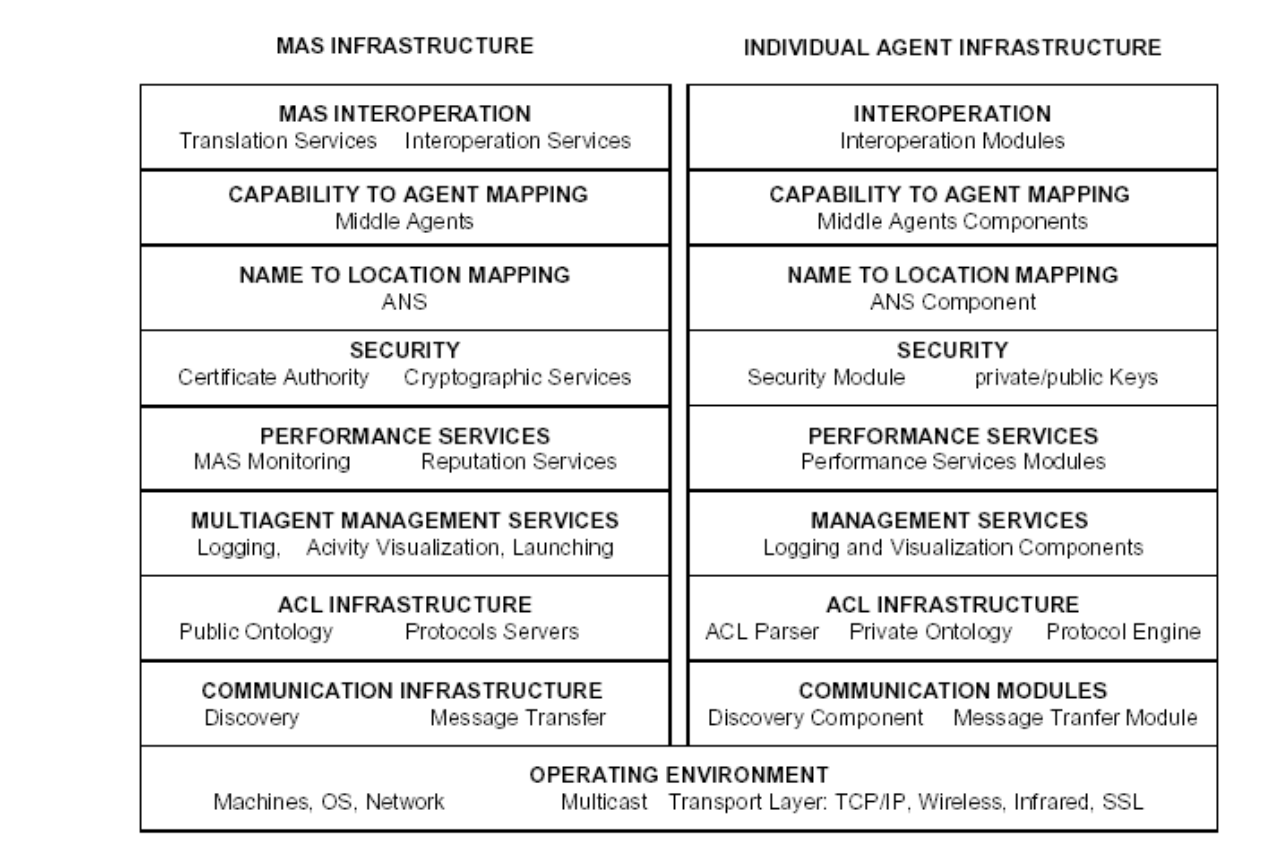
\includegraphics[width=.6\textwidth]{04/00}
\end{figure}

However, this is not a standard architecture, but rather a reference architecture that we can use in order to understand the kind of structures that can be included.\\
In particular, the structure of this architecture was proposed as a multi-layered architecture which includes a \side{MAS Infrastructure} and a \side{Individual agent infrastructure}.

\section{Low-level architectures}
The low level of the proposed architectures/set of services, deals with communication and the communication infrastructure. And there are only two ways that this infrastructure can be implemented: Shared memory and message sending/passing.
In the former, we consider how we can communicate via some common  channel where everybody can read and write something. In the latter, one agent send a message to exactly the recipient(s).

This is two basic approaches that can be implemented in very different ways and at different levels.
\subsection{Blackboards}
A possible shared memory approach to MAS communication there is a \side{Blackboard Architecture}.\\
The metaphor at the core of this architecture is that a collection of intelligent agents gather around a blackboard, loot at pieces of information written on it, think about them, and add their conclusions.

It means that each agent can only communicate via the blackboard.

Some basic assumptions of this method are 
\begin{itemize}
\item all of the agents can see all of the blackboard all the time, and what they see represents the current state of solution.\\
All information in the blackboard is available to all agents.
\item any agent can write his conclusions on the blackboard at anytime without gettin in anyone else's way.\\
The write operation is atomic and asynchronious.
\item the act of an agent writing on the blackboard will not confuse any other agents as they work.
\end{itemize}
The idea of blackboard architecture was originally implemented for translation of natural language.

The key ideas of the blackboard architecture is that problem solving should be:
\begin{itemize}
\item \side{Incremental}: complete solutions are constructed piece by piece, first hypothesizing a partial solution based on incomplete data and then attempting to verify additional data to verify hypothesis.\\

Agents do not just write whatever they want but rather they try to solve a problem (the solution to the problem is constructed incrementally).
\item \side{Opportunistic}: the system chooses the actions to take next that it determines will allow it to make the best progress towards meeting its goals in the current situation.\\

Having just a blackboard is not enough to solve a given problem, but there must be some organization mechanism on how to read, write and choose the next action. In other terms in order to solve the problem, the MAS must choose the most informative and useful element written in the balckboard
\end{itemize}
In figure \ref{fig:0401} a schematic representation of the blackboard architecture is proposed.
\begin{figure}[!h]
\centering
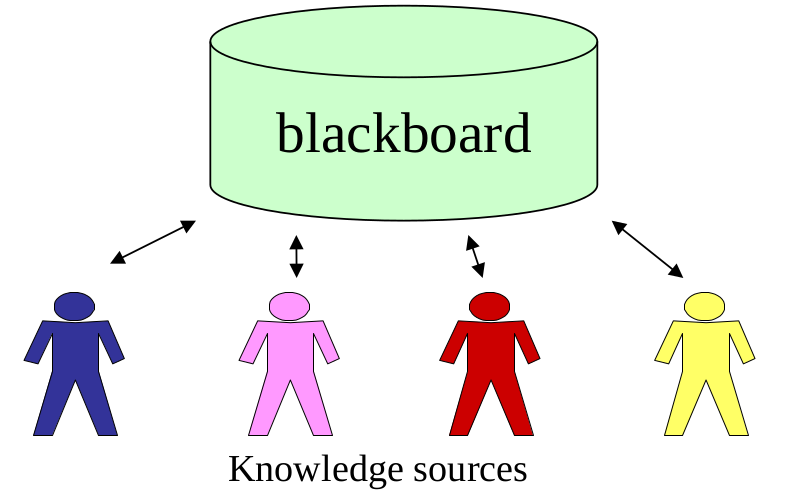
\includegraphics[width=.5\textwidth]{04/01}
\caption{}
\label{fig:0401}
\end{figure}

From the basic representation of the blackboard architecture we can identify the following main components:
\begin{itemize}
\item A \side{blackboard}: a global database containing data and hypotheses (potential partial solutions). 
\item A set of \side{Knowledge Sources (KS)} or agents
\item A \side{Control mechanism}, which will say what happens after an agents write something on the blackboard or that will decide who is going to be the next source of information.
\end{itemize}

The main control problem then is that of selecting the best action to execute next.

Blackboard systems, in fact, must have some control mechanism:
\begin{itemize}
\item allow effective control requires to take into account
\begin{itemize}
\item \side{Goal-directed factors}: based on what an agent wants.
\item \side{Data-oriented factors}: based on what an agent is best able to do. (based on what is written in the blackboard)
\end{itemize}
\item Blackboard control is difficult because it can be difficult to determine the expected value of an action by an agent as there may be complex interrelationships among the agents.
\end{itemize}

Before going into depth of the application of the blackboard architecture there is one important hypothesis that need to be considered: the \side{Serialisation Hypothesis}.\\
In principle, the idea is that agents can read and write whenever they want, but this is not efficient because there must be some kind of order in which agents can do this. \\
Such order is ensured by some serialisation:
\begin{itemize}
\item agents are schedulable entities and only one can be running at any time.
\item The control mechanism selects only the most productive agent at any given moment to work on the problem.
\item The blackboard is not gloabally visible. Agents generally work on a limited area of the blackboard, known as the agent's context.

In fact in principle agents have access to all the information of the blackboard, however for an efficiency point of view, it is better if agents look only into some locations.
\item Implicit assumption: a knowledge source/agent operates within a valid, or consistent context.
\end{itemize}

\subsubsection{Agenda-based Control}
A first type of Blackboard architecture that we consider is the \side{Agenda Base Control}.
\begin{figure}[!h]
\centering
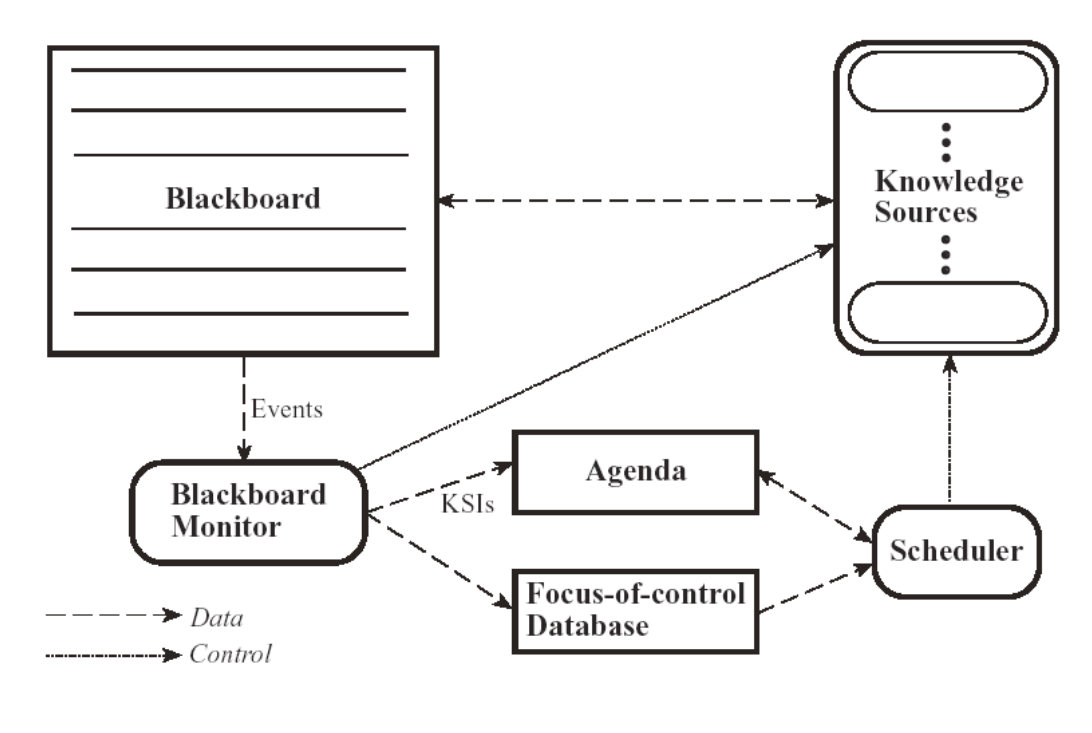
\includegraphics[width=.5\textwidth]{04/02}
\end{figure}
\begin{enumerate}
\item Each agent can write into Blackboard, and the act of writing generates some event. 
\item The event is then processed by some Blackboard monitor: a component that monitor what is going on in the blackboard and what should be the reaction.
\item When something new happears, the Blackboard monitor select what are other agents to whom this information may be useful.\\
\item Such information will be sent directly to the selected agents as a part of a preconditions for their execution. 
\item The selected agents will be put into an agenda to be scheduled for execution.
\item They way agents are selected from the agenda is through a rating which is attributed to each agent via a Focus-of-control database .\\
The task of this component  is to rate the execution of agents in the agenda based on the information and some other criteria.
\end{enumerate}
In the basic agenda-based blackboard architecture, all the control (strategy) knowledge of the system is represented in a single scheduler rating function.\\
This makes it difficult to encode and modify complex control strategies.\\
The knowledge and reasoning are not explicit.

\subsubsection{Event-based Control}
There are some alternative and modification of this type of control. When there may be not just one but many Event list that are triggered by the blackboard.
\begin{figure}[!h]
\centering
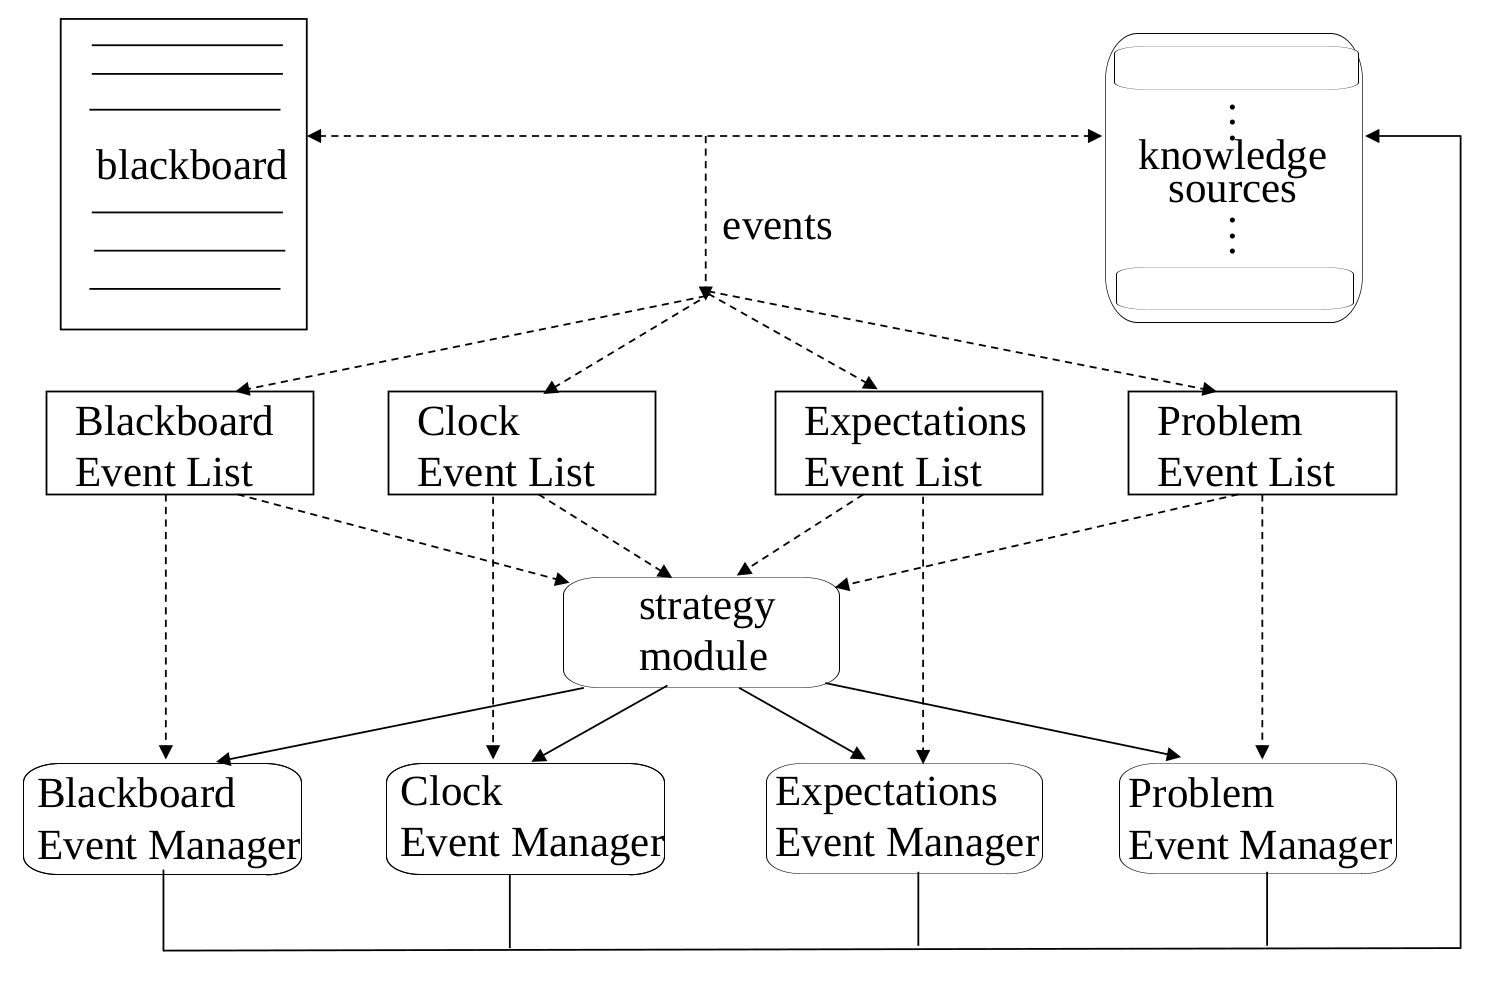
\includegraphics[width=.5\textwidth]{04/03}
\end{figure}
\begin{enumerate}
\item An agent write to the blackboard and an event is generated
\item Such event is then classified based on some property. This differentiate and classify what the agents is writing on the blackboard, which might be a general information, an expectation or a problem.
\item From the chosen amount of blackboard monitor there will be some strategy module, who decides from which event list to choose from.
\item A particular monitor/manager will handle the resulting event and transmit it to knowledge sources.
\end{enumerate}

\subsubsection{Goal-directed Control}
\side{Goal-directed control} considers the role and the ultimate value of actions in satisfying the system's goals.

\begin{figure}[!h]
\centering
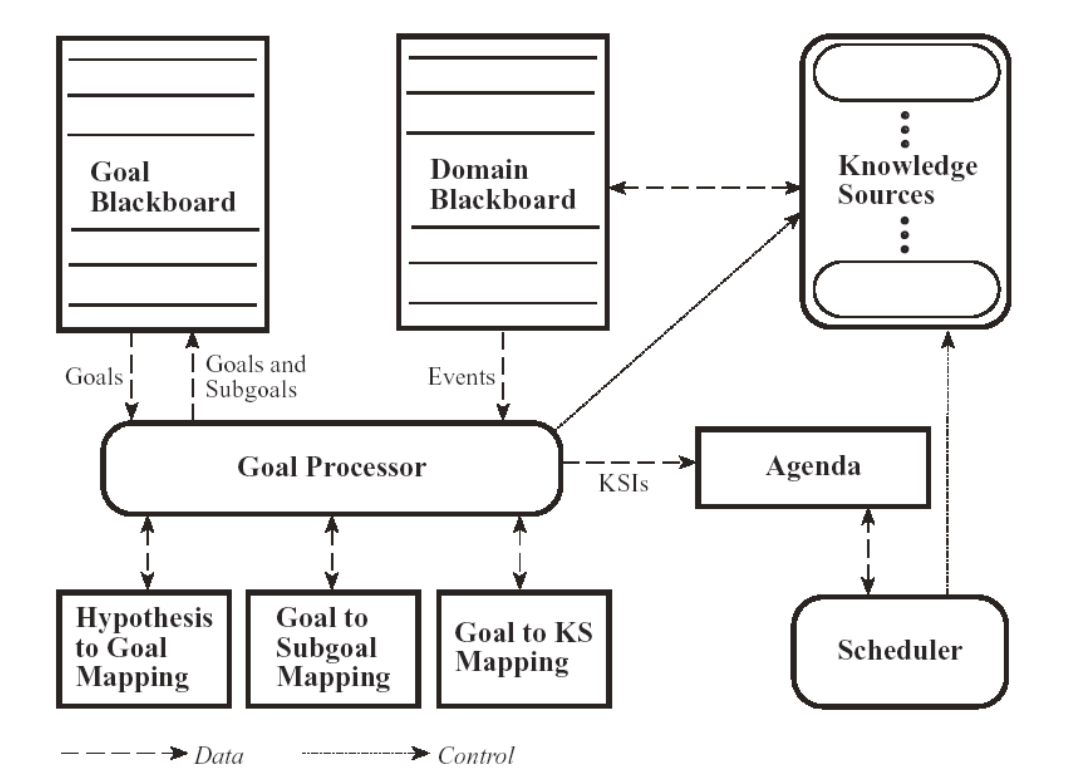
\includegraphics[width=.5\textwidth]{04/04}
\end{figure}
In this case there are two blackboard, namely a \side{Domain Blackboard} and a \side{Goal Blackboard}

\begin{enumerate}
\item An agent writes on the Domain Blackboard and generates an event
\item The goal processor processes information in the blackboard and transmit it to a particular agent and schedule such agent to execute via a scheduler.\\
In addition, the goal processor maps the event into a goal balckboard, whenever it cannot identify a specific agent to convey such information to.\\
From the goal blackboard some subgoals can be generated until an agent is found according to what we need.

This is some sort of reasoning mechanism that yields a more elaborated processing of each goal.
\end{enumerate}

Goal processor instantiates goals on the goal blackboard. Goal processor is driven by the 3 mapping functions. Integrates goal-directed and data-directed factors:
\begin{itemize}
\item Goal-directed goals are created in response to the creation of other goals based on the goal-to-subgoal map
\item Data-directed goals are created in response to the creation or modification of hypotheses on the blackboard based on the hypothesis-to-goal map
\end{itemize}

When a goal is inserted onto the goal blackboard, it may trigger KSs that can achieve the goal identified by the goal-to-KS map.\\
If KS is likely to generate a hypothesis to achieve the goal, KS is added to the agenda.\\
A possible problem may emerge: subgoaling needs to be carefully controlled.



\subsubsection{Hierarchy of Blackboard Servers}
Moreover, we can consider that the blackboard architecture is in reality a distributed blackboard, since keeping a centralized blackboard for every agent in the MAS can be a bottleneck.

However, by creating an hierarchy or a distributed system of blackboard. Between which some relations and dependecies exist.

\begin{figure}[!h]
\centering
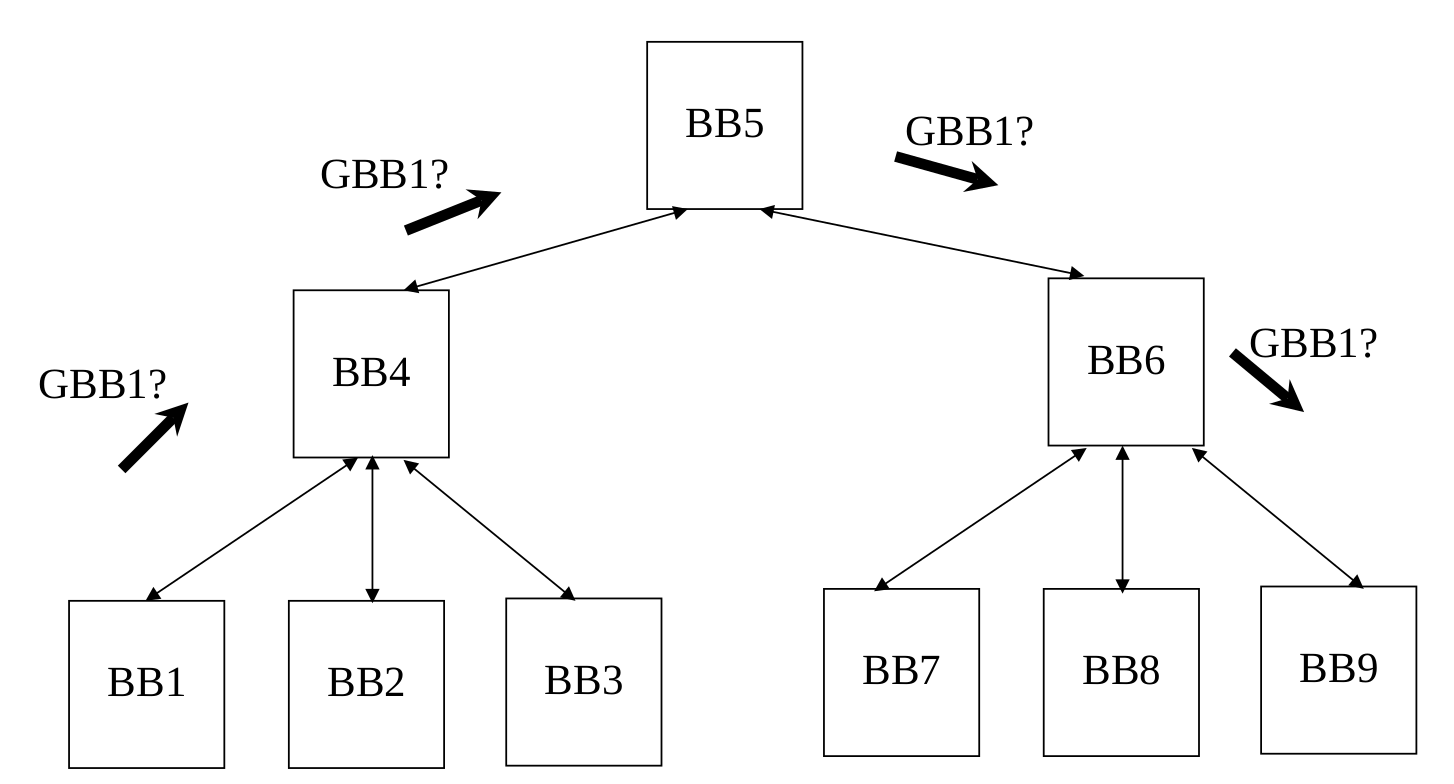
\includegraphics[width=.5\textwidth]{04/05}
\end{figure}

Whenver a goal gets written into a blackboard but there are no sources that can be find to understand what the next action should be, it will be forwarded to the upper level blackboard.
Such parent blackboard will see information and identify a blackboard that can process the information.
If yet there is no one that can process the information it will forward the goal to its parent blackboard and repeat the process.

\subsection{ACTORs}
ACTOR model approach is a pure message passing architecture that has the following properties
\begin{itemize}
\item \side{Social}, can send messages to other ACTORs
\item \side{Reactive}, carry out computation in response to a message received from another actor
\end{itemize}
In the ACTOR model, computation itself is viewed as message passing.
It can be considered as consisting of:
\begin{itemize}
\item An address
\item A behaviour which specifies what the ACTOR will do upon receipt of a message
\end{itemize}
In other term, we have some agents to be considered as a reactive entity, that has an address and a behaviour. Whenever an agent receives a message it executes its behaviour. As such agents are programs that can be triggered and have some address that we can invoke directly.

The ACTOR approach is formulated around three main design objectives:
\begin{enumerate}
\item Shared, mutable data. \\
Not shared channel but shared channels. This can be some kind of common data that all agents need in order to perform some kind of communication.
\item Reconfigurability.\\
New agent can be created and it is possible to communicate with such new agents.
\item Inherent concurrency.\\
Asynchronius behaviour is possible.
\end{enumerate}

An ACTOR is an object that carries out its actions in response to communication it receives.\\
ACTOR may perform only three basic actions:
\begin{itemize}
\item Sending messages to itself or other ACTORs
\item Creating more ACTORs
\item Specify a replacement behaviour, which is essentially another actor that takes the place of the actor that creates it, for the purpose of responding to certain communications.
\end{itemize}

The behaviour of an ACTOR model system is as follow:
\begin{itemize}
\item Upon receipt of a message, the message is matched against the ACTOR's behaviour (script)
\item Upon a match, the corresponsing action is executed, which may involve:
\begin{itemize}
\item Sending more messages
\item Creating more ACTORs
\item Replacing the ACTOR by another
\end{itemize}
\end{itemize}

ACTOR computation is therefore reactive.\\
An ACTOR is dormant until it receives communication.\\
In any computation, each ACTOR receives a linearly ordered sequence of computations.\\
Messages are not guaranteed to arrive in the order in which they are sent\\
There is no assignment to local variables in basic actor model\\
Every communication must be sent to a mail address: mail system is an important part of the model.

The communication event in actor model is called a task and it has 3 parts:
\begin{enumerate}
\item A unique tag, distringuishing it from tasks in the system
\item A target, the mail address of intended receiver
\item A communication which is the data passed by this communication event
\end{enumerate}

Actor model is asynchronous.\\
Communication is:
\begin{itemize}
\item explicity, through mail addresses, without shared variables 
\item buffered and asynchronous
\end{itemize}
Weak fairness is assumed:
\begin{itemize}
\item every message which is sent is eventually delivered
\item every computation eventually progress (no starvation)
\end{itemize}

\begin{figure}[!h]
\centering
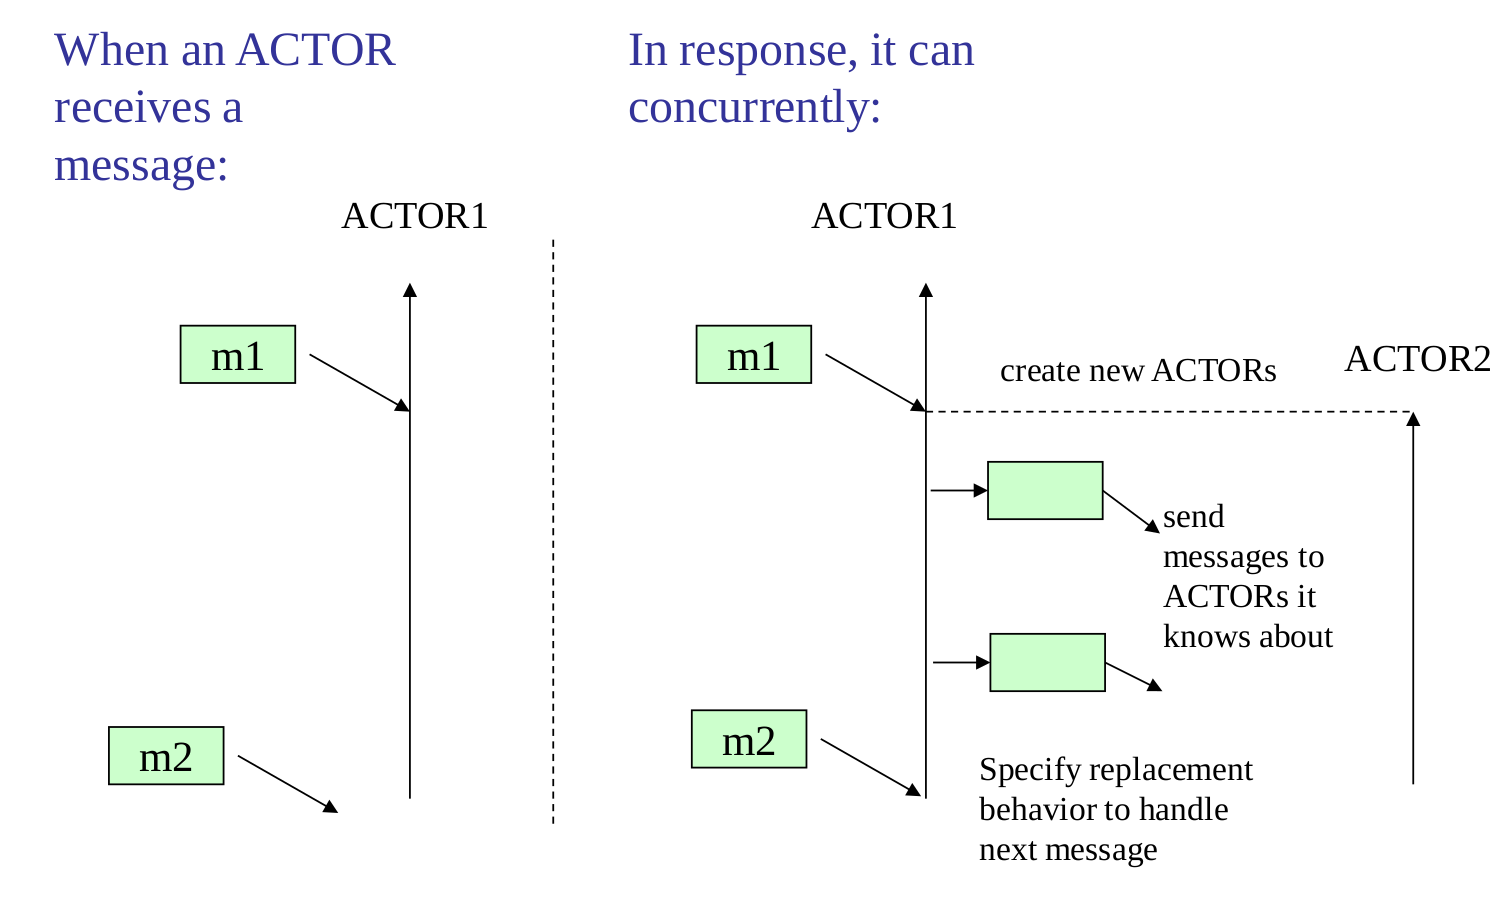
\includegraphics[width=.5\textwidth]{04/06}
\end{figure}


\subsubsection{Message sending based architecture: Agent Factory}
A few words about basic principles of Agent Factory:
\begin{itemize}
\item Linear discrete model of time which can be visualized as a sequence of numbers
\item A guaranteed delivery assumption. Messages are delivered correctly: the content of the message does not change in transaction, the message is sent to destinations and only to them
\item For any message there is only one sender
\item In spite of process synchronization: communication is asynchronous via message pool
\end{itemize}

\begin{figure}[!h]
\centering
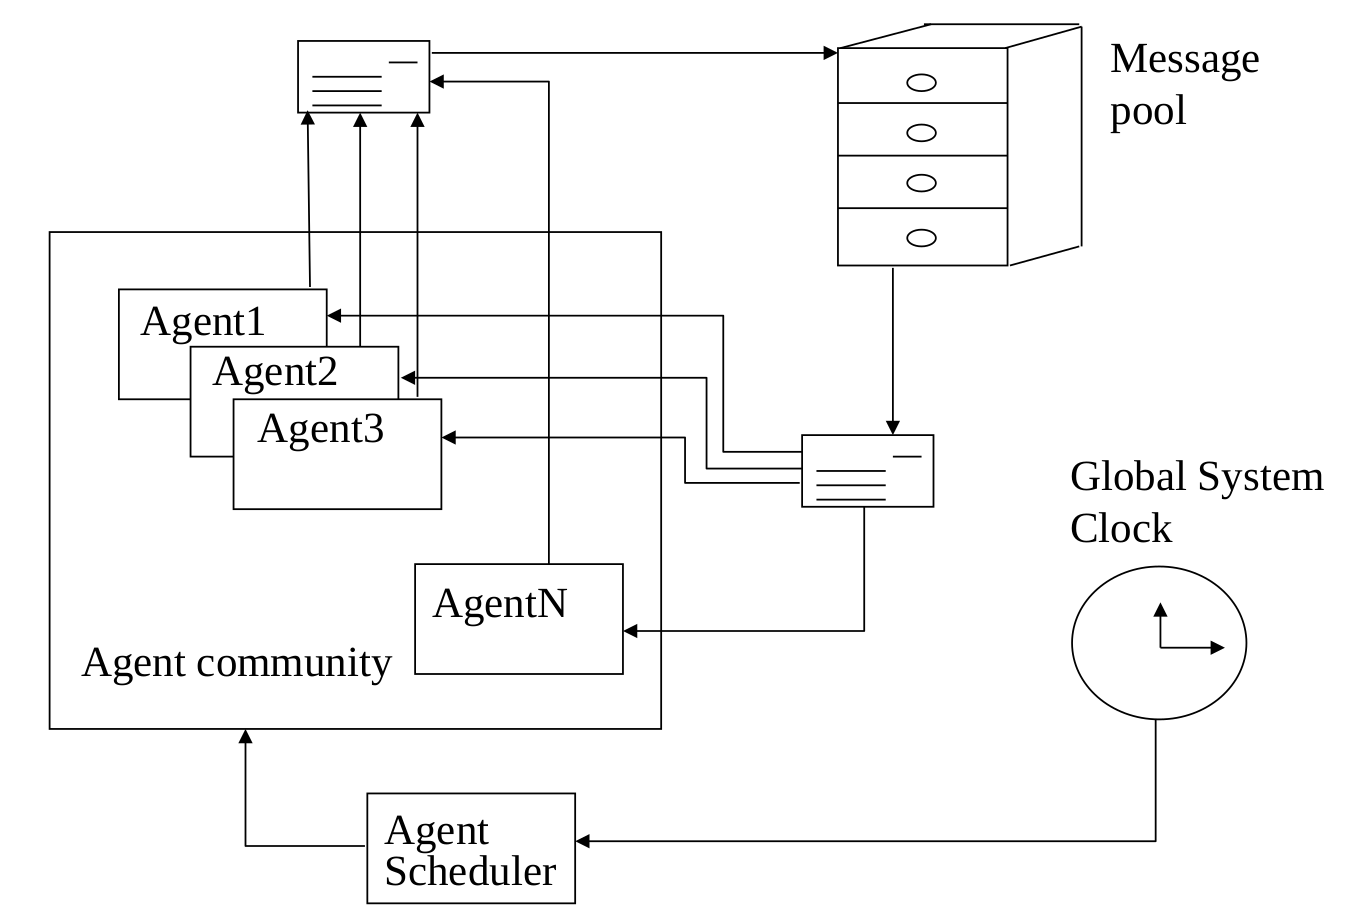
\includegraphics[width=.5\textwidth]{04/07}
\end{figure}

\section{Testbeds}
\side{Testbeds} are high-level architectures, which where developed specifically in the DAI community.\\
The main purpose of DAI testbeds is to support the implementation of ideas so that they can be evaluated in a useful context. In other terms, if a designer would like to propose a new algorithm for communication and negotiation, it can compare it with other algorithms via a testbed: this will allow to use the same example, the same tasks and the same system.

In order to have such a possibilities most DAI testbeds provide three classes of facilities to compare different class of algorithm:
\begin{itemize}
\item \side{Domain facilities}: representation and simulation of the problem being solved
\item \side{Development facilities}: an environment or tools for building the agents that will solve the problem
\item \side{Evaluation facilities}: tools for display, data collection, and analysis to understand how well the agents perform
\end{itemize}

\subsection{DVMT}
The \side{Distributed Vehicle Monitoring Testbed (DVMT)} is a DAI testbed developed to successfully track a number of vehicles that pass within the range of a set of distributed sensors (agents).

\begin{figure}[!h]
\centering
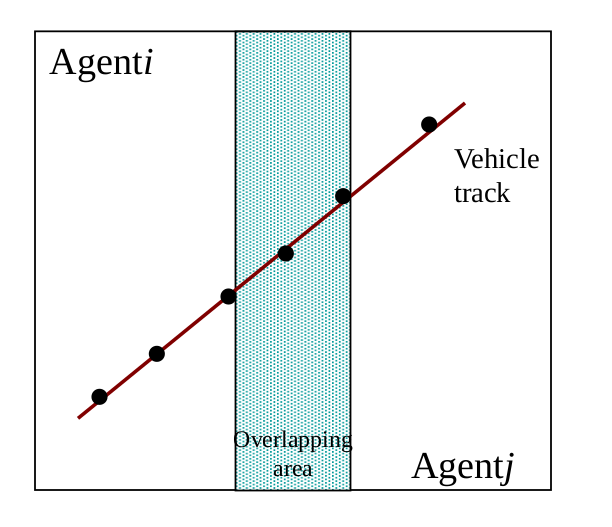
\includegraphics[width=.5\textwidth]{04/11}
\end{figure}

DVMT is a problem dependent testbed and agents (problem solvers) have a blackboard architecture.

\subsection{MACE}

MACE provides tools for constructing DAI systems at different level of abstraction with agents that have an ACTOR model:
\begin{itemize}
\item Each rule can be an agent
\item coarse-grained systems with large scale agents
\end{itemize}
MACE had no fixed domain for problem solving activity, however it have some fixed examples. 

\section{Infrastructures that use wrappers: ARCHON}
In many industrial applications, a substantial amount of time, effort and money was spent on developing complex and shophisticated software systems (e.g. expert systems and databases).\\
The basic idea is that we have a legacy system and we would like that these systems operate in a new environment. In order to do so, the designer could provide them with a wrapper that enable them to use in any other agent system.

This is what was implemented in \side{ARchitecture for Cooperative Heterogeneous ON-line systems (ARCHON)} was (in 1996) Europe's largest project in the area of DAI.\\
It was originally focused on getting a number of expert systems to pool their expertise in solving problems and diagnosing faults in several industrial domains.\\
Supports a cooperating community that has decentralized control and individual problem solving agents.\\
Consists of a:
\begin{itemize}
\item \side{Framework}: which provides assistance for interaction between constituent subcomponents
\item \side{Methodology}: which provides a means for structuring these interactions
\end{itemize}

ARCHON's individual problem solving entities are agents; they have the ability to control their own problem solving and to interact with other community members\\
Agents are large grain loosely coupled and semi-autonomous.\\
Each agent consists of an \side{ARCHON Layer (AL)} and an application program (known as \side{Intelligent System (IS)})\\
The ISs can be heterogeneous as their differences are masked by a standard AL-IS interface.\\

\begin{figure}[!h]
\centering
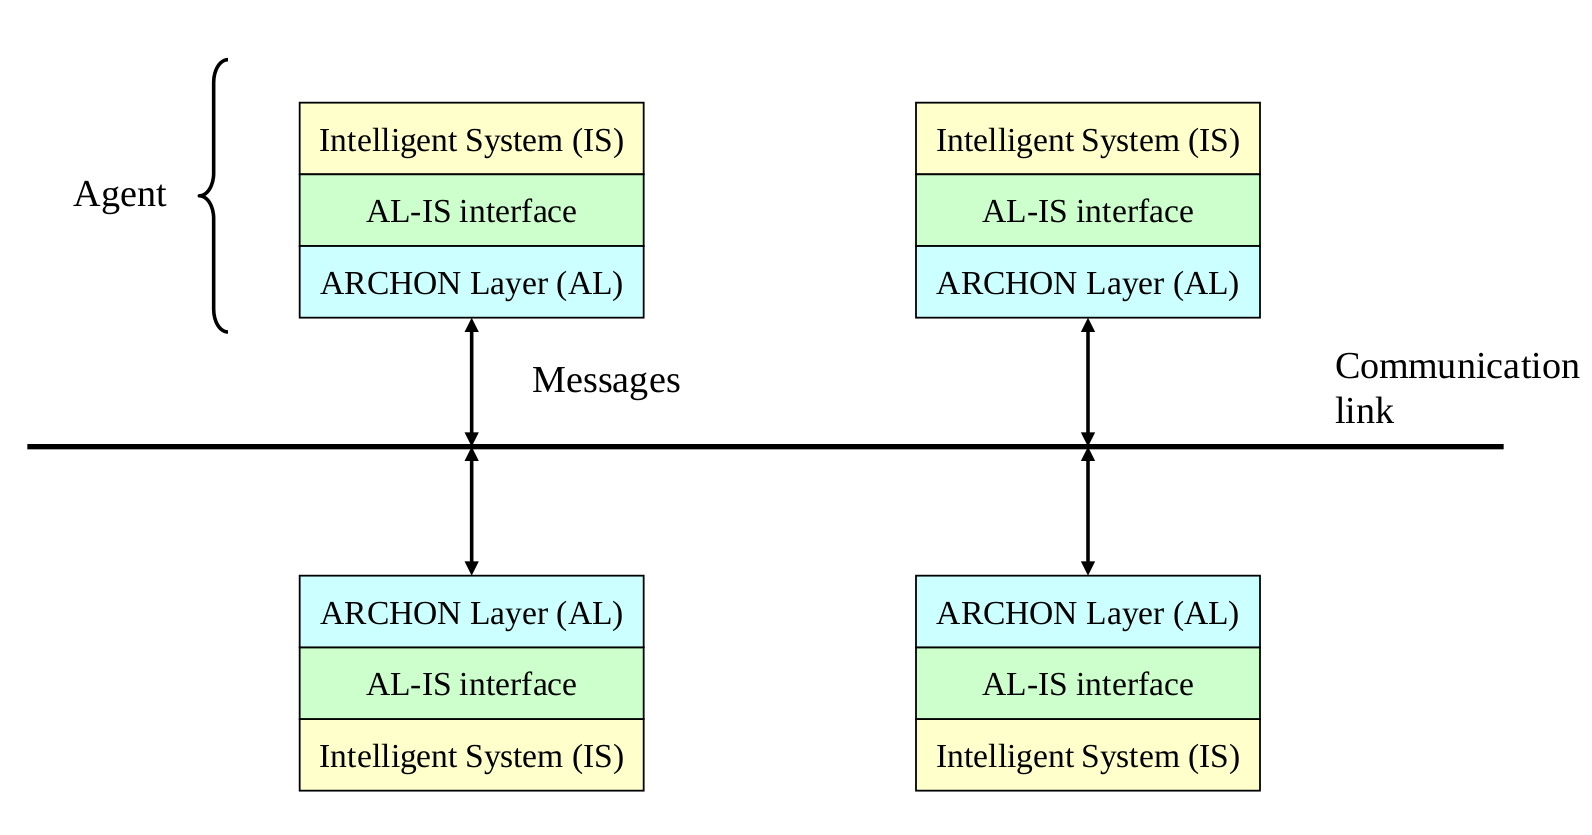
\includegraphics[width=.5\textwidth]{04/08}
\caption{}
\label{fig:archoncommunity}
\end{figure}

Figure \ref{fig:archoncommunity} shows the basic ARCHON community structure. Each agent has an:
\begin{itemize}
\item ARCHON layer that is responsible for the implementation of interagent communication and other services that are necessary for communication
\item An interface layer that allow the designer to wrap the Intelligent System into the overall MAS.
\end{itemize}
Communication happens via a single communication link or bus. This is fairly similar to KQML system where the Archon layer was the router, the AL-IS interface is similar to KRIL and lastly the intelligent system was the system itself.

This is a more general way of implementing a communication system where we define a set of general features that can be used by other system to communicate with the ARCHON Layer. This implies that it does not matter how we implement our Intelligent System, the communication will be consistent.

The most interesting part is how the AL-IS interface is structured, because it does not consist of a simple API, but more advanced techniques.

The system's overall objective is expressed in the separate local goals of each agent.\\
Agents' goals are usually interrelated. Therefore, social interactions are required to meet gloabl contraints.\\
Such interactions are controlled by the ARCHON layer which functions are to:
\begin{itemize}
\item Control tasks within the local IS
\item Decide when to interact with other agents (it needs to model the capabilities of its own IS as well the ISs of the other agents)
\item Communicate with other agents
\end{itemize}

\begin{figure}[!h]
\centering
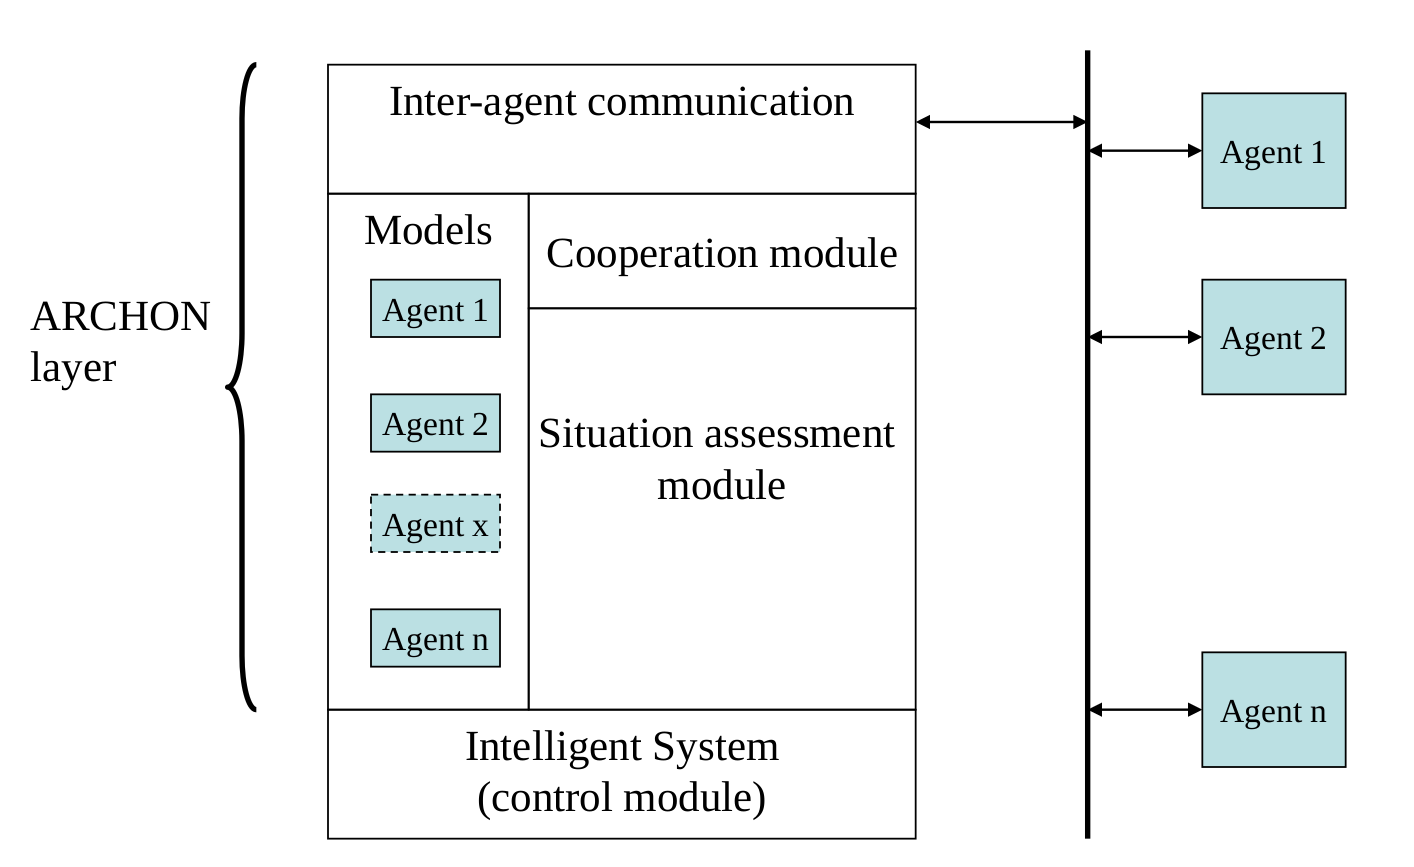
\includegraphics[width=.5\textwidth]{04/09}
\end{figure}

Looking into the three basic layers of the ARCHON architecture/approach we can notice that the ARCHON Layer can be devided into several modules:
\begin{itemize}
\item An Inter-agent communication layer/module that is responsible for supporting communication
\item An interface which is a set of components that can be adjusted in order to plugin the Intelligen System.

Among these modules we might find a \side{Cooperation module}, a \side{Situation assessment module} (something that you can tune in order to adjust your system), a set of Models of other agents or of itself.
\end{itemize}

In other terms this is a basic implementation that you can adjust in order to plugin the desired legacy system or intelligent system. It is a smooth translation model to some generic agent architecture.

\section{Infrastructures that use Middle Agents: RETSINA}
The idea of Middle agents is that instead of having a direct mechanism, Middle agents is a highly intelligent blackboard that it is implemented as shared memory but rather as an agent that can keep relationships between tasks and requests and proposals.

\begin{figure}[!h]
\centering
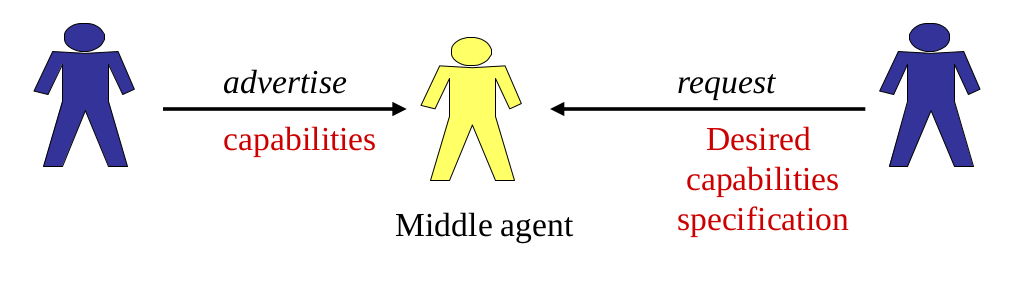
\includegraphics[width=.5\textwidth]{04/10}
\end{figure}

In an open system, the set of agents is not known a priori.\\
The infrastructure should provide ways for its agents to locate each other based on name, functionality or capability.

Agents that provide this service are called Middle agents which may also take the role of Facilitators or Matchmakers.

\side{REusable Task Structure-based Intelligen Network Agents (RETSINA)} is an open MAS infrastructure that supports communities of heterogeneous agents.\\
The main idea of RETSINA is that agents should form a community of peers that engage in peer-to-peer relations.\\
There is no central control and it implements distributed infrastructural services that facilitate the relation between agents.

RETSINA actually implements all the layers proposed in the reference architecture at the beginning of this chapter except for the interoperation layer.

\begin{figure}[!h]
\centering
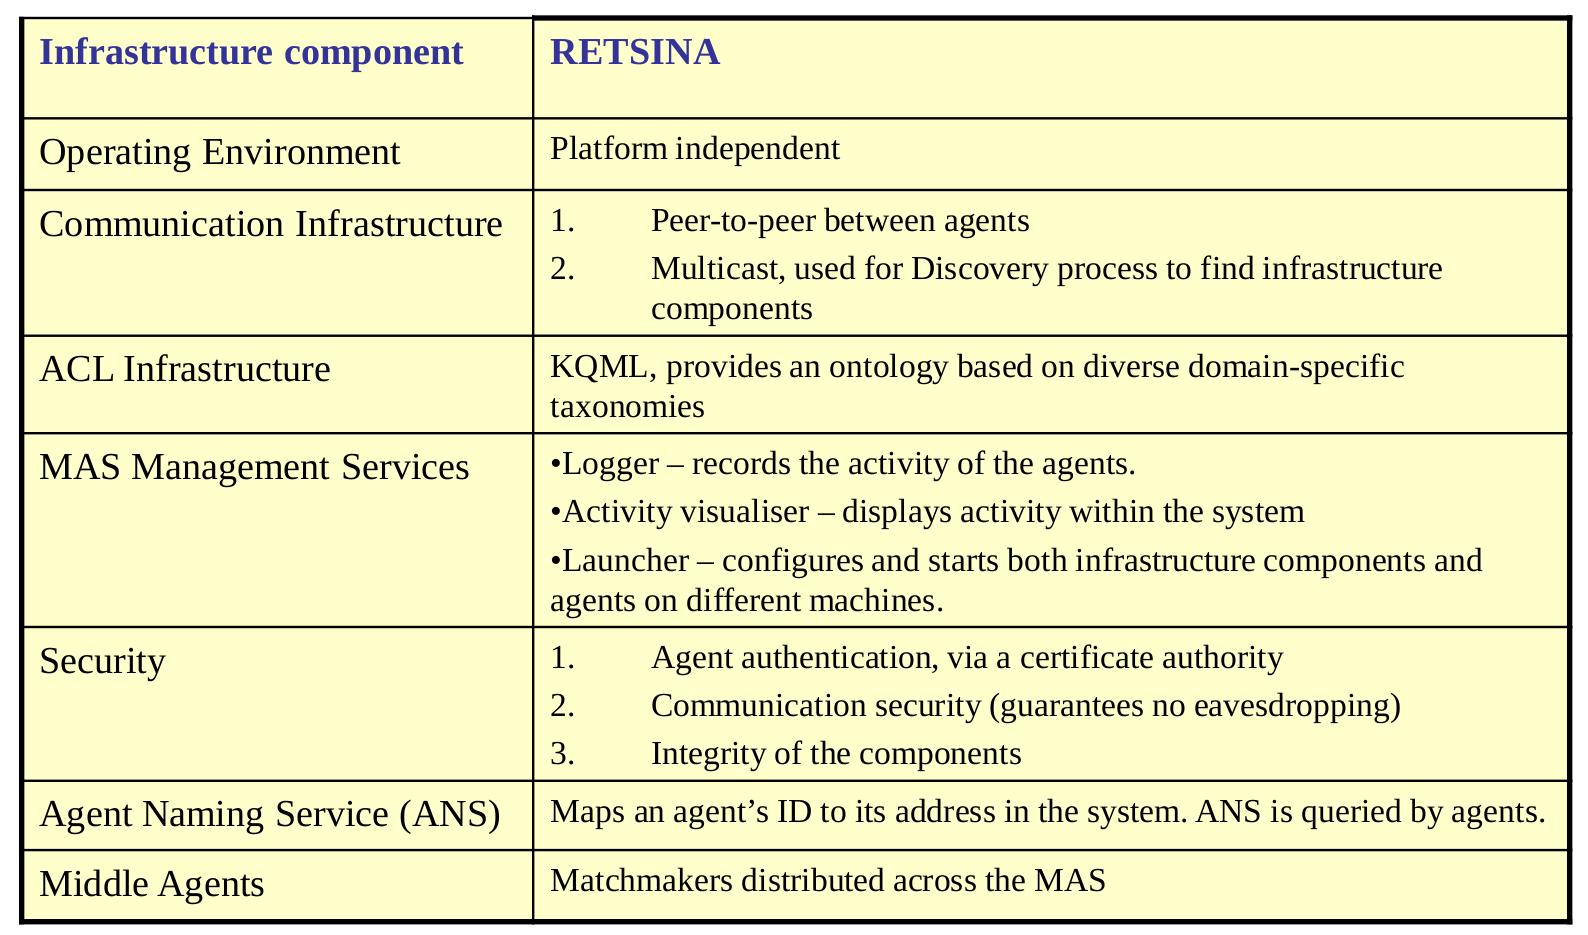
\includegraphics[width=.8\textwidth]{04/12}
\end{figure}

RETSINA middle agents are called Matchmakers, i.e. information agents that look for other agents rather than information:
\begin{itemize}
\item Records a mapping between agents in the system and the services they provide
\item Two types of data: advertisements and requests
\item the task of matchmakers is to match advertisements to requests
\item Two types of protocols: single shot and monitor
\end{itemize}


\section{Market-based architectures}
Online market places offer an opportunity to buyers and sellers to meet electronically and conduct trade. In some sense, these architecture consider a Middle agent to conduct their activity, but a special one which is the market place itself.

Offers benefits for both buyers and seller:
\begin{itemize}
\item Buyers: ease to process of searching for and comparing sellers
\item Sellers provide access to much broader customer bases
\end{itemize}

The major challenges are:
\begin{itemize}
\item to go beyond simple buying and selling
\item to incorporate time constraints, enforce deadlines, interact with a highly distributed web of suppliers with different capabilities and resources, interact over long periods of time and deal with failure in contract execution
\end{itemize}

The requirements of a Market-based Architecture are to:
\begin{itemize}
\item Provide support for a variety of transaction types (buying and selling, complex multi-agent contract negotiation, auctions)\\
This mechanism should be oriented towards different type of transactions.
\item Control fraud and misrepresentation
\item Discourage counterspeculation
\item Provide for secure and private credit and payment mechanisms
\item Provide a language in which the rich array of semanting content about commerce can be expressed
\item Provide for robust exception handling
\item Scale smoothly from local to global
\item Be extensible, by third parties
\item Interoperate with other new and existing electronic commerce services
\end{itemize}
So the idea is that in addition to the standard Matchmaking propose-request we need to implement the aforementioned features.

\subsection{MAGNET}
The  \side{Multi-AGent NEgotiation Testbed (MAGNET)} is a testbed to support multiple agents in negotiating contracts.\\
Supports negotiation of contract for tasks that have temporal and precedence constraints.\\
Distinguishes between the agents:
\begin{itemize}
\item Customer: needs resources outside its direct control in order to carry out its plans
\item Supplier: provides the resources and services required by customers, for a specified price, over specified time periods
\end{itemize}

\begin{figure}[!h]
\centering
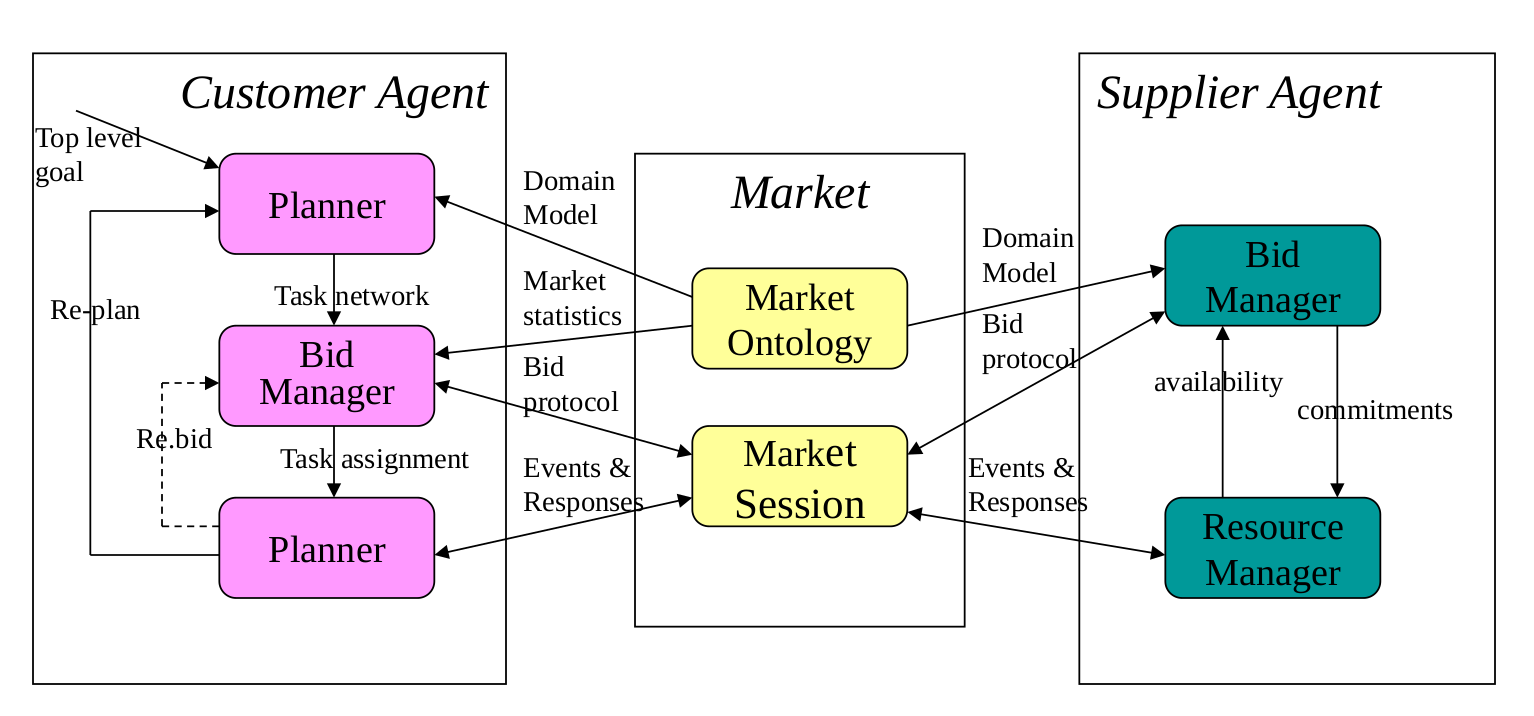
\includegraphics[width=.5\textwidth]{04/13}
\end{figure}

In this architecture there are:
\begin{itemize}
\item A special element called market that implements market sessions and may implement also Market Ontology or knowledge about such market place.
\item Customer agents, that are provided with a Planner in order to plan its task and a Bid Manager.
\item Supplier agent will have a Bid Manager and a Resource Manager.
\end{itemize}

In the general case, the bidding process goes as follows:
\begin{enumerate}
\item Customer agent plans a set of task
\item Getting information about the Market Ontology, the Customer Agent can create bids via the Bid Manager and publish such tasks to be performed into the Market Session
\item The Supplier Agent gets information about the Market Ontology and via the communication between the Bid Manager and the Resource Manager, decides which of the resources of interest are available.
\item Based on the information of availability derived from the Resource Manager, the Supplier Agent will publish into the Market Session
\item The bid protocol will coordinate the rules of the action or negotiation.
\item Depending on whether or not the bid was accepted or rejected, the Customer Agent may decide to rebid or replan its tasks.
\item Upon agreement the Supplier Agent will commit via the Resource Manager to provide the agent with the resources needed.
\end{enumerate}


The interaction among agents goes as follows
\begin{enumerate}
\item A customer issues a Request for Quotes (RFQ), which sp[ecifies tasks, the precedence relations and a timelien for the bidding process
\item Supplier agents submit a bid, which includes a set of tasks, a price, a portion of the price to be paid as a non-refundable deposit and estimated timeline
\item The customer decides which bid to accept based on cost, risk and time constraints
\item The customer awards bid, notifies the suppliers of their commitments and specifies the work schedule
\end{enumerate}

The interactions between the customer and supplier agents are encapsulated in a market session. The market session:
\begin{itemize}
\item finds suppliers interested in bidding for the customer
\item provides a catalog of services (market ontology)
\item time-stamps all the interactions in order to avoid dispute among customers and suppliers
\end{itemize}

\begin{figure}[!h]
\centering
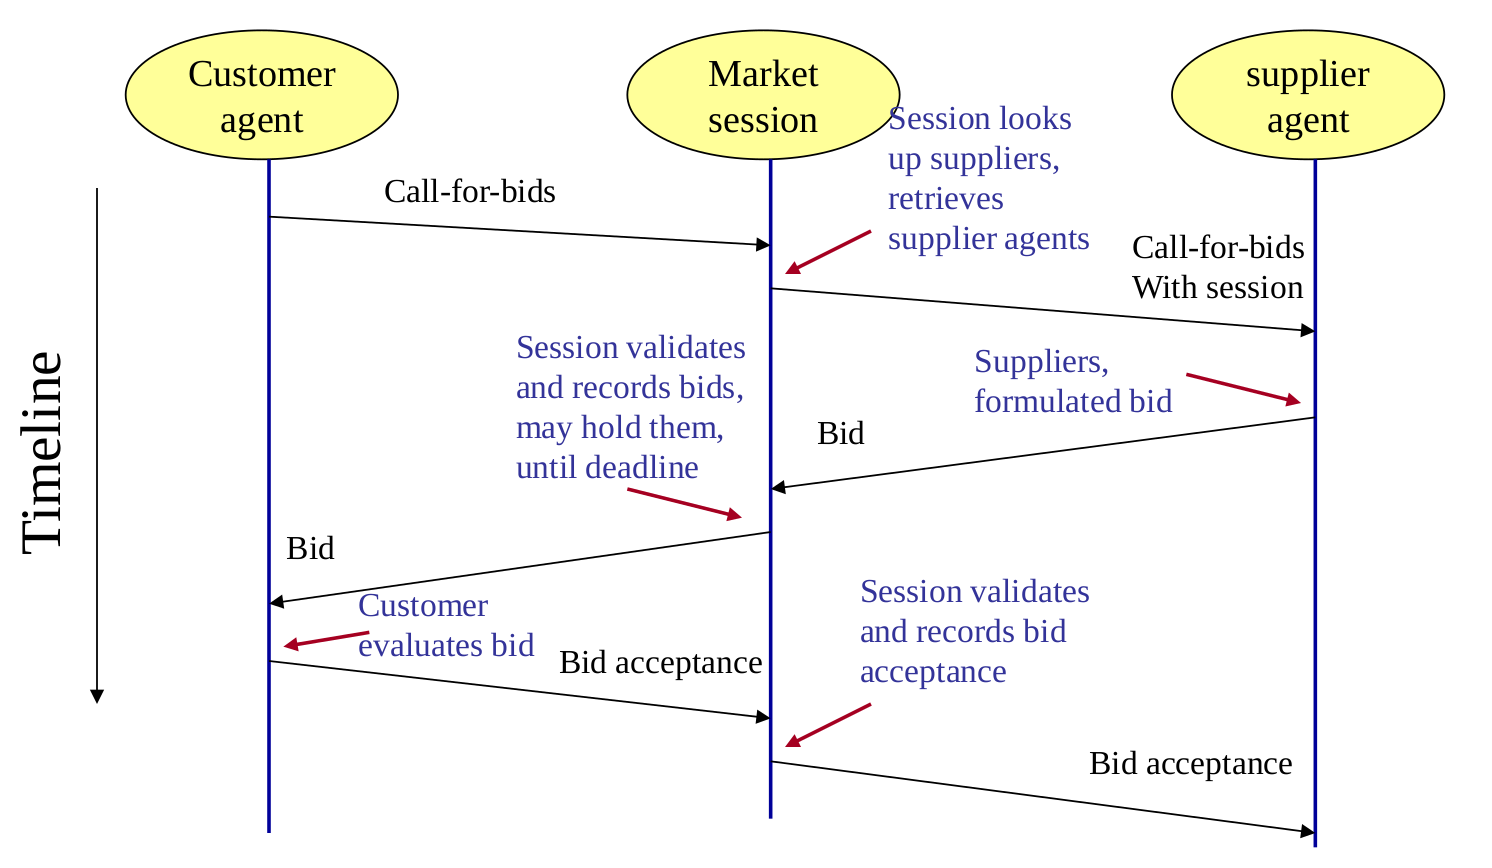
\includegraphics[width=.5\textwidth]{04/14}
\end{figure}

The session:
\begin{itemize}
\item Truthfully informs the suppliers of the conditions under which the bidding is being done and enforces these conditions
\item Can limit the number of bids sent by each supplier
\item May provide information about suppliers to customers
\item Enforces the rules of the market
\item Can act as a trusted auctioneer
\end{itemize}

\section{Conclusion}
We consider our MAS infrastructure as middleware on the top of system software.
Cooperative work support is an important element of the infrastructure and it needs conceptual solutions
Extensibility and default components are important features
We should be as much as possible close to standards (if they do not exist then to general tendencies)




    \chapter{Agent Oriented Software Engineering}
\minitoc

As MASs become more established in the collective consciousness of the computer science community, we might expect to see increasing effort devoted to devising methodologies to support the development of agent systems.

\section{When is an Agent-Based Solution Appropriate?}

There are a number of factors which point to the appropriateness of an agent-based approach:
\begin{itemize}
\item The environment is open or at least highly dynamic, uncertain or complex
\item Agents are a natural metaphor.\\
Many environments are naturally modelled as societies of agents, either cooperating with each other to solve complex problems, or else competing with one another.
\item Distribution of data, control or expertise.\\
In some environments, the distribution of either data, control or expertise means that a centralized solution is at best extremely difficult or at worst impossible.
\item Legacy systems.\\
A problem increasingly faced by software developers is that of \side{legacy software}, that is technologically obsolete but functionally essential to an organization.\\
Such software cannot generally be discarded, because of the short-term cost of rewriting. And yet it is often required to interact with other software components which were never imagined by the original designers. One solution to this problem is to wrap the legacy components, providing them with an agent layer functionality, enabling them to communicate and cooperate with other software components.
\end{itemize}

\section{Agent-Oriented Analysis and Design}
An analysis and design methodology is intended to assist first in gaining an understanding of a particular system and secondly in designing it.\\
Methodlogies generally consist of a collection of models, and associated with these models, a set of guidelines. The models are intended to formalize understanding of the system being considered.

Analysis and design methodolgies of agent-based systems can be broadly divided into two groups:
\begin{enumerate}
\item Those that take their inspiration from OO development, and either extend existing OO methodologies or adapt OO methodologies to the purposes of \side{Agent-Oriented Software Engineering (AOSE)}
\item Those that adapt knowledge engineering or other techniques
\end{enumerate}
\subsection{The AAII methodology}
The \side{Australian AI Institute (AAII)} developed a range of agent-based systems using their PRS-based belief-desire-intention technology and the distributed  multiagent reasoning system (DMARS).

This methodoly draws primarly upon OO methodologies and enhances them with some agent-based concepts. The methology itself is aimed at the construction of a set of models which, when fully elaborated, define an agent system specification.

The AAII methology provides two types of model:
\begin{enumerate}
\item The \side{External model} presents a system level view: the main components visible in this model are agents themselves.

The external model is thus primarly concerned with agents and the relationships between them.\\
Particularly the external model is intended to define inheritance relationships between agents classes, and to identify the instance of these classes that will appear at run time.

It is itself composed of two further models: the \side{agent model} and the \side{interaction model}.

Furthermore the agent model is divided into an \side{agent class model} and an \side{agent instance model}. 

\item The \side{Internal model} is concerned with the internals of agents: their beliefs, desires and intentions
\end{enumerate}

These two models define the agents and agent classes that can appear, and relate these classes to one another via inheritance, aggregation and instantiation relations.
Each agent class is assumed to have at least three attributes: beliefs, desires and intentions. The analyst is able to define how these attributes are overridden during inheritance.
Details of the internal model are not given but it seems clear that developing an internal model correspons fairly closely to implementing a PRS agent.

The AAII methodology is aimed at elaborating the models described above. It may be summarized as follows:
\begin{enumerate}
\item Identify the relevant roles in the application domain and on the basis of these, develop an agent class hierarchy
\item Identify the responsibilities associated with each role, the services required by and provided by the role and then determine the golas associated with each service.
\item For each goal, determine the plans that may be used to achieve it and the context conditions under which each plan is appropriate
\item Determine the belief structure of the syste, the information requirements for each plan and goal.
\end{enumerate}
Note that the analysis process will be iterative, as in more traditional methologies. The outcom eiwll be a model that closely corresponds to the PRS agent architecture. As a result, the move from end-design to implementation using PRS is relatively simple
\subsection{The GAIA methodology}
The \side{GAIA methology} is intended to allow an anlyst to go systematically from a statement of requirements to a design that is sufficiently detailed that it can be implemented directly.

In applying GAIA, the analyst moves from abstract to increasingly concrete concepts. Each successive move introduces greater implementation bias and shrinks the space of possible systems that  could be implemented to satisfy the original requirement statement.
Gaia borrows some terminology and notation from OO analysis and design. However, it is not simply a naive attempt to apply such methods to Agent-oriented development. Rather, it provides an agent-specific set of concepts through which a software engineer can understand and model a complex system. In particualr, Gaia encourages a developed to thing of building agent-based systems as a process of \side{organizational design}.

The main Gaia concepts can be divided into two categories: 
\begin{itemize}
\item \side{abstract} entities are those used during analysis to conceptualize the system, but which do not necessarily have any direct realization within the system
\item \side{concrete} entities are used within the design process, and will tipically have direct counterparts in the run-time system.
\end{itemize}

The objective of the analysis stage is to develop an understanding of the system and its structure without reference to any implementation detail. In the Gaia case, this undestanding is captured in the system's \side{organization}.\\
An organization is viewed as a collection of roles that stand in certain relationships to one another and that take part in systematic, institutionalized patterns of interactions with other roles.

The idea of a system as a society is useful when thinking about the next level in the concept hierarchy: \side{roles}. A role is defined by four attributes: 
\begin{enumerate}
\item \side{Responsibilities}\\
They determine funcitonality and as such are perhaps the key attribute associated with a role.\\
Responsibilities are divided into two types:
\begin{enumerate}
\item \side{Liveness properties} descirbe those states of affair that an agent must bring about, given certain environmental conditions.
\item \side{Safety properties} are invariants, which in other terms states that an acceptable state of affairs is maintained across all states of execution.
\end{enumerate}
\item \side{Permissions}\\
A role has a set of permissions which identify the resources that are available to that role in order to realize its responsibilities. Permissions tend to \side{information resources}.
\item \side{Activities}\\
The activities of a role are computations associated with the role that may be carried out by the agent without interacting with other agents. activities are thus private actions.
\item \side{Protocols}\\
A role is also identified with a number of protocols, which define the way that it can interacti with other roles.
\end{enumerate}
\subsection{The Tropos methodology}
The \side{Tropos methodology} aims to give an agent-oriented view of software throughout the software development lifecycle.\\
It provides a conceptual framework for modelling systems based on the following concepts:
\begin{itemize}
\item \side{Actor}\\
An entity with strategic goals and intentionality within the system or the organizational setting.\\
Associated with actors are the notions of role and position.
\begin{itemize}
\item A role is an abstract characterization of the behaviour of a social actor within tsome specialized context
\item A position is a set of roles, typically played by one agent
\end{itemize}
\item \side{Goal}\\
A goal represent sthe actors; strategic interests. Tropos distinguish \side{hard goals} (system funcitonal requirements) and \side{soft goals} (non-functional requirements)
\item \side{Plan}\\
A recipe for achieving a goal.
\item \side{Resource}\\
Physical entities or information
\item \side{Dependency}\\
A relationship between two actors, indicating that one agent needs the other to carry out some part of a plan, deliver some resource, or similar
\item \side{Capability}\\
The ability of an actor to achieve some goal or carry out some plan
\item \side{Belief}\\
Knowledge that actors have about their environment.
\end{itemize}

The first phase of analysis in Tropos involves developing an :
\begin{itemize}
\item \side{actor model}, which captures the key stake holders in the system and their strategic intersts in the form of their goals 
\item \side{dependency model}, which documents the dependencies between these actors
\end{itemize}

A \side{goal model} is then developed, which decomposes goals into their constituent parts, and, associated with this, a \side{plan model} captures the structure of recipes for achieving goals.

\subsection{The Prometheus methodology}
The \side{Prometheus methodology} consists of three main stages:
\begin{enumerate}
\item \side{System specification}, which focuses on identifying the goals and basic functionalities of the system, and specifies the interface between the system and its environment in terms of actions and percepts
\item \side{Architectural design}, which focuses on identifying agent types, the system structure and the interactions between agents
\item \side{Detailed design}, which first involves refining agents into their capabilities and specifying the processes ion the system and then involves the detailed design of capabilities
\end{enumerate}
Prometheus provides a rich collection of models for each stage and detailed guideline for each step. It also has software tool support

\subsection{Agent UML}
The \side{Undefined Modelling Language (UML)} is an attempt by three of the main figures behind object-oriented analysis and design to develop a single notation for modelling OO systems.\\
It is important to note the UML is NOT a methodology, but rather a language for documenting models of systems; however, associated with UML is a methodology known as the rational unified process.

When looking for agent-oriented modelling languages and tools, many researchers felt that UML was the obvious place to start. The result has been a number of attempts to adapt the UML notation for modelling agent systems.\\
The proposed modifications include:
\begin{itemize}
\item support for expressing concurrent threads of interactino thus enabling UML to model such well-known agent protocols as the the Contract Net
\item A notion of role that extends that provided in UML and in particular allows the modelling of an agent playing many roles
\end{itemize}
Both the Object Management Group and FIPA are currently supporting the development of UML-based notations for modelling agent systems, and there is therefore likely to be considerable work in this area.

\subsection{Discussion}
The predominant appraoch to developing methodologies for MASs is to adapt those developed for OO analysis and design.
There are several disadvantages with such approaches:
\begin{itemize}
\item the kind of \side{decomposition} that OO methods encourage is at odds with the kind of decomposition that agent-oerinted design encourages.
\item OO methodologies simply do not allow us to capture many aspects of agent systems. The extensions to UML proposed address some, but by no means all of these deficiencies.
\item At the heart of the problem is the problem of the relationship between  agents and objects which has not yet been satisfactorily resolved.
\end{itemize}

\section{Pitfalls of Agent Development}

\begin{itemize}
\item \textbf{You oversell agent solutions, or fail to udnerstand where agents may usefully be applied}
\item \textbf{You get religious or dogmatic about agents}
\item \textbf{You do not know why you want agents}
\item \textbf{You want to build generic solutions to one-off problem}
\item \textbf{You believe that agents are a silver bullet}
\item \textbf{You forget that you are developing software}
\item \textbf{You forget that you are developing multithreaded software}
\item \textbf{Your design does not exploit concurrency}
\item \textbf{You decide that you want your own agent architecture}
\item \textbf{Your agents use too much AI}
\item \textbf{You see agents everywhere}
\item \textbf{You havce too few agents}
\item \textbf{You spend all your time implementing infrastructure}
\item \textbf{Your agents interact too freely or in a disorganized way}
\end{itemize}
    % ==============================================================
% File     : chapters/06-Theory.tex
% Date     : 03 Apr. 2022
% Revision : 30 July 2022
% Creator  : Marco Peressutti
% ==============================================================


\chapter{Agent Theory}
\minitoc

Previously we mainly considered agent group perspective in which agents communicate, negotiate and coordinate their activities.\\
In this section, we will focus on individual perspective of agents, in the sense of how agents operate in terms of theoretical model architecture and mobility for implementing their particular task.\\
The first element of this individual perspective is called \side{Agent Theory}.

The reason why it is necessary to consider agent theory and formalisms is because formal theory has arguably had little impact on the general practice of software development, however, they are relevant in agent-based systems because we need to be able to give a semantic to the architecture, languages and tools that we use (i.e. a meaning).\\
Moreover without a semantic, it is never clear exactly what is happening and why it works.\\
But most importantly we need a theory to reach any kind of profound understanding the tools.

On the other hand the formalization of agents can be seen from 2 distinct perspective/purposes:
\begin{enumerate}
\item As \side{internal specification language} to be used by the agent in its reasoning or action
\item As \side{external metalanguage} to be used by the designer to specify, design and verify certain behavioural properties of agents situated in a dynamic environment.
\end{enumerate}

Agent theory gives us both an overview of the ways in which an agent is conceptualised and semantics to the architecture, language and tools: in other terms, we strive to formalise and conceptualise what is an autonomous entity and what is an autonomous behaviour.\\
Of course in order to have a theory of agent we need to introduce or consider a model of agents. For this purpose we will consider agents as\side{intentional systems}: the behaviour of an agent is explained in terms of attitudes such as believing and wanting.

\section{Agents as intentional systems}
Theorists start from the notion of an agent as an intentional system.\\
So, agent theorists start with the view of agents as intentional systems: where agent's behaviour is explained in terms of \side{attitudes}.
\subsection{Attitudes}
Attitudes represent a summary evaluation of a psycological object (e.g. oneself, other people, issue, plan, behaviour). We do not know for sure how it works, but it is our perception and psychological understanding.
For this reason attitudes are formed throughout the interaction with the surrounding environment and help to manage individual's cognitive resources to deal with uncertainties of complex dynamic domains.

In fact, the knowledge of the environment is seldom precise, agents may not know for sure or the environment may change. In this sense the agent knowledge is based on some uncertain element which prevents us to use plane knowledge base system as a foundation for agent. Moreover,  when dealing with autonomous entities we need a way to generate goals. And attitudes enable agents to express the knowledge about the world, as well as intentions and goals, similarly to humans.

Formally an attitude is the use of a folk psychology, by which human behaviour is predicted and explained through the attribution of attitudes.\\
Human however, do not act on attitudes, but rather use the notion of attitudes to explain their action. This is the reason why this formalism was chosen as a way to describe agent behaviour.

The attitudes employed in such folk psychological descriptions are called \side{intentional notions}.\\
An approach is to describe agent's behaviour in terms of intentional systems, ``whose behaviour can be predicted by the method of attrivutring belief, desire and rational acumen''.

An intentional system could be quite complex: first-order (attitudes), second-order (reasoning about attitudes),... etc.

Given all of the above, we might ask ourselver: is it useful to consider agents (similar to humans) as intentional systems? John McCarthy claims that:
\begin{itemize}
\item It is legitimate when it express the same information about the machine that it expresses about a person. 
\item It is useful when it helps us understand the structure of the artifact
\item It perhaps never logically required even for humans. \\
In fact, humans do not operate according to intentional notions but rather use attitudes and intentional notions to explain their action.
\item Ascription of mental qualities is most straightforward for machines of known structure but most useful for entities whose structure is incompletely known.\\
In simpler terms, if we completely know how a system works, then intentional systems are NOT useful. But the point is that agents do not and in fact cannot know exactly how the system works.\\
The more we know about a system the less we need to rely on intentional explanations of its behaviour.
\end{itemize}
An autonomous agent is a system that is most conveniently described by the intentional stance since it tries to mimic the behaviour of human which we do not know. 
\subsection{Theories of Attitudes}
We want to be able to design and build computer systems in terms of mentalistic notions.
Before we can do this, we need to identify a manageable subset of these attitudes and a model of how they interact to generate system behaviour. So first, which attitudes?

There exists 2 categories of attitudes:
\begin{enumerate}
\item \side{information attitudes}: which express the perception of the world (e.g. belief and knowledge)
\item \side{Pro-attitudes}: which guides agents behaviour (e.g. desire, intention, obligation, commitment, choice...)
\end{enumerate}
In principle, a good approach would be to choose at least one attitude from both of the categories.

The manipulation of these attitudes falls in the study of knowledge.
\subsection{Study of Knowledge}
The study of knowledge tries to answer a series of open questions:
\begin{itemize}
\item What do we know?
\item What can we know?
\item What does it mean to say someone knows something?
\item What does an agent need to know in order to perform an action?
\item How does an agent know whether it knows enough to perform an action?
\item At what point does an agent know enough to stop gathering information and make a decision?
\end{itemize}
In other terms, it is of our desire to formalise the intentional system in such a way that agent can reason about it.

Moreover, we need to distinguish between two different dimensions of knowledge:
\begin{itemize}
\item Individual perspective
\item Group perspective, which encompasses the knowledge of other agents in the group, \side{common knowledge} (e.g. traffic rules) and \side{distributed knowledge} (agents hold only a small portion of knowledge but only together can come up with the whole knowledge)
\end{itemize}


\section{Foundation of formal logic}

The formalisation of attitudes and knowledge requires some logical theory at its core.\\
A \side{formal logic} is a game for producing symbolic objects according to given rules. It can be interpreted as a sort of language with some general syntax or alphabet which include the following notation:
\begin{itemize}
\item Variables ($X,Y, ...$)
\item Constants ($a, abc, 15, ...$)
\item Functors ($f/n$) or functional symbol
\item Predicate symbols ($p,q,...$)
\item Logical connectivities ($\neg, \lor, \land, \rightarrow, \iff$)
\item Quantifiers ($\forall, \exists$)
\item Auxiliary symbols (commas, brackets and so on)
\end{itemize}

From this alphabet we can combine these elements to create words or \side{term}s ($T$):
\begin{itemize}
\item Any constant in $A$ is in $T$
\item any variable in $A$ is in $T$
\item if $f$ is an n-ary functor in $A$ and $t_1, ... , t_n \in T$ then $f(t_1,..., t_n) \in T$
\end{itemize}
Terms represent the basic building block of formal logic since they represents object to reason about, and as such they could be constant (constant term), variable (variable term) or structured object (functor).

Once we have defined what are the words or objects to discuss about, we can start to build up sentences as a set of terms or \side{formulae}.\\
Let $T$ be the set of terms over alphabet $A$ and $F$ is the set of formulae:
\begin{itemize}
\item If $p$ is an n-ary predicate symbol and $t_1,...,t_n \in T$ then $p(t_1,...,t_n) \in F$
\item If $H$ and $G \in F$ so are 
\[\neg{H} \quad H\lor G \quad H\land G \quad H \rightarrow G \quad H\iff G\]
\item If $H\in F$ and $X$ is a variable then $\forall X \in H$ and $\exists X \in F$ are formulae
\end{itemize}
Formulae of the form $p(t_1,..., t_n)$ are called \side{atomic formulae}.

\subsection{Interpretation}
Until now we considered the pure syntax and components of formal logic, the meaning or semantic in formal logic is given by the interpretation of an alphabet.\\
An interpretation $T$ of alphabet $A$ is a non-empty domain $D$ and a mapping that associates:
\begin{itemize}
\item $c \in Const$ with an element $c_t \in D [Const \subseteq A]$
\item $f/n \in Func$ with an element 
\[f_t: D_n \rightarrow D [Func\subseteq A]\]
\item $p/m \in Pred$ with an element 
\[p_T \subseteq D_m (= D\times ... \times D) [Pred\subseteq A]\]
\end{itemize}
In summary, both constant terms, functors (or structure object) and predicates (or relationship between objects) make up a domain.\\
The difference between predicate and functors is that predicate returns either true or false, the actual result of the predicate has to be deducted from the interpretation.\\
Under an interpretation, each term has a value and each atomic formula is either true or false.

We therefore defined the semantics of these objects or set of terms in the interpretation and equivalently we can formalize the semantics of the formulae or connectives of formal logic:
\begin{itemize}
\item \side{Negation}\\
$\neg{A}$ is true if $A$ is false
\item \side{Conjunction}\\
$A\land B$ is true if both $A$ and $B$ are true
\item \side{Disjunction}\\
$A\lor B$ is true if either $A$ or $B$ is true
\item \side{Implication}\\
$A\rightarrow B$ is true if either $\neg{A}$ or $B$ are true
\item \side{Universal quantifier} $\forall X$\\
$A(x)$ is true if $A$ is true for every $X$
\item \side{Existential quantifier} $\exists X$\\
$A(x)$ is true if $A$ is true for some $X$
\item \side{Propositional logic} is the logic of connectives (i.e. do not includes quantifier)
\item Adding quantifiers give first-order logic, sometimes called \side{predicate calculus}.
\item Adding quantifiers over formula variables give Higher Order Logic
\end{itemize}

We do not need classical formal logic to express something, we want to exploit this language to create a formalism that allow us to create new formulae from a given formula. There are two different ways to achieve this:
\begin{itemize}
\item \side{Models} and \side{Logical Consequence}\\
An interpretation $T$ is a model of a set of formulae $P$ iff every formulae of $P$ is true in $T$:
\begin{itemize}
\item every $P$ has infinitely many interpretations (because there exists infinite interpretation to the same symbol)
\item Not every $P$ has a model (e.g. $F \land \neg F$ cannot be true in the same interpretation)
\item A set of formulae is unsatisfiable if it has no model
\item A set of formulae is satisfiable if it has at least one model
\end{itemize}

Let $P$ be a set of formulae. $F$ is a logical consequence of $P$ ($P|=F$) iff $F$ is true in every model of $P$.\\
The symbol $|= $ indicates the logical consequence.

In some cases proving logical consequence is not necessary since, there already are some formulae that are equivalent in every intepretation. 
$F$ and $G$ are \side{logically equivalent} $(F \equiv G)$ iff $F$ and $G$ have the same truth value for every interpretation
\begin{align*}
F\rightarrow G &\equiv \neg F \lor G \\
F \rightarrow G &\equiv \neg G \rightarrow \neg F\\
\neg ( F\lor G) &\equiv \neg F \land \neg G\\
\neg ( F\land G) &\equiv \neg F \lor \neg G\\
\neg \forall X H(X) &\equiv \exists X \neg H(X)\\
\neg \exists X H(X) &\equiv \forall X \neg H(X)\\
...
\end{align*}
\item \side{Logical inference} does not consider the truth value but tries to process and manipulate a given set of formulae to create new ones.

Reasoning can be seen as a process of manipulation of formulae, which from a given set of formular, called \side{premises}, produces a new formula, called the conclusion using inference rules.\\
For instance \side{Modus Ponens}, states that if F is true and $F\rightarrow G$ then we can deduce that $G$ is true.

In simpler terms, we use a set of given formulae to deduce a new formula via inference rules.

Such deducability is represented with the notation:
$P\,\vdash \,F$ means F is derivable from P.\\
We can say that if the inference rules are sound then $P\vdash F$ (deducability) implies $P|=F$ (logical consequence)\\
If the inference rules are complete then  $P|=F$ (logical consequence) implies $P\vdash F$ (deducibility)

In other terms \side{soundness} states that everything that is deducible is true, whereas \side{completeness} says that everything that is true is deducible.
\end{itemize}

\section{Formalising attitudes}
Turns out that when we try to formalize attitudes or intentional systems, the application of formal logic makes them referentially opaque: hence standard substitution rules of first-order logic do not apply (intentional notions are not truth functional).
Hence in an interpretation the truth value of a formula depends on the truth value of each component, but in intentional systems belief can be true without proving the truth of what you believe.

We can conclude that this formalisation is not good enough for attributes. \\
There are 2 sorts of probelms to be addressed in developing a logical formalism for intentional notions:
\begin{enumerate}
\item Syntactic
\item Semantic
\end{enumerate}
With respect to the syntactic problem, there are two fundamental approaches:
\begin{enumerate}
\item Use a \side{modal language}, which contains modal operators, which are applied to formulae
\item use a \side{meta-language}: a first-order language containing terms that denote formulae of some other object language
\end{enumerate}
Likewise, two basic approaches to the semantic problem:
\begin{enumerate}
\item \side{Possible worlds semantics}
\item \side{Interpreted symbol structures}
\end{enumerate}
Of the four combination we will focus on the possible world semantics and modal logic


\subsection{Possible worlds}
The intuitive idea behind possible worlds is that besides the true states of affairs there are a number of states of affairs or ``worlds''.\\
Each world represents one state of affairs.\\
Given his current information, an agent may not be able to tell which of a number of possible worlds describes the actual state of affairs. Consequently, an agent's beliefs can be characterized as a set of possible worlds, which can be represented using modal logic.

The main advantages of such approach is:
\begin{itemize}
\item Mathematical theory is appealing
\item Neutral on the subject of the cognitive structure
\end{itemize}

Consider an agent playing a card game, who possessed the ace of spades. How could the agent deduce what cards were possessed by the opponents?\\
First, calculate all the various ways that the pack of cards could possibly have been distributed among the various players\\
Then, systematically eliminate all those configurations which are not possible given what the agent knows (any configuration in which the agent did not possess the ace of spades could be rejected).\\
Each configuration remaining after this is a world: a state of affairs considered possible given what the agent knows (aka \side{epistemic alternatives}).\\
We can notice that something true in all our agent's possibilities is known by the agent.

This approach/representation can be represented with a new form of logic known as \side{Modal logic}.
\subsection{Modal Logic}
Possible worlds can be incorpored into the semantic framework of modal logic.
In fact, modal logic was used by philosophers to investigate different \side{modes of truth} (e.g. possibly true and neceessarility true).

In the study of agents, it is used to give meaning to concepts such as belief and knowledge.\\
Modal logic can be considered as the logical theory of necessity and possibilty and it is essentially classical propositional logic extended by two operators:
\begin{itemize}
\item \side{Necessity } ($\square$)
\item \side{Possibility} ($\bDiamond$)
\end{itemize}
 
 And as a consequence, the syntax will be extended. Let $S=\{p,q,...\}$ be a set of atomic propositions
\begin{itemize}
\item If $p\in S$ then $p$ is a formula
\item If $A, B$ are formulae, then so are $\neg{A}$ and $A \land B$
\item if $A$ is a formulae, then so are $\square A$ and $\bDiamond A$
\end{itemize}
other connectives can be expressed by abbreviation:
\[F\rightarrow G \equiv \neg{F} \lor G q\qquad \neg{(F\land G)} \equiv \neg{F} \lor \neg{G}\]
This new operators can be expressed one from another, this is called duality of operators:
\[\square A \equiv \neg{\bDiamond} \neg{A}\qquad \bDiamond A \equiv \neg{\square} \neg{A}\]
In addition there are two basic properties that are true in this system:
\begin{enumerate}
\item \side{K axiom schema}
\[\square (A\rightarrow B ) \rightarrow (\square A \rightarrow \square B)\]
\item \side{Necessitation rule}: if A is valid, then $\square A$ is valid (A is true in all interpretation)
\end{enumerate}

The semantics of modal logic is traditionally given in terms of possible worlds:
\begin{itemize}
\item The formula $\square A$ is true if $A$ is true in every world accessible from the current world
\item The formula $\bDiamond A$ is true if $A$ is true in at least one world accessible from the current world
\end{itemize}
With sets of worlds as primitive, the structure of the model is captured by relating the different worlds via a binary accessibility relation.

Given all the above formalizing possible worlds via \side{Kripke structure}:
\[(S, \pi, K_1, ... , K_n\]
\begin{itemize}
\item $S$ is the set of possible worlds
\item $\pi$ is the set of formulae true at a world
\item $K_i$ is a binary accebility relation on $S$ (a set of pairs of elements of $S$)
\end{itemize}
\begin{figure}[!h]
\centering
\includegraphics[width=.5\textwidth]{06/00}
\caption{Worlds $w_2$ and $w_3$ are accessible from world $w1$: modal logic states $\square P$ and $\bDiamond Q$. We can say nothing about world $w_1$ since it is not accessible/visible}
\end{figure}

This accessibility relation is given by a set of possible properties related to the worlds:
\begin{itemize}
\item \side{Reflexive} (a world can see itself)\\
For all $s\in S$, we have $(s,s)\in K$
\item \side{Symmetric} (two worlds are mutually accessible)\\
For all $s,t \in S$, we have $(s,t)\in K \iff (t,s)\in K$
\item \side{Transitive}\\
For all $s,t,u \in S$, we have that if 
\[(s,t)\in K \qquad \land (t,u)\in K \quad\text{then}\quad (s,u)\in K\]
\item \side{Serial} (a world can access at least another world)\\
For all $s\in S$ there is some $t$ such that $(s,t)\in K$
\item \side{Euclidean}\\
For all $s,t,u\in S$ whenever
\[(s,t)\in K \quad\land\quad (s,u)\in K\quad\text{then}\quad (t,u)\in K\]
\end{itemize}
From the above we deduce that:\\
If $K$ is Reflexive and Euclidean, then $K$ is symmetric and transitive\\
If $K$ is Symmetric and transitive, then $K$ is Euclidean

The following are equivalent:
\begin{itemize}
\item K is reflexive, simmetric and transitive
\item K is symmetric, transitive and serial 
\item K is reflexive and Euclidean
\end{itemize}
Hence we determine which world are accessible by analysing the properties of the relations between such worlds.

Properties of accessibility relation can be expressed by axiom schemas:
\begin{itemize}
\item \side{T axiom}: corresponds to reflexive accessibility relation
\[\square A \rightarrow A\]
\item \side{D axiom}: corresponds to serial accessibility relation
\[\square A \rightarrow \bDiamond A\]
\item \side{4 axiom}: corresponds to transitive accessibility relation
\[\square A \rightarrow \square\square A\]
\item \side{5 axiom}: corresponds to Euclidean accessibility relation
\[\bDiamond A\rightarrow ]square \bDiamond A\]
\end{itemize}

Depending on which axiom we include in our logic we can derive different types of logic which are referenced with the notations:
\[S5(KT5)\qquad S4(KT4)\qquad T(KT) \qquad weak-S5(KD45)\]
This is important since for belief and knowledge logic there will be different sets of axioms.

\section{Logic of Knowledge}
Finally, we have all the tools to formalise knowledge, and this will be done by changing the meaning or interpretation of the symbols, not the axiom of the modal logic.

The formula $\square A$ is read ``It is known that A'' of ``agent knows A'' and denoted as $K$\\
For group knowledge we have an indexed set of modal operators:
\[K_1, ...., K_n \quad\text{for }\square\]
In this frame of reference $K_1 A$ is read as ``agent1 knows A''

As a consequence, we can interpret the 4 axiom of accessibility relation:
\begin{itemize}
\item T axiom (Knowledge axiom) $K_i A \rightarrow A$\\
\say{what is known is true}
\item D axiom $K_i A \rightarrow \neg{K_i} \neg{A}$\\
\say{If agent i knows A then agent i does not know $\neg{A}$}
\item 4 axiom (positive introspection) $K_i A \rightarrow K_i K_i A$\\
\say{If agent i knows A then agents i knows that it knows A}
\item 5 axiom (negative introspection) $\neg{K_i} \neg{A}\rightarrow K_i \neg{K_i}\neg{A}$\\
\say{agent i is aware of what it does not know} 
\end{itemize}

Knowledge is often defined as true belief, i.e. an agent knows A if the agent believs A and A is true.\\
Axioms KTD45 are often chosen as a logic of knowledge.\\
Axioms KD45 are often chosen as a logic of belief (T does not hold since what is believed is not necessarily true).\\

How well does normal modal logic serves as a logic of knowledge and belief? There are two main problems related to the K axiom and the necessitation rule. In fact, the interpretation changes from the logic of belief and the logic of knowledge 
\begin{itemize}
\item Necessitation rule: an agent knows all valid formulae (an agent will have an infinite number of items of knowledge)\\
If $A$ is valid, then $\square A$ is valid
\item K axiom: agent's knowledge is closed under implication
\[\square(A\rightarrow B) \rightarrow (\square A \rightarrow \square B)\]
\end{itemize}
This leads to the logical \side{Logical omniscience problem}: constituted by that of knowing all valid formulae and that of knowledge/belief being closed under consequence (must know all logical consequences of one's knowledge or belief).

This means that in this system logic, agents believe/know all valid formulae and agents' beliefs/knowledge are closed under logical consequence.

Other approaches that were propesed to avoid the logical omniscence problem are:
\begin{enumerate}
\item \side{Levesque}\\
In order to avoid logical omniscience problem a distinctrion is made between explicit (what the agent knows by experience and perception) and implicit belief (what the agent deduce from what is known).
\item \side{Konolige}\\
Deduction model of belief\\
The deduction model defines a belief system as a tuple
\[d=(\Delta, \rho)\]
containing a base set of formulae in some internal, logical language of belief and a set of deduction rules (may be incomplete) for deriving new beliefs\\
Agent with such a belief system believe $A$ if $A$ can be derived from its base set using its deduction rules
\end{enumerate}


\section{BDI architecture}
We have all the tools to apply this logic and consider the combinations of a small set of attitudes and see how they can be expressed in formal theory.\\
Systems and formalisms that give primary importance to intentions are often referred to as \side{BDI architecture}.\\
Formalization of intentions based on branching-time possible worlds future and single past model.\\

In addition to possible worlds semantics Rao and Georgeff, decided to consider what happens inside a single world and they find out the relations of what happens in one world between different attitudes


Crucial elements are :
\begin{itemize}
\item Intentions are treated on a pair with beliefs and goals
\item Distinguishes between choices and the possibilities of the different outcomes of actions
\item Interrelationship between belief, goals and intentions are specified (goals are consisten desires of an agent)
\end{itemize}

They formulated some informal semantics:
\begin{itemize}
\item The world is modeled by using a temporal structure with a branching time future and a single past, this is called a \side{time tree}
\item A particular time point in a particular world is a \side{situation}
\item Event types transform one time point to another
\item Primitive events are those events directly performable by the agent and uniquely determine the next time point
\item The brances in a time tree represent the choices available to an agent
\end{itemize}
To model this informal semantics they chose to use 2 modal operators:
\begin{itemize}
\item \side{Optional}: a path formula (path along a time tree) is said to be optional if, at a particular time point in a time tree, it is true of at least one path emanating from the point
\item \side{Inevitable}: a path formula is said to be inevitable if it true of all paths emanating from that point
\end{itemize}
In addition, they provided some additional \side{Temporal operators}: next, eventually (appears at the end of a path in time tree), always (appears in every node of a path) and until.\\
A combination of these modalities can be used to describe the options available to an agent.\\

BDI Architecture states that there are three basic attitudes:
\begin{enumerate}
\item \side{Beliefs}\\
In each situtation a set of belief-accessible worlds is associate. Those worlds that the agent believes to be possible.\\
Each belief-accessible world is a time-tree
\item \side{Goals/Desires}\\
For each situation a set of goal-accessible worlds is associated. Those represent the goals of the agent.\\
Goals are chosen desires of the agent that are consistent and agent should believe that the goal is achievable; goals must be compatible with beliefs.\\
For each belief-accessible world w in time t, there must be a goal accessible sub-worlds of w at time t.

In particular goals are desires that we believe to be achievable.\\
In each world, there is a time tree that can be structured as a belief structure. Goals/desires are substructure of such structure  because we choose only the paths/goals that we believe achievable (scuh substructure is called goal tree).
\item \side{Intentions}\\
Intentions are represented by a set of intention-accessible worlds\\
These worlds are ones that an agent has committed to attempt to realize\\
The intention-accessible worlds of an agent must be compatible with its goal-accessible worlds\\
For each goal-accessible world w in time t, there must be an intention accessible sub world of w at time t
\end{enumerate}

An agent perceivs the world and understand what is believable.
From what is believable some of these points can be chosen as goals. And from this we can choose some goals (intentions) to which we commit to execute.
    \chapter{Agent Architecture}
\minitoc
We want to build agents that enjoy the properties of autonomy, reactiveness, proactiveness and social ability.\\
How do we construct computer systems that satisfy properties specified by agent theorists?\\
The area of agent architecture.

Originally (1956-1985), all agents designed within AI were symbolic reasoning agents: agents use explicit reasoning in order to decide what to do.\\

Problems with symbolic reasoning led to a reaction against this, the so-called reactive agents movement (1985 onwards).\\
From 1990-present, a number of alternatives was proposed: hybrid architectures, which attempt to combine the best of reasoning and reactive architectures.
\section{Abstract agent architectures}
Assume the environment may be in any of a finite set $E$ of discrete, instantaneous states:
\[E = \{e_1, e_2, ...\}\]
Agents are assumed to have a repertoire of possibel actions available to them, which transform the state of the environment
\[A = \{a_1,a_2,...\}\]
The interaction of agents and environment can be represented as a history (run):
\missingfigure{7}
Two important points:
\begin{enumerate}
\item Environments are assumed to be history dependent, i.e. the next state of an environment may not solely be determined by the action performed by the agent and the current state of the environment
\item Possible non-determinism in the environment, i.e. there is uncertainty about the result of performing an action in some state
\end{enumerate}
The non-deterministic behaviour of an environment can be modeled as a state transofrmer function
\[\tau : r(ended\,with\,a)\rightarrow \rho(E)\]
which takes a run and maps it to a set of environment states $\tau(r)$ those that could result from performing action $a$ in state $e$.

it is said to be:
\begin{itemize}
\item non-deterministic if 
\[\rho(E) = \{e_x, e_y\}\]
\item deterministic if
\[\rho(E) = \{e_x\}\]
\end{itemize}
Agents can be viewed as a function:
\[Ag: r(ended \, with \, e)\rightarrow A\]
The characteristic behaviour of an agent in an environment is the set of all runs.

$R(Ag, Env)$ is the set of all histories/runs of agent in environment ($Env = \{E, e_0, \tau\}$).\\
If some property holds of all these histories, this property can be regarded as an invariant property of the agent in the environment.

Two agents are behaviourally equivalent wrt to environment $Env$ if and only if
\[R(Ag1, Env) = R(Ag2, Env)\]
Two agents are simply behaviourally equivalent iff they are behaviorally equivalent wrt to all environment.
Certain types of agents  decide what to do without reference to their history: decision making based entirely on the present.

They are agents without internal states.\\
Behaviour of purely reactive agents can be represented as a function:
\[Ag: E\rightarrow A\]
A thermosts is a purely reactive agent.

The see function is the agent's ability to observe its environment.\\
The action function represents an agent's decision making process\\
The output of a see function is a percept:
\[see: E\rightarrow Per\]
which maps environment states to percepts and action is now a function
\[action: Per\rightarrow A\]
which maps sequences of percepts to actions.
An agent has a perfect perception if it can distinguish every environment state.\\

The agents have some internal data structure, which is tipically used to record information about the environment state and history.\\
let I be the set of all internal states of the agent.\\
Perception function is unchanged\\
The action-selection function action is now defined as a mapping from internal states to actions:
\[action: I \rightarrow A\]
A new function next maps an internal state and percept to an internal state
\[next: I \times Per \rightarrow I\]
Behaviour of an agent:
\begin{enumerate}
\item Starts in initial state $i=i_0$
\item Observes its environment state $e$ and generates a percept $see(e)$
\item The internal state of the agent is then updated via the next function
\[next(i, see(e))\]
\item The action selected by the agent is then 
\[action(next(i, see(e)))\]
\item The action is performed and the agent enters a new cycle (i.e. goes to 2)
\end{enumerate}
\begin{lstlisting}[language=C++]
function action($\Delta$: D) : A
begin
	for each a $\in A$ do 
		if $\Delta |- Do(a)$ then 
			return a
		end if
	end for
	for each $a\in A$ do
		if $\Delta \neg{} |- \neg Do(a)$ then 
			return a
		end if
	end for
	return null
end function action
\end{lstlisting}

Distinction between practical reasoning and theoretical reasoning:
\begin{itemize}
\item Theoretical reasoning is directed towards beliefs
\item Practical reasoning is directed towards actions
\end{itemize}
Practical reasoning directed towards action: the process of figuring out what to do:\\
Practical reasoning is a matter of weighing conflicting considerations for and against competing options, where the relevant considerations are provided by what the agent desires/values/cares about and what the agent believes.

Human practical reasoning consists of 2 activities:
\begin{itemize}
\item \side{Deliberation}: deciding what state of affairs we want to achieve
\item \side{Means-end reasoning}: deciding how to achieve these states of affairs
\end{itemize}
The output of deliberations are intentions.\\
The output of means-end reasoning are plans.\\
Means end reasoning is a process of deciding how to achieve an end using available means (aka AI as planning).\\
The basic idea is to given an agent the following and have it generate a plan to achieve the goal:
\begin{itemize}
\item Representation of goal/intention to achieve
\item Representation of actions it can perform
\item Representation of the environment
\end{itemize}

How does an agent deliberate?
\begin{itemize}
\item Option generation: trying to understand what the available options are:\\
Agent generates a set of alternatives (goals/desires)
\item Filtering: choosing between options and committing to one:\\
Agent chooses between competing alternatives and commits to achieving them
\end{itemize}
The chosen options are then intentions
\section{Deliberative Architectures}
The classical approach to building agents is to view them as a particular type of knoledge-based system, and bring all associated methodologies of such systems.\\
The paradigm is known as symbolic AI.\\
We define a deliberative agent or agent architecture to be one that:
\begin{itemize}
\item Contains an explicitly represented, symbolic model of the world
\item Makes decision via symbolic reasoning
\end{itemize}

Early systesm were planning systems (e,g. STRIPS):
\begin{itemize}
\item Takes a symbolic description of the world, a desired goal state and a set of action description (pre and post-conditions are associated)
\item Find a sequence of actions that will achieve the goal (matching post-conditions and goals)
\end{itemize}
In the end, it is very simple planning algorithms but very inefficient planning.

Two key problems
\begin{enumerate}
\item Transduction:\\
Translating the real world into accurate, adequate symbolic description, in time for that description to be useful (.. vision, speech understanding, learning).
\item Representation/reasoning\\
How to symbolically represent information about complex real-world entities and processes and how to get agents to reason with this information in time for the results to useful (... knowledge representation, automated reasoning, automatic planning)
\end{enumerate}
\subsection{BDI - Belief, Desire, Intentions}
\missingfigure{25}
\begin{lstlisting}[language=C++]
function action(p : E) : A
begin
	B := brf(B,p)
	D := options(B, I)
	I := filter(B,D,I)
	return execute(I)
end function action
\end{lstlisting}
\subsection{PRS - Procedural Reasoning Systems}
\missingfigure{27}
In PRS, each agent is equipped with a plan library, representing the agent's procedureal knowledge: knowledge about the mechanisms that can be used by the agent in order to realize its intentions.\\
The options available to an agent are directly determined by the plans an agent has: an agent with no plans has no options\\
PRS agents have explicit representations of beliefs, desires (goals) and intentions.
\subsection{IRMA - Intelligent Resource-bounded Machine Architecture}
\missingfigure{29}
IRMA has 4 key symbolic data structures:
\begin{enumerate}
\item A plan library
\item Beliefs: information available to the agent
\item Goals/Desires: those things that the agent would like to make true
\item Intentions: goals/desires that the agent has chosen and committed to.
\end{enumerate}

Additionally, the architecture has:
\begin{itemize}
\item A reasoner: for reasoning about the world, an inference engine
\item A means-end analyser: determines which plans might be used to achieve the intentions
\item An opportunity analyser: monitors the environemnt and as a result of changes, generates new options
\item A filtering process: determines which options are compatible with current intentions
\item A deliberation process: responsible for deciding upon the best intentions to adopt
\end{itemize}
\section{Reactive Architectures}
There are many unsolved perhaps insoluble problems associated with symbolic AU, which has led researchers to develop reactive architectures\\
They use many different techniques. The most vocal critic is attributed to Rodney Brooks
\subsection{Brook's subsumption Architecture}
Brooks has put forward 3 theses:
\begin{enumerate}
\item Intelligent behaviour can be generated without explicit representations of the kind that symbolic AI processes
\item Intelligent behaviour can be generated without explicit reasoning of the kind that symbolic AI processes
\item Intelligence is an emergent property of certain complex systems
\end{enumerate}

He identified 2 key areas that have informed his research:
\begin{itemize}
\item Situatedness and embodiment: real intelligence is situated in the world, not in disembodied systems such as theorem provers and expert systems
\item Intelligence and emergence: intelligent behaviour arises as a result of an agent's interaction with its environment. Also, intelligence is ``In the eye of the beholder'': it is not an innate isolated property.
\end{itemize}

Reactivity is a behaviour based model of activity as opposed to the symbol manipulation model used in planning: A stimulus-response model.\\
It situates rules of the form\\
If <perceived situation> then <specifications>\\
Reactive agents are situated: they do not take past events into account and cannot foresee the future\\
Do not have to revise their world model when perturbations change the world in unexpected ways\\
Considered as very floexible and adaptive because they can manage their resource abilities in unpredictable worlds\\

Can describe very simple behaviour, but hardly applicable for some complex actions.\\
Cannot plan ahears.\\
Actions come only from perceptions\\
Assumes mutually exclusive rules and no rule conflicts\\
Reactive agents are difficult to predict

Situated automata:
\begin{itemize}
\item Agent is specified in declarative terms of two components: perception and action
\item The logic used to specify an agent is essentially modal logic of beliefs
\item Perception is specified by three components:
\begin{enumerate}
\item Semantics of agent's input
\item A set of static facts
\item A specification of state transitions
\end{enumerate}
\item An action is specified by semantics of output
\item The compiler syntheses a circuit whose output will have the correct semantics
\item The generated circuit does not represent or manipulate symbolic expressions
\item All symbolic manipulation is done at compile time
\end{itemize}

To illustrate his ideas, Brooks built some robots based on his subsumption architecture\\
A subsumption architecture is a hierarchy of task-accomplishing behaviours\\
Each behaviour is a rather simple rule-like structure\\
Each behaviour competes with others to exercise control over the others.\\
It is made of a set of modules, represented as augmented finite state machines (AFSM)\\
AFSM is triggered if its input signal exceeds some threshold\\
Modules are linked through master/slave relationship of inhibition\\
Modules are grouped and placed into layers which work asynchronously\\
Modules in a lower level can inhibit those in higher layers\\

Lower layers represent more primitive kinds of behaviour, and have precedence over layers further up the hierarchy.
\subsection{Steel's Mars Explorer}
Uses subsumption architecture. Achieves near-optimal cooperative performance in simulated rock gathering on Mars domain\\
The objective is to explore a distant planer, and in particular to collect samples of a precious rock. The location of the samples is not known in advance, but it is known that they tend to be clustered.\\

For individual (non-cooperative agents), the lowest level behaviour (and hence the behaviour with the highest priority) is obstacle avoidance.\\
Any samples carried by agents are dropped back at the mother-ship\\
Agents carrying samples will return to the mother-ship\\
Agent will collect samples they find\\
An agent with nothing better to do will explore randomly

\begin{lstlisting}[language=C++]
function action(p : P) : A
begin
	fired := {(ci, a) | (ci, a)\in R and p \in ci}
	for each (ci,a) \in fired do
		if \neg{(\exists(ci-1, a')\in fired such that (ci-1, a') < (ci,a))} then 
			return a
		end if
	end for
	return null
end function action
\end{lstlisting}
Where 
\begin{itemize}
\item $(c,a)$ is the condition action pair
\item R is the set of condition-action pairs
\item $c_1<c_2$ is read as $c_1$ is lower in hierarchy than  $c_2$
\end{itemize}


\section{Hybrid Architectures}

Many researchers have argues that neither a completely deliberative nor completely reactive approach is suitable for building agents.\\
They have suggested using hybrid systems, which marry deliberative and reactive systems\\
The approach consists in building an agent out of 2 subsystems:
\begin{enumerate}
\item A deliberative one: containing a symbolic world model which develops plans and makes decisions in the way proposed by symbolic AI
\item A reactive one which is capabl;e of reacting to events without complex reasoning
\end{enumerate}
A key problem in such architectures is what kind of control framework to embed the agent's subsystems in, to manage the interactions between the layers:
\begin{itemize}
\item Horizontal layering: layers are each directly connected to the sensory input and action output
\item Vertical layering: Sensory input and action output are each dealt with by at most one layer
\end{itemize}
\missingfigure{50}
\subsection{Touring Machine}
The Trouring Machines architecture consists of perception and action subsystems, which interface directly with the agents's environment and control layers embedded in a control framework, which mediates between the layers:
\begin{itemize}
\item Reactive layer: immediate response
\item Planning layer: day to day running under normal circumstances
\item Modelling layer: predicts conflicts and generate goals to be achieved in order to solve these conflicts
\item Control sybsystem: decides which of the layers should take control over the agent
\end{itemize}
Different from Brook's subsumption architecture is that layers may contain excplicit representations 
\subsection{InteRRaP}
\begin{itemize}
\item Vertically layered architecture
\item Layers, divided into knowledge bases and control components
\item Lowest layer represents reactive components and highest layers deliberative components
\item Control is both data and goal driven: Reactive, local planning, cooperative planning
\end{itemize}
\missingfigure{57, 58, 59, 60}
\section{Discussion}
Deliberative approach is currently the dominant approach in DAI, because the technology is familiar, it has a clear methodology and it has lots of nice theory.
However tends not to work well in highly dynamic domains.\\

Reactive architectures are currently in the melting pot:
\begin{itemize}
\item No technology consensus
\item No methodology
\item Only isolated islands of theory
\item Only simple behaviour
\end{itemize}
Works best in unknown environments

Hybrid architectures are a major force in current work on agents:
\begin{itemize}
\item A pragmatic solution
\item But an ad hoc one
\item Still no clear consensus but a lot of similarity
\item No real methodology
\item No real theory
\end{itemize}
    % ==============================================================
% File     : chapters/08-MLandRL.tex
% Date     : 03 Apr. 2022
% Revision : 03 Apr. 2022
% Creator  : Marco Peressutti
% ==============================================================

    \chapter{Agent Mobility}
\minitoc



    \clearpage 
    \chapter*{Bibliography}
    \addcontentsline{toc}{chapter}{{Bibliography}}
    \printbibliography[heading=bibempty]

\end{document}